\documentclass[fr, usereportclass]{../../../eplnotes}

\usepackage[SIunits]{../../../eplunits}

\usepackage{tikz}
\usepackage{pgfplots}
\usepackage{xspace}
\usepackage{amsmath}
\usepackage{amsthm}
\usepackage{amssymb}
\usepackage{mathtools}
\usepackage{booktabs}
\usepackage[frenchb]{babel}
\usepackage[l2tabu, orthodox]{nag}
\usepackage{todonotes}
%\usepackage{biblatex}

\pgfplotsset{compat=1.15}

\setcounter{secnumdepth}{3}
% 0 : uniquement part et chapter
% 1 : uniquement section
% 2 : section et subsection
% 3 : section, subsection, subsubsection ; défaut
% 4 : {sub}section, paragraph
% 5 : {sub}section, paragraph, subparagraph

\makeatletter % from http://tex.stackexchange.com/questions/75831/how-do-i-show-the-equation-formula-again-instead-of-its-number-of-ref
% alternative : http://latex-community.org/forum/viewtopic.php?f=46&t=8275
\newcommand{\repeatable}[2]{
	\label{#1}\global\@namedef{repeatable@#1}{#2}#2
}
\newcommand{\recalleq}[2]{
	\@isundefined{repeatable@#1}{NOT FOUND}{$\@nameuse{repeatable@#1}$}
	~\eqref{#1}
}
\makeatother

%\allowdisplaybreaks % Pour permettre à align de couper les équations au niveau des pages

\hypertitle{math-FSAB1103}{3}{FSAB}{1103}
{Jean-Martin Vlaeminck} % narcissique ? Pas vraiment
{Jean-François Remacle, Grégoire Winckelmans et Roland Keunings}[
\paragraph{Remarque importante}
Ce document a été conçu sur base du syllabus sur les équations aux dérivées partielles, et sur les cours magistraux donnés lors de l'année académique 2016-2017. Il a pour objectif de couvrir l'ensemble de la matière utile pour les cours et pour les examens, et d'être plus facile à lire que le syllabus officiel.
]

\newcommand{\fnpart}[3]{\frac{\partial^{#3} #1}{\partial #2^{#3}}}
\theoremstyle{definition}
\newtheorem{defn}{Définition}[section] % mydef
\newtheorem{thm}{Théorème}[section] % mytheo
\newtheorem{lemme}[thm]{Lemme} % mylem
\newtheorem{propriete}[thm]{Propriété} % myprop
\newtheorem{exemple}{Exemple} % myexem

% commandes :
% \fpart{u}{x} donne du/dx avec des partial
% \ffpart{u}{x} donne d^2 u/dx^2 (partial)
% \fdpart{u}{x}{y} donne d^2 u/dx dy (partial)
% \fdif{u}{x} donne du/dx avec des d droits
% \ffdif{u}{x} donne d^2 u/dx^2 (d droits)
% \dif{t} donne dt
% \divn{V} donne la divergence de V
% \rotn{V} donne le rotationnel de V
% \grad{V} donne le gradient
% \lap{V} donne le laplacien

\part{Équations aux dérivées partielles}

\chapter*{Introduction et définitions}
\addcontentsline{toc}{chapter}{Introduction et définition}

Soit une fonction scalaire $u$, qui est notre inconnue, dépendant de $m$ variables $x_1, x_2, \ldots, x_m$ (par exemple les trois coordonnées de l'espace). Une relation $\mathcal{F}$ entre $u$, les variables $x_i$ et les dérivées partielles de $u$ par rapport à ces variables,
\[ \mathcal{F} \left( u, x_1, \ldots, \fpart{u}{x_1}, \ldots, \ffpart{u}{x_1}, \ldots, \fdpart{u}{x_1}{x_2}, \ldots, \fnpart{u}{x_1}{n} \right) = 0\]
définit une \emph{équations aux dérivées partielles} d'ordre $n$ (EDP).

La résolution d'une telle équation dépend de plusieurs facteurs et de plusieurs caractéristiques de l'équation, dont l'ordre de l'équation ($n$), sa (non-)linéarité, son homogénéité et encore d'autre facteurs.

\emph{L'ordre} d'une EDP est l'ordre de la dérivée partielle dont l'ordre est la plus élevée. Par exemple, $\fpart{u}{x} + \fdpart{u}{y}{x} -u^3=0$ est d'ordre $2$.

L'équation suivante, avec $A, B, C, D$ et $F$ des fonctions de $x$, $y$ et $u$
\begin{equation}
\label{eq:intro-exemple1}
 A \ffpart{u}{x} + B \fdpart{u}{x}{y} + C \ffpart{u}{y} + Du = F
\end{equation}
est une équation d'ordre 2, et à deux variables ; $m=2$ et $n=2$. Les fonctions $A, B, C, D, F$ sont les coefficients des dérivées partielles. S'il s'agit de fonctions constantes, on parle d'\emph{EDP à coefficients constants}.

Une EDP est dite \emph{linéaire} quand elle l'est par rapport à $u$ et à toutes ses dérivées partielles : la relation $\mathcal{F}$ est linéaire par rapport à $u$ et à ses dérivées, mais pas par rapport aux $x_i$. Par exemple, si les fonctions $A, B, C, D, F$ de l'équation précédente \ref{eq:intro-exemple1} sont des fonctions de $x$ et $y$, mais pas de $u$ ou d'une de ses dérivées partielles, alors l'équation est linéaire. Une propriété importante des équations linéaires \emph{homogènes} est le \emph{principe de superposition} : si $u(x, y)$ et $v(x, y)$ sont solutions de l'équation, alors toute combinaison linéaire de $u$ et $v$ est aussi solution. C'est d'ailleurs une manière de vérifier la (quasi)-linéarité : on vérifie le principe de superposition pour cette EDP (en enlevant toutefois les termes non homogènes).

Une EDP est dite \emph{quasi-linéaire} quand elle est linéaire par rapport aux dérivées partielles d'ordre le plus élevé en chacune des variables, c'est-à-dire que les coefficients devant les dérivées partielles d'ordre les plus élevés ne dépendent pas de $u$. Les équations quasi-linéaire se résolvent avec des techniques fort similaires aux techniques utilisées pour les équations linéaires. Elles sont très fréquentes en physique, bien plus que les équations linéaires, et obéissent aux mêmes schémas de \emph{stabilité} numériques que les équations linéaires. Parfois, elles peuvent être écrites sous une forme que l'on qualifie de \emph{forme conservative}.

Une EDP est dite \emph{homogène} quand elle ne contient que des termes ne faisant intervenir $u$ ou ses dérivées partielles. Par exemple, l'équation \ref{eq:intro-exemple1} est homogène si $F=0$. Une équation homogène admet toujours la solution nulle $u=0$. Une EDP linéaire mais non-homogène a comme solution générale la somme d'une solution particulière de l'équation non-homogène et de la solution générale de l'équation homogène correspondante, tout comme leurs cousins EDO.

Enfin, la solution d'une équation aux dérivées partielles, $u=f(x_1, \ldots, x_m)$, est qualifiée de \emph{surface intégrale} ou simplement une intégrale de l'EDP.

Terminons cette introduction par une remarque importante : toutes les équations que l'on va voir dans ce cours ont une interprétation physique. Cela a des conséquences sur les unités présentes dans les équations (comme on verra dans la section suivante) et cela implique également que les solutions que l'on recherche ont une valeur finie en n'importe quel point (pas de singularité, comme une valeur infinie au milieu du domaine) et qu'elles diminuent et approchent de zéro lorsqu'on s'éloigne de la région d'intérêt : la solution tend vers $0$ quand la position $(x, y, z)$ tend vers l'infini, ou $\lim\limits_{(x, y, z)\rightarrow\infty} u = 0$.

\section*{Quelques exemples, et une remarque concernant les unités}
\addcontentsline{toc}{section}{Quelques exemples, et une remarque concernant les unités}

Afin de mieux comprendre les différents types d'EDP, le mieux est de s'attarder sur quelques exemples, parfois notables.

\[ \ffpart{u}{x} + \ffpart{u}{y} = 0\]
est une EDP à deux variables, d'ordre $2$, linéaire (l'opérateur de dérivation est linéaire), à coefficients constants, et homogène (le membre de droite est nul, et la solution $u=0$ satisfait l'équation). Il s'agit de l'\emph{équation de Laplace}.

\[ x \fpart{u}{x} + y \fpart{u}{y} + \frac{xy}{l^2} u=2u_0 \]
est une équation d'ordre $1$, linéaire (vérifiez !), à coefficients non constants (ce sont des fonctions) et non homogène (le membre de droite est supposé non nul). La présence de la constante $l$ n'est pas anodin : dans le cadre de ce cours, toutes les équations que l'on voit ont une interprétation physique, et ont donc des dimensions et des unités. Ici, $x$ et $y$ ont des unités d'une longueur, et donc $l$ doit avoir les unités d'une longueur également. De même, $u_0$ doit avoir les mêmes dimensions que $u$ (température, pression, chaleur, \ldots).

\[ \left(\fpart{u}{y}\right)^2 \ffpart{u}{x} + \left(\fpart{u}{x}\right)^2 \ffpart{u}{y} = 0 \]
est une équation d'ordre $2$, homogène, non linéaire (à cause des carrés), mais bien quasi-linéaire. En effet, les dérivées partielles d'ordre 2 sont des fonctions linéaires (elles ne sont pas élevées au carré, prises dans un logarithme ou dans un sinus, \ldots) ; le fait que le coefficient de ces dérivées d'ordre 2 dépendent de $u$, voire même de $\fpart{u}{x}$ au carré, ne change pas le fait qu'elle est linéaire.

\[ \fpart{u}{y} \ffpart{u}{x} + \frac{1}{l} \left(\fpart{u}{x}\right)^2 +\fpart{u}{x} \ffpart{u}{y} = 0\]
est également d'ordre $2$, homogène et quasi linéaire (seuls les dérivées d'ordre 2 comptent).

\[ \frac{1}{l} \left(\fpart{u}{x}\right)^2 + \fpart{u}{x} \ffpart{u}{y} = 0 \]
est d'ordre $2$, homogène, mais pas quasi linéaire. En effet, elle est linéaire par rapport à la dérivée partielle la plus élevée en $y$ (qui est $\ffpart{u}{y}$), mais pas par rapport à celle en $x$, qui est $\fpart{u}{x}$.

\[ c \fpart{u}{x} + \fpart{u}{t} = 0 \]
est une EDP à deux variables (une spatiale, $x$, et une temporelle, $t$), d'ordre $1$, linéaire, à coefficients constants si $c$ est une constante, et homogène. L'EDP reste linéaire si $c$ est une fonction de $x$ et/ou de $t$, mais n'est plus linéaire (mais quasi-linéaire) si $c$ est une fonction de $u$. C'est l'\emph{équation de transport}.

\[ u \fpart{u}{x} + \fpart{u}{t} = 0 \]
est une EDP d'ordre $1$, quasi linéaire et homogène. C'est l'\emph{équation de Burgers}, qui peut aussi s'écrire sous une forme dite conservative,
\[ \fpart{}{x} \left( \frac{u^2}{2} \right) + \fpart{u}{t} = 0 \]

\[ \fpart{}{x} \left( \alpha(u) \fpart{u}{x} \right) - \fpart{u}{t} = 0 \]
est, enfin, une EDP d'ordre 2, quasi-linéaire (ceci peut être vérifié en développant l'équation par la règle du produit) et homogène. Si $\alpha(u) > 0$, il s'agit de l'équation de diffusion, avec $\alpha$ le coefficient de diffusivité. %TODO mettre le développement dans la section de l'équation de diffusion.

\chapter{EDP d'ordre 1}

Commençons donc par étudier et résoudre les EDP du 1er ordre. Ces EDP sont dites \emph{à caractère hyperbolique} (on verra plus loin ce que cela signifie). Les équations que nous allons voir dépendent de deux paramètres, $x$ et $y$ (équation dans un plan 2D, indépendante du temps) ou $x$ et $t$ (équation en 1D dépendante du temps), et on a donc, en reprenant les notations de l'introduction, $n=1$ et $m=2$. Dans la suite, on utilisera $x$ et $y$.

Les EDP du 1er ordre quasi linéaires ont la forme
\begin{equation}
\label{eq:order1-genequa}
P \fpart{u}{x} + Q \fpart{u}{y} = R
\end{equation}
avec $P, Q, R$ des fonctions qui dépendent, au plus, de $x$, $y$ et $u$ (elles ne peuvent pas dépendre des dérivées partielles, sinon l'équation ne serait plus linéaire). $R$ peut toujours être écrit sous la forme $R(x, y, u) = F(x, y) + H(x, y, u)$. L'équation sera homogène si $F=0$ (tous les termes dépendent de $u$)\footnote{Et très probablement, si $H$ est une fonction linéaire en $u$.}.
% FIXME le très probablement signifie simplement que je ne suis pas sûr.

Les EDP du 1er ordre linéaires ont presque la même forme, à savoir
\begin{equation}
\label{eq:order1-genequalin}
P \fpart{u}{x} + Q \fpart{u}{y} + Gu = F
\end{equation}
où $P, Q, F$ et $G$ sont des fonctions de $x$ et/ou de $y$, mais pas de $u$. Et l'équation est homogène si $F=0$ (dans ce cas, $u=0$ est bien solution). La principale différence entre les EDP quasi-linéaires et linéaires vient du fait que la fonction $R$ s'écrit $R(x, y, u) = F(x, y) - G(x, y)\cdot u$, avec $H(x, y, u) = G(x, y) \cdot u$ ; la fonction $H$ est bien linéaire en $u$.

La solution de cette EDP, notée $u(x, y)$, est alors une surface dans l'espace de dimension 3. Cette surface peut être décrite à partir d'une relation explicite ($u(x, y)$) ou à partir d'une relation implicite ($\mathcal{F}(x, y, u)=0$). Dans la suite, nous considérerons surtout les équations non nécessairement homogènes.

\section{Méthode des caractéristiques}

Une EDP seule n'est pas résoluble. De la même manière qu'il faut, dans le cas des équations différentielles ordinaires, donner un certain nombre de conditions afin d'obtenir une solution unique, il va falloir donner une sorte de condition initiale afin de pouvoir résoudre le problème. Cette condition initiale sera, dans le cas des EDP à deux variables, une courbe paramétrée $\Gamma(s) \equiv (x(s), y(s))$ sur laquelle on donne la valeur de $u$ : $u(x(s), y(s)) = f(s)$. Le problème de déterminer $u$ sur l'ensemble du domaine, à partir de l'EDP et de la valeur de $u$ sur la courbe $\Gamma$ (nommé \emph{arc ou courbe de Cauchy}), constitue le \emph{problème de Cauchy} (figure \ref{fig:order1-Cauchy}).

\begin{figure}
	\centering
	\begin{tikzpicture}[scale=5]
	% Axes
	\draw[>=stealth, ->] (-0.2, 0) -- (2, 0);
	\draw (2, 0) node[right] {$x$};
	\draw[>=stealth, ->] (0, -0.2) -- (0, 1);
	\draw (0, 1) node[above] {$y$};
	% courbe de Cauchy
	\draw[thick] [domain=-0.2:1.5] plot [variable=\x, samples=100] (\x, {0.4*\x^4-0.4*\x^3-0.4*\x+0.6});
	\draw (0.5, 0.5) node[above] {$\Gamma\equiv (x(s), y(s))$};
	\draw (0.6, 0.4) node[right] {$u(x(s), y(s))=f(s)$};
	\draw[>=stealth, ->] (1.35, 0.5) -- (1.45, 0.7) node[midway, above left] {$s$};
	\end{tikzpicture}
	\caption{Représentation du problème de Cauchy. La valeur de $u$ est connue le long de la courbe $\Gamma$ paramétrée par $s$.}
	\label{fig:order1-Cauchy}
\end{figure}

Pour résoudre les EDP du 1er ordre, une méthode particulièrement utile et puissance est la \emph{méthode des caractéristiques}. Le principe de cette méthode est la suivante : comme nous connaissons la valeur de $u$ sur $\Gamma$, ainsi que la variation de $u$ dans un voisinage de $\Gamma$ (grâce à l'EDP), il doit être possible de déterminer $u$ dans un voisinage de $\Gamma$, et d'appliquer à nouveau ce principe pour déterminer $u$ en n'importe quel point. On détermine donc $u(x, y)$ de proche en proche, en partant de la courbe $\Gamma$ et en utilisant l'équation différentielle pour obtenir les solutions intermédiaires entre $\Gamma$ et $(x, y)$, ce qui nous permet alors de bien calculer $u$.

Tout le problème devient à présent de déterminer s'il est possible, et à quelles conditions, de déterminer $u$ dans un voisinage d'une courbe, étant donné l'EDP. De même, nous aimerions une méthode générique, dépendant le moins possible de la courbe $\Gamma$ donnée, et de la valeur de $u$ sur cette courbe (la fonction $f(s)$, généralement donnée). Idéalement, les données liées à $\Gamma$ ne devraient avoir un impact qu'à la fin de la résolution. Voyons donc ce que l'on peut faire.

Tout d'abord, comme $u(x(s), y(s))=f(s)$ est connu sur la courbe de Cauchy, la dérivée partielle de $u$ par rapport au paramètre $s$ est également connu (c'est $f'(s)$), et donc
\footnote{Pour ceux qui se le demanderaient, l'utilisation de la notation avec $\partial$ dans les dérivées partielles est généralement utilisée quand la fonction dépend de plusieurs variables. Si la fonction est à une seule variable, on utilise généralement $\mathrm{d}$ à la place de $\partial$.}
\begin{equation}
\label{eq:order1-duds}
f'(s) = \fdif{u}{s} = \fpart{u}{x} \cdot \fdif{x}{s} + \fpart{u}{y} \cdot \fdif{y}{s}
\end{equation}
C'est une équation supplémentaire qui relie $\fpart{u}{x}$ et $\fpart{u}{y}$ ; on peut donc écrire, à partir de cette équation et notre EDP (équation \ref{eq:order1-genequa}), le système
\begin{equation}
\label{eq:order1-bienpose-edp-duds}
\begin{pmatrix}
P & Q \\
\fdif{x}{s} & \fdif{y}{s} \\
\end{pmatrix}
\begin{pmatrix}
\fpart{u}{x} \\
\fpart{u}{y} \\
\end{pmatrix}
= \begin{pmatrix}
R \\
\fdif{u}{s} = f'(s) \\
\end{pmatrix}
\end{equation}

Dans ce système, les fonctions $P$, $Q$, $R$, les dérivées $\fdif{x}{s}$, $\fdif{y}{s}$ et $f'(s)=\fdif{u}{s}$ sont toutes connues. Si le déterminant est non nul, on peut alors toujours déterminer les dérivées partielles $\fpart{u}{x}$ et $\fpart{u}{y}$, et donc déterminer la valeur de $u$ un peu à côté de notre point de référence sur $\Gamma$ ; en effet, du cours de maths 2, on sait que
\begin{equation}
\label{eq:order1-propag}
u(x+\dif{x}, y+\dif{y}) = u(x, y) + \fpart{u}{x}(x, y) \dif{x} + \fpart{u}{y}(x, y) \dif{y}
\end{equation}

On peut donc déterminer $u$ un peu plus loin de $\Gamma$, et réitérer le processus afin de déterminer $u$ au point qui nous intéresse. Sauf que ce système, et donc cette relation, n'est valable que sur $\Gamma$, ou sur une courbe paramétrée sur laquelle on connait $u$, ce qui n'est pas pratique. Il faut donc trouver une meilleure manière de déterminer cette \og propagation \fg{} de la solution.

Cette méthode ne fonctionne que si le déterminant ne s'annule pas. Si le déterminant s'annule, il est impossible de déterminer les dérivées partielles, et toute la résolution s'écroule. On dira que \emph{le problème de Cauchy est \strong{bien posé}} ssi le déterminant du système ne s'annule en aucun des points de la courbe. Il est donc important, lorsqu'on pose un problème de Cauchy, de spécifier $\Gamma$ de telle sorte que le problème résultant soit bien posé.

Voyons maintenant ce qu'il se passe si on tente de propager l'équation selon une direction $(\dif{x}, \dif{y})$. Cette direction doit, bien évidemment, être non parallèle à la courbe (sinon on n'avance pas). Autrement dit,
\[ (\dif{x}, \dif{y}) \neq \alpha \left(\fdif{x}{s}, \fdif{y}{s}\right) \quad \alpha \in \mathrm{R} \]
La variation de $u$, le long de cette direction, peut être exprimée par la différentielle
\begin{equation}
\label{eq:order1-diffdu}
\fpart{u}{x} \dif{x} + \fpart{u}{y} \dif{y} = \dif{u}
\end{equation}
On peut dès lors former un nouveau système avec notre EDP,
\begin{equation}
\label{eq:order1-dirpart}
\begin{pmatrix}
P & Q \\ \dif{x} & \dif{y} \\
\end{pmatrix}
\begin{pmatrix}
\fpart{u}{x} \\ \fpart{u}{y} \\
\end{pmatrix}
= \begin{pmatrix}
R \\ \dif{u} \\
\end{pmatrix}
\end{equation}
Afin de simplifier les calculs, nous allons choisir $\dif{x}$ et $\dif{y}$ tels que le déterminant de cette équation s'annule. Cela correspond à une direction particulière, où le calcul de la propagation de $u$ est plus simple. Plus précisément, il s'agit d'une direction telle que
\begin{equation}
\label{eq:order1-caractode}
P\dif{y} = Q \dif{x}
\end{equation}
soit $\frac{P}{Q} = \frac{\dif{x}}{\dif{y}}$, ou encore $(\dif{x}, \dif{y}) \propto (P, Q)$ ; la direction $(\dif{x}, \dif{y})$ est, en quelque sorte, parallèle à la direction définie par $P$ et $Q$.

Le système \ref{eq:order1-dirpart} ne doit pas être confondu avec le système \ref{eq:order1-bienpose-edp-duds}. Ce dernier exprime une condition sur $\Gamma$, telle que le problème est bien posée ; tandis que le système \ref{eq:order1-dirpart} permet de déterminer une direction locale intéressante, parallèle à $(P, Q)$. Cette direction n'est jamais parallèle à la direction de la courbe de Cauchy ; si tel était le cas, le déterminant de \ref{eq:order1-bienpose-edp-duds} serait nul, et le problème serait mal posé
\footnote{Si $(\dif{x}, \dif{y}) = k \cdot \left(\fdif{x}{s}, \fdif{y}{s}\right)$, autrement dit s'ils sont parallèles, alors le déterminant de \ref{eq:order1-bienpose-edp-duds} devient \[ \begin{vmatrix} P & Q \\ \fdif{x}{s} & \fdif{y}{s} \\ \end{vmatrix} = \frac{1}{k} \begin{vmatrix} P & Q \\ \dif{x} & \dif{y} \\ \end{vmatrix} =0 \] et donc, le problème serait déjà mal posé à la base.}.

Si le problème est bien posé, alors cette direction particulière n'est jamais parallèle à la courbe $\Gamma$, et définit, en tout point du plan, ce que l'on appelle la \emph{direction caractéristique}. Et en suivant, à partir d'un point donné de $\Gamma$, les différentes directions caractéristiques, on obtient la \emph{courbe caractéristique} : une courbe qui suit, qui est tangente à la direction caractéristique en tout point. On obtient donc, à partir de l'équation $P\dif{y} = Q\dif{x}$, un \emph{réseau de courbes caractéristiques} (figure \ref{fig:order1-reseau-caract})

\begin{figure} % TODO improve
	\centering
	\begin{tikzpicture}[scale=5]
	% Axes
	\draw[>=stealth, ->] (-0.2, 0) -- (2, 0);
	\draw (2, 0) node[right] {$x$};
	\draw[>=stealth, ->] (0, -0.2) -- (0, 1);
	\draw (0, 1) node[above] {$y$};
	% courbe de Cauchy
	\draw[thick] [domain=-0.2:1.5] plot [variable=\x, samples=100] (\x, {0.4*\x^4-0.4*\x^3-0.4*\x+0.6});
	\draw (0.5, 0.5) node[below right] {$\Gamma$};
	% caractéristique
	\draw[thick] [domain=1.1:1.4] plot [variable=\x] (\x, {4*\x^2-12*\x+9});
	\draw (1.3, 0.2) node[right] {$C_s$};
	\draw (1.235, 0.28) node {$\bullet$};
	\end{tikzpicture}
	\caption{La courbe de Cauchy et une des caractéristiques $C_s$. Il y a en fait une multitude de caractéristiques différentes.}
	\label{fig:order1-reseau-caract}
\end{figure}

Chaque courbe caractéristique doit croiser une seule fois la courbe de Cauchy $\Gamma$, pour que le problème soit bien posé ; en effet, la courbe caractéristique issue d'un point $P$ sur $\Gamma$ va nous permettre de calculer $u$ sur l'ensemble des points de cette caractéristique. Il est donc important que la courbe caractéristique ne croise qu'une seule fois la courbe de Cauchy ; sinon, on imposerait plusieurs conditions sur cette courbe, ce qui donne généralement des incompatibilités. Également, si l'on peut imposer n'importe quelle valeur pour $u$ sur $\Gamma$, on ne peut pas imposer $u$ sur une caractéristique : la valeur de $u$ est dictée par l'EDP, qui dicte les caractéristiques et par la courbe de Cauchy.
%TODO montrer (si c'est possible) que nécessairement, si le problème est bien posé au sens matriciel, alors le problème est bien posé au sens du croisement des caractéristiques

Comment obtenir l'équation d'une des courbes caractéristiques ? En intégrant la direction caractéristique, depuis un point de $\Gamma$ $(x(s), y(s))$ jusqu'à un point $(x, y)$. Plus précisément\footnote{Dans cette équation, $P'$ et $Q'$ sont deux fonctions, dépendant uniquement respectivement de $y$ et de $x$ ; elles peuvent obtenues à partir de $P(x, y)$ et $Q(x, y)$ en isolant $x$ et $y$ de chaque côté. Les variables $x'$ et $y'$ sont les mêmes que $x$ et $y$, mais ces symboles sont déjà utilisées dans les bornes de l'intégrale (les fameuses \emph{dummy variables}).} :
\begin{equation}
\label{eq:order1-caractcurve_integral}
\begin{split}
P \dif{y} &= Q \dif{x} \\
\int_{x(s)}^{x} P'(y') \dif{y'} &= \int_{y(s)}^{y} Q'(x') \dif{x'}
\end{split}
\end{equation}
L'idée est que, pour déterminer les points $x$ et $y$ qui seront atteignables par la caractéristique issue d'un point de la courbe de Cauchy en $(x(s), y(s))$ pour un $s$ donné, on va suivre et intégrer la direction caractéristique, et donc parcourir la courbe, depuis ce point de la courbe de Cauchy jusqu'à un point $(x, y)$ que l'on suppose appartenir à la caractéristique. Cela donne donc une relation entre $x$ et $y$ pour un $s$ donné, et également une relation qui donne $s$ en fonction de $x$ et $y$. $s$ est une constante dans cette relation, et paramétrise la courbe : pour un $s$ donné, on obtient une courbe caractéristique précise.

Maintenant que l'on connait une direction caractéristique, comment peut-on propager notre solution $u$ le long de cette caractéristique ? Tout simplement en utilisant le système \ref{eq:order1-dirpart}. Comme le déterminant principal s'annule, la seule manière d'avoir encore une solution est que le déterminant formé en remplaçant une colonne de la matrice principale, par la colonne des termes indépendants, s'annule également (un peu à la Kramer). C'est-à-dire :
\[ \begin{vmatrix} P & R \\ \dif{x} & \dif{u} \\ \end{vmatrix} = 0 \quad \quad \begin{vmatrix} R & Q \\ \dif{u} & \dif{y} \\ \end{vmatrix} = 0 \]
\begin{equation}
\label{eq:order1-compatode}
\Leftrightarrow P\dif{u} = R\dif{x} \quad \quad Q\dif{u} = R\dif{y}
\end{equation}

Les deux relations obtenues sont des \emph{relations de compatibilité}, ou relations caractéristiques ; elles définissent le comportement de $u$ qui est compatible avec la direction, et donc la courbe, caractéristique. Elles permettent de relier $\dif{u}$ à la variation $\dif{x}$ le long de la caractéristique. Or, ces relations sont des équations différentielles ordinaires ; notre EDP est donc devenue une EDO le long de chaque caractéristique, ce qui est beaucoup plus simple à résoudre.

Désormais, pour déterminer $u$ à un point $A$ donné, il ne reste plus qu'à intégrer la relation de compatibilité le long de la caractéristique, depuis un point $B$ sur la courbe de Cauchy (où l'on connait $u$) jusqu'à notre point $A$ (où l'on veut connaitre $u$)
\footnote{Le point $B$ peut être déterminé, vu que s'il y a une caractéristique qui passe par $A$, alors cette caractéristique croise une seule fois la courbe de Cauchy. Il est néanmoins possible que l'on ne puisse pas calculer $u$ à un certain point, si la courbe de Cauchy ou si les caractéristiques empêchent la propagation de $u$ en ce point : caractéristiques absentes, $\Gamma$ trop courte.}.

Notons qu'une seule des deux relations de compatibilité est requise pour l'intégration ; l'autre relation peut directement être obtenue à partir de l'une et de \ref{eq:order1-caractode}. Une manière de retenir ces relations est
\begin{equation}
\label{eq:order1-diffeqnmemo}
\frac{\dif{x}}{P} = \frac{\dif{y}}{Q} = \frac{\dif{u}}{R}
\end{equation}
(relation connue comme les équations de Lagrange-Charpit).
Néanmoins, comme $P$, $Q$ ou $R$ peuvent s'annuler, il vaut mieux revenir à la forme normale de ces équations lors de l'intégration. C'est essentiellement un moyen mnémotechnique. De même, il vaut mieux choisir la relation la plus simple à intégrer.

Une relation supplémentaire qui peut être utile est $\sqrt{P^2+Q^2} \dif{u} = R\dif{l}$ ; celle-ci relie la variation de $u$ avec la variation $\dif{l}$ directement le long de la caractéristique (dans l'axe de la caractéristique), de sorte que $\dif{l}^2 = \dif{x}^2 + \dif{y}^2$. La démonstration est simplement une règle de la chaine sur $\fdif{u}{l}$, avec quelques manipulations à partir des relation \ref{eq:order1-diffeqnmemo}.

Le cas où $R=0$ donne $\dif{u}=0$ le long de la caractéristique : $u$ est alors constant le long de la caractéristique. On appelle ça un \emph{invariant de Riemann}.

Les EDP du 1\ier{} ordre (avec des fonctions réelles) ont toutes la propriété d'être \emph{à caractère hyperbolique}. Cette propriété peut être résumée, de manière informelle, par le fait qu'elles ont toutes la particularité de pouvoir être résolues par une sorte de propagation de la solution le long de caractéristiques.
\footnote{Le concept sera éclairci lorsqu'on abordera les EDP du second ordre.}

Une dernière remarque avant de passer à des exemples. Une certaine EDP du premier ordre, de la forme de l'équation \ref{eq:order1-genequa}, définit un réseau de caractéristiques, via la relation $P\dif{y}=Q\dif{x}$. L'inverse est aussi vrai : un réseau de caractéristiques définit une unique relation de la forme $P\dif{y}=Q\dif{x}$, et donc une EDP du 1\ier{} ordre. Il y a une bijection entre les EDP du 1\ier{} ordre et les réseaux de caractéristiques, et il faut donc être préparé à travailler dans les deux sens (l'examen de septembre 2016 en est un parfait exemple...).

%TODO les paragraphes suivants (jusqu'au prochain TODO) vont devoir être insérés quelque part de cohérent

\subsection{Un autre point de vue sur la méthode des caractéristiques}

La démarche utilisée ici a quelques particularités : elle part de ce que l'on connait déjà (l'EDP et les conditions initiales) et construit tout un raisonnement sur la base de ces connaissances pour finalement arriver à la solution ; c'est un raisonnement \emph{bottom-up}. Elle est également assez analytique et algébrique, et assez peu visuelle. Pourrait-on avoir une vision plus visuelle % ah ah
de la méthode des caractéristiques ?

Bien entendu, la réponse est oui\footnote{Mais il y aura toujours des calculs. Désolé}. Rappelons-nous de l'objectif de la méthode : déterminer une solution à une EDP. Cette solution est généralement une surface (à deux dimensions dans le cas des EDP à deux variables), la \emph{surface intégrale}, que l'on notera $\mathcal{S}$. Cette surface, définie par $(x, y, u(x, y))$, respecte certaines relations, notamment notre EDP
\[ P(x, y, u) \fpart{u}{x} + Q(x, y, u) \fpart{u}{y} = R(x, y, u) \]
que l'on peut réécrire comme
\[ P(x, y, u) \fpart{u}{x} + Q(x, y, u) \fpart{u}{y} - R(x, y, u) = 0 \]
ou encore
\[ (P(x, y, u), Q(x, y, u), R(x, y, u)) \cdot \left(\fpart{u}{x}, \fpart{u}{y}, -1\right) = 0 \]
où l'on reconnait un produit scalaire nul entre deux vecteurs qui sont donc orthogonaux. Le vecteur de droite rappelle des souvenirs du cours de Maths 2 : il s'agit du vecteur normal à la surface. L'autre vecteur est donc orthogonal au vecteur normal, et donc est contenu dans le plan tangent à $\mathcal{S}$. La surface intégrale solution de l'EDP a donc la propriété assez forte que le vecteur $(P(x, y, u), Q(x, y, u), R(x, y, u)$ est contenu dans le plan tangent à $\mathcal{S}$ $(x, y, u(x, y))$.

Analysons un peu les surfaces qui ont cette propriété. Considérons une courbe $\mathcal{C}$ contenue dans cette surface et qui passe justement par le point $(x, y, z = u(x, y))$, et ajoutons la contrainte que cette courbe soit non seulement tangente au plan tangent (trivial), mais que le vecteur $(P(x, y, u), Q(x, y; u), R(x, y, u)$ soit \emph{aussi} tangent à $\mathcal{C}$, en chaque point de la courbe (qui existe nécessairement s'il y a une solution ; il suffit de suivre le vecteur). Cette courbe, que l'on va paramétriser par $r$, a dès lors des contraintes supplémentaires, dues à sa tangence : elle respecte le système d'équation
%\begin{equation} % Fun : mettre les deux provoque "Erroneous nesting of equation structures;(amsmath) trying to recover with `aligned'.
\begin{align*}
\fdif{x}{r} &= P(x(r), y(r), u(r)) \\
\fdif{y}{r} &= Q(x(r), y(r), u(r)) \\
\fdif{z}{r} &= R(x(r), y(r), u(r))
\end{align*}
%\end{equation}
Chacune des équations est devenu une simple EDO, et on qualifie la courbe de \emph{courbe intégrale}.%parce que pourquoi pas.
La surface intégrale de l'EDP, sa solution, $\mathcal{S}$, est alors l'union de chacune des courbes intégrales $\mathcal{C}$ du \emph{champ de vecteur}\footnote{Coucou math 2, encore.} $(P(x, y), Q(x, y), R(x, y)$.

Ces courbes intégrales, nous les avons déjà croisées avant. Ou plutôt, nous avons croiser leurs ombres : les projections des courbes intégrales sur le plan $Oxy$ sont les courbes caractéristiques.
\footnote{En réalité, dans la majorité de la littérature, les courbes intégrales sont nommées courbes caractéristiques, et ce qu'on a appelé courbes caractéristiques sont les projections, sur le plan des variables indépendantes, des courbes caractéristiques. Dans la suite, on gardera la mauvaise appellation.}
En réécrivant ce système, on obtient
\begin{align*}
\dif{r} &= \frac{\dif{x}}{P(x(r), y(r))} \\
\dif{r} &= \frac{\dif{y}}{Q(x(r), y(r))} \\
\dif{r} &= \frac{\dif{z}}{R(x(r), y(r))}
\end{align*}
et comme les $\dif{r}$ sont égaux,
\[\frac{\dif{x}}{P(x, y)} = \frac{\dif{y}}{Q(x, y)} = \frac{\dif{z}}{R(x, y)}\]
soit exactement le moyen mnémotechnique de retenir les équations caractéristiques.

Nous pouvons également décrire d'une autre manière encore ce que signifie un problème bien posé : la courbe de Cauchy
\footnote{Pour le coup, il s'agit bien de la courbe dans le plan $Oxy$, et pas de la courbe $(x(s), y(s), f(s)$, qui n'a pas de nom précis.}
ne doit, en aucun point de $\mathcal{S}$, être tangente à (avoir la même direction que) la projection de la courbe caractéristique en ce point. En effet, si elles sont tangentes, la courbe de Cauchy, d'équation $\Gamma \equiv (\gamma_x(s), \gamma_y(s))$, a alors la même propriété que les courbes caractéristiques, qui font que ça marche pas. %FIXME

%TODO fin de la section à déplacer

\section{Exemples}

\subsection{Premier exemple}

Afin d'illustrer la méthode des caractéristiques, considérons l'EDP suivante
\[y\fpart{u}{x} - x\fpart{u}{y} = R\]
et la courbe $\Gamma$ définie par $x(s)=s$ et $y(s)=0$, pour $s$ strictement positif (on verra pourquoi). Il s'agit du demi-axe des x strictement positifs. On spécifie sur cette courbe une fonction $f(s)$ donnée (ici, peu importe sa définition).

On commence par déterminer le réseau des caractéristiques. Puisque $P=y$ et $Q=-x$, les caractéristiques sont déterminées par l'intégration suivante (équation \ref{eq:order1-caractcurve_integral}) :
\begin{align*}
P \dif{y} &= Q \dif{x} \\
y \dif{y} &= -x \dif{x} \\
\int_{y(s)}^{y} y' \dif{y'} &= \int_{x(s)}^{x} -x' \dif{x'} \\
\int_{0}^{y} y' \dif{y'} &= \int_{s}^{x} -x' \dif{x'} \\
\frac{y^2}{2} &= \frac{s^2}{2} - \frac{x^2}{2} \\
x^2 + y^2 &= s^2
\end{align*}

Comment interpréter cette intégration ? Nous avons suivi la direction caractéristique depuis un point de $\Gamma$ jusqu'à un point $(x, y)$. Cela donne donc une relation entre $x$ et $y$ pour $s$ donné, et également une relation qui donne $s$ en fonction de $x$ et $y$.

Ici, pour un $s$ donné, la caractéristique n'est rien d'autre que le cercle de rayon $s$ centré à l'origine ; le réseau est donc un ensemble de cercles concentriques. C'est pour ça qu'on a défini la courbe de Cauchy ainsi : la demi-droite ne coupe chaque cercle qu'une seule fois, et n'est pas parallèle à la tangente au cercle. $\Gamma$ est donc admissible et le problème est bien posé.

Ensuite, il ne reste plus qu'à calculer $u$ en chaque point. Pour cela, on utilise une des relations de compatibilité, $P\dif{u} = R\dif{x}$ ou $Q\dif{u}=R\dif{y}$, et on intègre :
\[\int_{u(x(s), y(s))}^{u(x, y)} P \dif{u'} = \int_{x(s)}^{x} R\dif{x'}\]
ou
\[\int_{u(x(s), y(s))}^{u(x, y)} Q \dif{u'} = \int_{y(s)}^{y} R\dif{y'}\]

Considérons le cas où $R=0$. L'équation est alors homogène, et les relations de compatibilité deviennent $\dif{u}=0$ ($P$ et $Q$ ne sont pas nuls en général). Cela signifie que $u$ a la même valeur sur toute la caractéristique. De fait, si on effectue l'intégrale,
\begin{align*}
\int_{u(x(s), y(s))}^{u(x, y)} P \dif{u'} &= \int_{x(s)}^{x} R\dif{x'} \\
\int_{u(x(s), y(s))}^{u(x, y)} y \dif{u'} &= \int_{x(s)}^{x} 0 \dif{x'} \\
&= 0 \\
\Rightarrow u(x, y) &= u(x(s), y(s))
\end{align*}
Et comme, pour $x$ et $y$ donnés, on a $x^2+y^2=s^2$, on a $s=\sqrt{x^2+y^2}$ et donc,
\[u(x, y) = f\left(\sqrt{x^2+y^2}\right)\]

Considérons un cas plus complexe, celui où $R=\frac{u_0xy}{l^2}$. On remarque tout de suite la présence du $l^2$ au dénominateur ; celui-ci sert à rendre adimensionnel le produit $xy$, de sorte que $R$ ait les mêmes dimensions que $u_0$ et donc $u$. Les dimensions sont très importantes dans ce cours.

En intégrant l'une des deux relations de compatibilité (par exemple la première), on obtient
\begin{align*}
\int_{u(x(s), y(s))}^{u(x, y)} P \dif{u'} &= \int_{x(s)}^{x} R \dif{x'} \\
\int_{u(x(s), y(s))}^{u(x, y)} y \dif{u'} &= \int_{s}^{x} \frac{u_0x y }{l^2} \dif{x'} \\
\int_{f(s)}^{u(x, y)} 1 \dif{u'} &= u_0 \int_{s}^{x} \frac{x}{l^2} \dif{x'} \\
u(x, y) &= f\left(\sqrt{x^2+y^2}\right) + u_0 \left(\frac{x^2}{2l^2} - \frac{s^2}{2l^2}\right) \\
&= f\left(\sqrt{x^2+y^2}\right) - u_0 \frac{y^2}{2l^2}
\end{align*}
où nous avons utilisé le fait que $x^2+y^2=s^2$, afin d'éliminer $s$ de l'équation.

Considérons enfin le cas $R=u_0$. Il parait bien inoffensif, mais il ne l'est point. De nouveau, on intègre (cette fois avec la deuxième relation) :
\begin{align*}
Q \dif{u} &= R \dif{y} \\
-x \dif{u} &= u_0 \dif{y} \quad \text{ or, } x=\pm \sqrt{s^2-y^2} \\
\dif{u} &= -u_0 \frac{1}{ \pm \sqrt{s^2-y^2}} \dif{y} \\
\int_{u(x(s), y(s))}^{u(x, y)} \dif{u'} &= \int_{y(s)}^{y} -u_0 \frac{1}{\pm \sqrt{s^2-y'^2}} \dif{y'} \\
\int_{f(s)}^{u(x, y)} 1 \dif{u'} &= -u_0 \int_{0}^{y} \pm \frac{1}{ \sqrt{s^2-y'^2}} \dif{y'} \quad \quad + \text{ si } x>0 \; ; \, - \text{ sinon} \\
u(x, y) - f(s) &= u_0 \left[ \pm \arccos\left(\frac{y}{s}\right) \right]_{0}^{y}\\
&= \pm u_0 \left( \arccos\left(\frac{y}{\sqrt{x^2+y^2}}\right) - \frac{\pi}{2} \right) \quad \quad + \text{ si } x>0 \; ; \, - \text{ sinon} \\
&= \pm u_0 \left( \arcsin\left(\frac{x}{\sqrt{x^2+y^2}}\right) - \frac{\pi}{2} \right) \quad \quad + \text{ si } y>0 \; ; \, - \text{ sinon} % TODO vérifier que tous ces changements de valeurs et de signe sont corrects, c'est pas garanti.
\end{align*}
\footnote{{Un peu de trigonométrie pour démontrer le passage entre les deux dernières équations ne fait jamais de mal.}}et donc,% TODO mettre le développement
\[
u(x, y) = f\left(\sqrt{x^2+y^2}\right) + \begin{cases}
u_0 \left( \arcsin\left(\frac{x}{\sqrt{x^2+y^2}}\right) - \frac{\pi}{2} \right), & \text{si } y>0 \\
(-u_0) \left( \arcsin\left(\frac{x}{\sqrt{x^2+y^2}}\right) - \frac{\pi}{2} \right), & \text{sinon} \\
\end{cases}
\]
Quelques subtilités se cachent dans cet exemple. Tout d'abord, il faut exprimer $x$ en fonction de $y$ (car nous intégrons par rapport à $y$, et $s$ est une constante sur la caractéristique). Ensuite, il faut tenir compte des deux signes possibles pour $x$, et donc bien définir la fonction.
%FIXME : il est possible que j'aie fait une ou deux erreurs

\subsection{Deuxième exemple}

Considérons une EDP un peu plus générale\footnote{Fortement inspirée de \cite{petersdorff}},
\[ \fpart{u}{t} + x \fpart{u}{x} + u = 3x \]
avec la condition initiale \( u(x, 0) = \arctan(x) \)

Le problème ne donne pas directement la courbe $\Gamma$, mais comme on sait que c'est sur celle-ci que la condition \og initiale\fg{} est donnée, on sait que $\Gamma \equiv x(s) = s \wedge t(s) = 0$, avec $f(s) = u(s, 0) = \arctan(s)$.

Les courbes caractéristiques s'obtiennent de nouveau par l'intégration de $P\dif{y} = Q\dif{x}$ ou, dans notre cas et avec les bonnes variables,
\begin{align*}
x \dif{t} &= \dif{x} \\
\int_{x(s)}^{x} \frac{1}{x'} \dif{x'} &= \int_{t(s)}^{t} \dif{t'} \\
\ln(x) - \ln(s) &= t \\
x &= s \cdot e^t \\
\end{align*}
et donc $s = x e^{-t}$. Une autre manière de faire est
\begin{align*}
x \dif{t} &= \dif{x} \\
\fdif{x}{t}(t) &= x(t) \\
x(t) &= C e^t \\
\end{align*}
et comme, en $t=0$, on a $x=s$, on en déduit que $C = s$. Les caractéristiques sont donc une séries de courbes exponentielles (ou logarithme, selon le point de vue). Chaque exponentielle est bien caractérisée par le paramètre $s$, et elles ne se coupent pas : le problème est bien posé.

Il ne reste plus qu'à résoudre l'équation générale, sachant que l'on a les relations de compatibilités
\[ x \dif{u} = (3x - u) \dif{x} \]
et
\[ \dif{u} = (3x - u) \dif{t} \]
Malheureusement, aucune des relations n'est sympathiques, mais on va pouvoir se débrouiller avec la deuxième équation. En effet, rappelons que les caractéristiques sont données par $x_s(t) = s e^t$. On va tenter de résoudre l'EDO en considérant que le paramètre $s$ est fixé, ce qui donnera une solution $u_s(x, t)$ (au lieu d'une solution $u(x, t)$). En considérant $s$ fixe, on résout alors réellement l'EDO sur la caractéristique elle-même.

En injectant $x(t)$ dans l'EDO, on obtient
\[ \fdif{u}{t} = 3s e^t - u \]
qui est une EDO non homogène.  La solution de l'EDO homogène $\fdif{u_h}{t} = -u_h$ est $u_h(t) = C e^{-t}$. Une solution particulière est $\frac{3}{2}s e^t$ (pour la trouver, on cherche une solution $u_p(t) = a e^t$). Dès lors, la solution générale est $u_s(t) = C e^{-t} + \frac{3}{2} s e^t$. Il ne reste plus qu'à appliquer la condition initiale\dots, oui, mais quelle est-elle ?

Rappelons que l'on cherche une solution $u_s(t)$ à une EDO paramétrisée par $s$, avec comme objectif de généraliser $u_s(t)$ à $u(x, t)$. Vraisemblablement, en $t=0$, la fonction $u_s(t)$ est connue : c'est tout simplement $u(s, 0)=f(s)$. Dès lors, on a $u_s(0) = u(s, 0) = \arctan(s)$, et en remplaçant dans la solution générale,
\[ C + \frac{3}{2} s = \arctan(s) \Rightarrow C = \arctan(s) - \frac{3}{2} s \]
On a donc
\[ u_s(t) = \left( \arctan(s) - \frac{3}{2} s \right) e^{-t} + \frac{3}{2} s e^t = \arctan(s) e^{-t} + 3 s \sinh(t) \]
et, en revenant à $u(x, t)$,
\begin{align*}
u(x, t) &= \arctan(xe^{-t}) e^{-t} - \frac{3}{2} x e^{-t} e^{-t} + \frac{3}{2} x e^{-t} e^t \\
&= \arctan(x e^{-t}) e^{-t} - \frac{3}{2} x e^{-2t} + \frac{3}{2} x
\end{align*}
%TODO trouver une manière "math3-ienne" de résoudre cette EDP

\section{Équation de transport}
% TODO rajouter des graphes, et encore des graphes.

Un exemple classique d'EDP du premier ordre, unidimensionnel et dépendant du temps, est \emph{l'équation de transport} (ou équation de convection) :
\begin{equation}
\label{eq:order1-transport-ncgen}
c \fpart{u}{x} + \fpart{u}{t} = 0
\end{equation}
où $c$ a les dimensions d'une vitesse. L'équation de transport se retrouve dans des phénomènes physiques où une certaine quantité se transport dans l'espace, avec une vitesse $c$.

Il s'agit d'une EDP du premier ordre, avec $P=c$, $Q=1$ et $R=0$. La vitesse $c$ est, en toute généralité, une fonction de $x$, $t$ et même $u$. Le cas linéaire de l'EDP nécessite que $c=c(x, t)$ mais que $c$ ne dépende pas de $u$ (sinon, il y aurait un produit entre une fonction de $u$ et une dérivée partielle de $u$, et l'EDP ne serait plus linéaire). Comme $R=0$, $u$ est conservé le long des caractéristiques, qui sont données par intégration de $\dif{x}=c\dif{t}$.

Le domaine de l'équation de transport peut être borné ou non borné (ouvert) : un domaine borné est borné au niveau spatial, il y a des limites pour la valeur de $x$. Pour ce qui est de la \og condition initiale \fg{}\footnote{J'écris cette condition entre guillemets pour la différencier de la \og vraie \fg{} condition initiale, et qui est défini à la ligne d'après.} (la condition sur $u$ que l'on donne sur la courbe de Cauchy), on spécifie généralement $u$ sur la courbe de Cauchy définie par $\Gamma \equiv x(s)=s, t(s)=0$, et on donne $u(s, 0)=f(s)$. C'est alors une \emph{condition initiale}, une condition que l'on spécifie en un temps donné. L'intérêt des conditions initiales est avant tout pratique : lorsqu'on étudie un phénomène physique, on peut généralement déterminer ce phénomène à un instant donné (par des mesures par exemple), et on souhaite ensuite déterminer l'évolution de ce phénomène pour des instants ultérieurs.

Il se fait que quelle que soit la vitesse $c$, une telle condition initiale est bien posée : la direction locale des caractéristiques est donnée par $\frac{\dif{t}}{\dif{x}}=\frac{1}{c}\neq 0$\footnote{Ici, il est bien plus simple d'écrire la direction comme étant une certaine \emph{pente}, afin d'aider l'interprétation.}, tandis que la direction locale de la courbe de Cauchy est $\frac{\dif{t}}{\dif{x}}=0$. Physiquement, si on donne une condition initiale ainsi que la vitesse de déplacement de la quantité étudiée, on peut toujours calculer (parfois difficilement, comme on verra) l'état de cette quantité pour un instant $t>0$, simplement en suivant la vitesse. Le seul cas où une telle détermination est impossible, et où le problème est mal posé, survient quand $c \rightarrow \infty$ : la caractéristique et la courbe de Cauchy sont parallèles et confondues.

Commençons par étudier le cas le plus simple, avec $c$ constant. Dans ce cas, l'intégration des caractéristiques donne
\[ \int_{s}^{x} \dif{x'} = c \int_{0}^{t} \Leftrightarrow x-s=ct\]
et donc, $x(t)=ct+s$ pour un $s$ donné. Les caractéristiques sont des droites parallèles, et on a alors simplement
\[ u(x, t)=f(s)=f(x-ct) \]
La fonction initiale est simplement transportée à une vitesse constante $c$, sans aucune déformation. Mieux, la solution est aussi connue pour des $t$ négatifs : on peut connaitre le passé de la fonction !

Dans le cas $c$ constant, aurait-on pu spécifier une condition limite plutôt qu'une condition initiale ? Une condition limite est une condition sur $u(x, t)$ pour un $x$ fixé : on donne la valeur de $u$ sur une limite du domaine de la fonction (par exemple en $x=0$). Considérons donc $\Gamma' \equiv x(\tau)=0, t(\tau)=\tau$, sur laquelle on spécifie $u(0, \tau)=h(\tau)$, une autre fonction donnée. Cette fois, pour peu que $c\neq 0$, le problème est toujours bien posé : la direction locale de la courbe de Cauchy peut s'écrire comme $\frac{\dif{x}}{\dif{t}}=0$ tandis que la direction locale de la caractéristique est $\frac{\dif{x}}{\dif{t}}=c\neq 0$ (remarquez bien que la fraction a été inversée !). L'intégration des caractéristiques donne cette fois
\[ \int_{0}^{x} \dif{x'} = c \int_{\tau}^{t} \Leftrightarrow x=c(t-\tau) \Leftrightarrow \tau=t-\frac{x}{c}\]
qui sont toujours des droites parallèles, et la solution est donc
\[ u(x, t)=h(\tau)=h \left( t-\frac{x}{c} \right) \]

Si $c=0$, le problème est mal posé, et pour cause : plus rien ne se déplace vu que la vitesse est nulle, ce qui fait qu'une condition limite devient inutile et dangereuse ; inutile car elle ne spécifie pas la fonction $u$ ailleurs que sur la limite, et donc $u$ est inconnue partout ailleurs, et condamnée à ne jamais être connue en raison de la vitesse nulle et des caractéristiques mal orientée ; dangereuse car elle risque de spécifier plusieurs valeurs pour $u$ sur la limite, alors que $u$ n'y varie jamais (car la vitesse est nulle).

Si $c>0$, l'intuition nous dit que la fonction est translatée en direction des $x$ positifs, et les caractéristiques sont des droites dont la pente est positive ; par conséquent, on peut décider de considérer un domaine borné à gauche (on dit aussi semi-borné) $0 \le x < \infty$. Il est alors nécessaire de spécifier deux conditions : une condition initiale de la fonction et $t=0$, qui va nous permettre de calculer $u(x, t)$ $\forall x, t$ tels que $x-ct\ge 0$ (sur un graphique $(x, t)$ avec $x$ en abscisse, ce sont les points en dessous de l'axe $x=ct$, qui est la caractéristique issue de $s=0$), \emph{et} une condition limite en $x=0$, qui va nous permettre de calculer $u$ pour les autres points. Pourquoi deux conditions limites ? Parce que le fait de borner le domaine à gauche \og élimine \fg{} la connaissance de $u$ pour $x<0$, et donc la connaissance de $u$ pour tous les points $(x, t)$ qui appartenaient à une caractéristique pour laquelle $s<0$. Il faut donc retrouver cette connaissance, en spécifiant par exemple une condition en $x=0$, de sorte que les caractéristiques issues de cette condition \og propagent \fg{} la valeur de $u$ sur l'ensemble du domaine. On spécifie alors deux fonctions, $u(s, 0)=f(s)$ pour $s\ge 0$ et $u(0, \tau)=h(\tau)$ pour $\tau>0$, et on sépare la solution en deux cas, par exemple :
\[u(x, t) = \begin{cases}
f(x-ct) & \text{si } x-ct>0 \\
h \left(t-\frac{x}{c} \right) \text{sinon} \\
\end{cases}\]

Pour $c>0$, aurait-on pu décider de spécifier une deuxième condition limite, en $x=L>0$, de sorte que l'on ait un domaine borné à gauche et à droite ? La réponse est non \footnote{Du moins, dans le cas $c$ constant ; si $c$ est tarabiscoté, il est possible que ce soit possible.}. La valeur de $u$ en $x=L$ est en effet entièrement définie par ce qui vient de la gauche : les caractéristiques transportant de l'information, on ne peut pas spécifier deux conditions sur une même caractéristiques, et comme les caractéristiques transportent l'information vers la droite, la valeur de $u(L, t)$ est déjà spécifiée.

Tient, et si $c<0$, et que l'on considère un domaine borné à gauche ($0\le x < \infty$) ? Que se passe-t-il, que peut-on imposer ? Les caractéristiques sont alors des droites à pente négative, qui transmettent de l'information vers la gauche quand on avance dans le temps. Il suffit alors de spécifier une seule condition, par exemple une condition initiale $u(s, 0)=f(s), s\ge 0$, pour que $u$ soit connu $\forall x, t \ge 0$. Cela vient du fait que $s=x-ct\ge 0$ pour n'importe quels $x$ et $t$ du domaine choisi, et la condition initiale peut donc être utilisée partout. Une condition limite en $x=0$ peut également être utilisée partout. Par contre, pour des temps négatifs, il est de nouveau nécessaire de spécifier une deuxième condition. Intuitivement, la condition initiale se déplace vers la gauche, et atteint donc tous les points du plan.

Comme on l'a dit, l'équation de transport modélise un déplacement dans le temps d'une quantité selon une vitesse $c$. On peut donc être intéressé de savoir ce qu'une observatrice
\footnote{C'est plus facile pour les pronoms par après.}
verrait au cours du temps et au cours du déplacement de cette quantité. Considérons donc une observatrice qui se déplace, indépendamment de la quantité étudiée (mettons un train)
\footnote{Après tout, un train est aussi une quantité physique, qui obéit à l'équation de transport.}
selon une loi $x_p(t)$. Elle voit donc, à tout instant, une valeur de $u$ égale à $u_p(t)=u(x_p(t), t)$. La variation de $u$ dans le temps qu'elle perçoit est donnée par la règle de la chaine :
\[ \fdif{}{t} u(x_p(t), t) = \fpart{u}{x} \cdot \fdif{x_p}{t} + \fpart{u}{t} \]
En comparant avec notre EDP,
\[ 0=\fpart{u}{x} \cdot c + \fpart{u}{t} \]
on voit que si elle se déplace exactement à la vitesse $c$, la variation de $u$ est nulle : comme elle accompagne le mouvement, aucun changement n'est visible.

On peut établir des relations encore plus intéressantes en étudiant la vitesse de l'observatrice, $c_p(t)=\fdif{x_p}{t}(t)$.
Si, à un certain instant $t$, elle ne se déplace pas ($c_p=0$), la variation de $u$ vue par l'observatrice est exactement la variation de $u$ à cet endroit : si elle est en train de filmer un train se déplaçant à vitesse constante, elle aura l'ensemble de l'histoire du passage du train.
Si l'observatrice se déplace exactement à la vitesse du train, elle aura une image fixe. Si elle se déplace à des vitesse différentes, elle enregistrera un déplacement du train à une vitesse moins grande, ou en sens inverse.
L'ensemble de ces remarques sont également applicables à des cas où $c$ ou $c_p$ ne sont pas constants : seule la vitesse instantanée importe dans ce cas. L'équation de transport et la méthode des caractéristiques se retrouvent dans la vraie vie.
%TODO développer

Considérons maintenant le cas où $c=c(x, t)$ ; cette fois, il faut intégrer une relation qui peut être parfois assez complexe. Commençons par un cas où $c=c(x)=\frac{x}{\tau}$ par exemple, et où on considère une condition initiale $u(s, 0)=f(s)$. L'intégration donne
\begin{align*}
\int_{s}^{x} \frac{\dif{x'}}{x'} &= \int_{0}^{t} \frac{\dif{t'}}{\tau} \\
\ln \left( \frac{x}{s} \right) &= \frac{t}{\tau} \\
x &= s e^{t/\tau} \\
s &= x e^{-t/\tau}
\end{align*}
Les caractéristiques sont des courbes exponentielles, et la fonction initiale va donc être déformée. En effet, la solution est
\[ u(x, t)=f(x e^{-t/\tau}) \]

Ce problème était encore relativement simple, la fonction à intégrer étant gentille. Les choses sont rarement aussi idéales. Considérons par exemple $c=c(x)=c_0 \frac{x^2}{x^2+L^2}$, avec $L$ une constante ayant les mêmes dimensions que $x$ (donc, une constante de longueur). Il s'agit d'intégrer
\begin{align*}
c(x) \dif{t} &= 1 \dif{x} \\
\int_{x'=s}^{x'=x} \frac{1}{c} \dif{x'} &= \int_{t'=0}^{t'=t} \dif{t'} \\
\int_{s}^{x} \frac{1}{c_0} \frac{x'^2+L^2}{x'^2} \dif{x'} &= t \\
\left[ x'-\frac{L^2}{x'} \right]_s^x &= c_0 t \\
x-s +L^2 \left(\frac{1}{s} - \frac{1}{x} \right) &= c_0t
\end{align*}
qui est une relation implicite entre $x$, $t$ et $s$. On peut déterminer $s$ en résolvant l'équation du second degré suivante (qui n'est autre qu'une réécriture de la précédente relation) :
\[ s^2 + \left( \frac{L^2}{x} - x + C_0 t \right) - L^2 = 0 \]
Comme on voit, la valeur de $s$ peut être particulièrement compliquée à obtenir. Dans l'APE 2, $c=c(x)=C_0\frac{x^2+(L/2)^2}{x^2+L^2}$ conduit même à résoudre l'équation transcendante
\[ x-s + \frac{3L}{2} \arctan \left( \frac{2L(x-s)}{L^2+4xs} \right) =c_0t\]
pour obtenir $s$.

En toute généralité et pour une condition initiale, si $c=c(x)$, l'intégration donne
\[\int_{s}^{x} \frac{\dif{x'}}{c(x')} = \int_{0}^{t} \dif{t'} = t\]
et, en posant $I(x)=\int_{0}^{x} \frac{\dif{x'}}{c(x')}$\footnote{Comme il s'agit d'une sorte de primitive (la borne inférieure $0$ étant arbitraire), on écrit parfois cette intégrale en omettant la borne inférieur ; c'est alors une primitive, définie à une constante près.},
\[ I(x)-I(s)=t \]
$t$ est alors fonction de $x$ par le biais de la \og primitive \fg{} $I(x)$.

Considérons le cas où $c=c(t)$, et considérons toujours le problème posé en condition initiale. En toute généralité, l'intégration donne cette fois
\[ \int_{s}^{x} \dif{x'} = \int_{0}^{t} c(t') \dif{t'} = x - s\]
et, en posant $H(t)=\int^{t} c(t') \dif{t'}$,
\[ x-s = H(t)-H(0) \]
\[ t=H^{-1} (x-s+H(0)) \]
Pour un temps $t$ fixé, l'écart $x-s$ (entre la position actuelle et la position de départ) est le même quel que soit ce point, et l'écart entre deux points de la courbe initiale est donc constante. Les caractéristiques obtenues sont alors des courbes parallèles (par rapport à l'axe de l'espace) : la fonction $u$ est transportée sans être déformée.
\footnote{C'est assez difficile à se l'imaginer, mais on peut interpréter cela ainsi : la vitesse change au cours du temps, mais elle change \emph{de la même manière} pour tous les points de la courbe. Et donc, la forme de la courbe initiale est conservée, de la même manière qu'une voiture ne se déforme pas tant que la vitesse de chaque point est identique, même si elle accélère.}

Prenons $c(t)=\frac{l}{t+\tau}$, $l$ étant une constante de longueur et $\tau$ une constante de temps. L'intégration donne :
\begin{align*}
\int_{s}^{x} \dif{x'} &= \int_{0}^{t} \frac{l}{t'+\tau} \dif{t'} \\
x-s &= l \left( \ln(t+\tau) - \ln(0+\tau)\right) \\
\frac{x-s}{l} &= \ln\frac{t+\tau}{\tau} \\
s &= x - l \ln\left(1+t/\tau \right)
\end{align*}
ce qui donne finalement comme solution
\[u(x, t)=f\left( x - l \ln(1+t/\tau )\right)\]

Les équations pour lesquelles $c$ est une fonction ont des règles similaires quant aux conditions qui peuvent être posées pour former un problème de Cauchy complet et cohérent. En particulier, si $c=0$ en un point à un instant, la valeur de la fonction reste immobile : rien ne bouge. Si $c>0$, la valeur se déplace vers les $x$ positifs, et si $c<0$, vers les $x$ négatifs. La seule différence vient du fait que $c$ étant une fonction, il est possible que des points qui sont immobiles deviennent soudainement mobiles, et que le comportement de la fonction soit plus difficile à analyser.

On peut également déterminer si un problème est bien posé, en fonction des conditions initiales et limites données. La majorité des problèmes possèdent une condition initiale, la plus simple à déterminer et à utiliser. Pour des vitesses finies, le problème de Cauchy est toujours bien posé. Pour des vitesses non finies, le problème est mal posé si la vitesse devient infinie sur la courbe de Cauchy\footnote{Le problème a aussi de fortes chances de ne pas être résoluble.}.

Dans ce cas, à quelles conditions peut-on donner une condition limite, en particulier une condition à gauche (par exemple, en $x=0$, de sorte que le domaine devient borné à gauche, avec $0 \le x < \infty$) ? Uniquement si cette condition n'est pas redondante. Et pour déterminer cela, on utilise la pente locale de la caractéristique, $\fdif{x}{t}$. Si cette pente est négative, la caractéristique est dite sortante (elle sort du domaine) et l'information concernant la valeur de la fonction vient de l'intérieur du domaine, à droite, et est donc déjà imposée. On ne peut donc pas donner de condition. Si la pente est positive, et la caractéristique entrante, l'information vient de la gauche, et donc de l'extérieur ; il faut donc donner la condition limite, sinon une partie du domaine ne sera pas défini. Si la pente est nulle, on ne peut pas non plus spécifier de caractéristique, et si elle est infinie, on doit le faire.

Ces conditions ne sont valables que dans le cas d'un domaine du type $0 \le x < \infty$ et $0 \le t < \infty$. Dans les autres cas, des critères similaires peuvent être établis, avec le même impératif : la non-redondance. Un croquis du domaine et de ses caractéristiques permet souvent de s'y retrouver.

\section{Équation de transport sous forme conservative}

Une variante de l'équation de transport est l'équation de transport sous forme conservative :
\begin{equation}
\label{eq:order1-transport-consgen}
\fpart{cu}{x} + \fpart{u}{t} = 0
\end{equation}
La vitesse $c$ est à l'intérieur de la dérivée partielle par rapport à $x$. Dans le cas où $c$ n'est pas une fonction de $x$ (par exemple, $c=c(t)$, ou $c$ est constant), on retombe sur l'équation de transport de la section précédente.

Comme d'habitude, on considère un problème posé en condition initiale ($x(s)=s$, $t(s)=0$, et $u(s, 0)=f(s)$). Le domaine peut être soit non borné (ouvert), soit périodique (de période $L$).

L'équation tire son nom du fait qu'elle conserve l'intégrale de la fonction dans le temps. En effet, en notant $\Omega$ le domaine et $\partial \Omega$ son bord, on a
\begin{align*}
\fdif{}{t} \left( \int_\Omega u \dif{x} \right) &= \int_\Omega \fpart{u}{t} \dif{x} \\
&= - \int_\Omega \fpart{}{x}(cu) \dif{x} \\
&= - \left[ cu \right]_{\partial \Omega}
\end{align*}
Il s'agit alors de calculer ce terme. Or, dans le cas d'un domaine périodique, la fonction et la vitesse sont périodiques, ce qui donne
\[-\left[cu\right]_x^{x+L} = -c(x+L)u(x+L) + c(x)u(x) = -c(x)u(x)+c(x)u(x)=0\]
Si le domaine est infini en revanche, on a que $\lim\limits_{x\rightarrow \pm \infty} u = 0$ et $c$ garde une valeur finie. Rappelons que l'on cherche la solution d'un problème d'origine physique : dans le monde réel, peu de quantité tendent vers l'infini, et donc il faut que l'intégrale de $u$ ait aussi une valeur finie, même dans un domaine infini ; cela implique que $u$ s'approche de $0$ à l'infini. Et donc,
\[ -\left[ cu \right]_{-\infty}^{+\infty} = -0+0=0\]
Par conséquent, l'intégrale ne varie pas dans le temps, et la fonction est conservée. Cette affirmation n'est plus vraie si $u$ est discontinue ou possède des singularités ; dans ce cas, l'intégrale a tendance à varier.
\footnote{Il peut arriver que l'on étudie un problème qui n'a pas d'origine physique.} Les phénomènes où la quantité globale est conservée sont assez fréquent en pratique.

Autant l'intégrale de $u$ sur le domaine est conservée dans le temps, autant $u$ lui même n'est plus conservé le long des caractéristiques. En effet, en développant l'équation,
\[c \fpart{u}{x} + \fpart{u}{t} = -u \fpart{c}{x}\]
on constate que $R\neq 0$. Le long des caractéristiques, la variation de $u$ est donnée par
\[ \dif{u} = -u \fpart{c}{x} \dif{t} \]

Considérons le cas où $c=c(x)$ (c'est le cas le plus fréquent : un transport dans un milieu non homogène, avec des vitesse locales différentes). Dans ce cas, on peut écrire, via la relation des caractéristiques, que $\dif{t} = \frac{1}{c} \dif{x}$ (les dérivées partielles deviennent des dérivées simples) et donc, la relation de compatibilité devient
\[ \dif{u} = -u \fdif{c}{x} \frac{1}{c} \dif{x} \]
\[\Leftrightarrow c \dif{u} + u \dif{c} = \dif{(cu)} = 0\]
Par conséquent, $cu$ est conservé le long de chaque caractéristique ! Le développement complet nous aurait amené à la même conclusion, et on a donc
\[u(x, t) = \frac{c(s)}{c(x)} u(s, 0)=\frac{c(s)}{c(x)} f(s)\]
avec $s$ qui peut être obtenu à partir de la relation caractéristique. Les équations de transport conservatives sont donc à peine plus compliquées que les équations non-conservatives.

%Est-ce qu'une autre quantité est conservée ? Peut-être l'énergie $u^2/2$ :
%\footnote{Ici, $a=-\infty$ et $b=+\infty$ pour un domaine ouvert, et $a=x$ et $b=x+L$ pour un domaine périodique.}
%\begin{align*}
%\fdif{}{t} \int_{a}^{b} \frac{u^2}{2} \dif{x} &= \int_{a}^{b} \fdif{}{t} \left( \frac{u(x, t)^2}{2} \right) \dif{x} \\
%&=
%\end{align*}

Un cas intéressant est celui du puits de vitesse. La vitesse s'exprime alors
\begin{align*}
c(x) &= c_\mathrm{max} - \frac{c_\mathrm{max}-c_\mathrm{min}}{1+x^2/a^2} \\
&= \frac{c_\mathrm{min}+c_\mathrm{max}x^2/a^2}{1+x^2/a^2} \\
&= \frac{a^2 c_\mathrm{min} + x^2 c_\mathrm{max}}{x^2+a^2}
\end{align*}
La vitesse présente un minimum en $x=0$. La fonction $u$ est alors déformée lors du passage au niveau du puits de vitesse ; en entrant dans le puits, la vitesse diminue, ce qui implique que la valeur de la fonction augmente dans le puits, l'intégrale devant être conservée. En sortant du puits, la vitesse augmente et la fonction diminue à nouveau. On a donc une sorte de \og sursaut \fg{} de la fonction à l'intérieur de la vitesse.

%TODO équations non linéaires
%TODO équation de Burgers
%TODO discontinuités

\section{Le problème inverse de Cauchy : à la recherche de l'EDP (ou l'examen de septembre 2016)}
% TODO rajouter des graphes

Lors de ce chapitre, nous avons vu comment résoudre les EDP du 1\ier{} ordre à l'aide de la méthode des caractéristiques. À partir de l'équation \ref{eq:order1-genequa}, nous avons développé la méthode des caractéristiques qui nous permet de résoudre ces EDP, lorsqu'une condition est donnée sur une courbe $\Gamma$. Le c\oe{}ur de cette méthode est le calcul de l'équation des caractéristiques, à partir de la relation caractéristique
\begin{equation*}
P \dif{y} = Q \dif{x} \tag{\ref{eq:order1-caractode}}
\end{equation*}
et en intégrant la relation, selon l'équation \ref{eq:order1-caractcurve_integral}.

À partir d'une EDP, on peut donc construire un réseau de courbes caractéristiques, qui peuvent être utilisées pour propager la valeur de $u$ dans l'ensemble du plan, à partir de la courbe de Cauchy. Cela semble assez vraisemblable. Néanmoins, par le plus grand des hasards, serait-il possible d'emprunter le chemin inverse, de partir d'un réseau de caractéristiques et obtenir une EDP valable ? Cela semble invraisemblable et peu probable. Et pourtant, la réponse est oui !

Il y a une sorte de bijection entre les EDP du premier ordre d'une part, et les réseaux de caractéristiques d'autre part : le lien entre les deux est la relation différentielle $P \dif{y} = Q \dif{x}$. Le chemin classique a déjà été abordé dans les sections précédentes ; il est temps de montrer le chemin inverse.
\footnote{Pour l'anecdote, les professeurs utilisent généralement ce chemin inverse pour trouver leurs énoncés d'EDP ; très souvent, partir d'une EDP choisie au hasard et tenter de trouver le réseau correspondant résulte dans une impasse, avec des intégrales non calculables ou difficiles et des développements algébriques lourds, parce que les EDP ont rarement un comportement gentil. C'est plus sûr de partir d'un réseau connu et de tenter d'obtenir une EDP ayant ce réseau : au moins, on peut prédire visuellement le résultat.}

L'exemple le plus classique (et à vrai dire le seul) de ce type de question est l'examen de septembre 2016. Il avait causé une assez grande hécatombe, et est représentatif du raisonnement. Voici l'énoncé.

\begin{quotation}
	On considère l'EDP suivante pour $u(x, y)$ :
	\[ P \fpart{u}{x} + Q \fpart{u}{y} = R \]

	Pour le problème de Cauchy, la courbe $\Gamma$ est l'arc de cercle défini par $x(s)=r_0 \cos(s)$ et $y(s)=r_0 \sin(s)$ avec $r_0$ donné et $-\frac{\pi}{2} \le s \le \frac{\pi}{2}$. On donne également $u(x(s), y(s)) = u_0 \sin^3 (s)$.

	L'équation des caractéristiques est de la forme :
	\[ r=L\theta + B(r_0, s) \]
	avec $r$ le module et $\theta$ la position angulaire du point $(x, y)$ : $x=r\cos \theta$ et $y=r\sin\theta$.

	\begin{enumerate}
		\item Obtenez l'expression de $B(r_0, s)$, et donc d'équation finale des caractéristiques. Esquissez alors la courbe $\Gamma$ ainsi que le réseau des caractéristiques, et ce pour $0\le r \le 2r_0$ et $s=0$ et $s=\frac{\pi}{4}$. On utilisera ici $\frac{r_0}{L}=\frac{\pi}{4}$ pour l'esquisse.
		\item Par différenciation de l'équation des caractéristiques, obtenez les fonctions $P(x, y)$ et $Q(x, y)$ du problème présent.
		\item On considère le cas $R=0$ ; obtenez l'expression de $u(\sqrt{2}r_0, \sqrt{2}r_0)$.
	\end{enumerate}
\end{quotation}

Récapitulons ce que nous savons et ce que nous ignorons : nous connaissons la courbe de Cauchy, une expression non complète des caractéristiques, ainsi que $u(s)$. Nous ne connaissons pas par contre les coefficients $P$ et $Q$ ; ce sont eux que l'on veut retrouver ! Il va donc falloir compléter le problème, et utiliser l'ensemble des informations disponibles pour le résoudre.

La résolution commence par trouver l'expression complète des caractéristiques. Pour le moment, on sait qu'elles sont de la forme $r=L\theta + B(r_0, s)$ mais on ne connait pas $B$. L'expression des caractéristiques contient deux termes : un terme $L\theta$ qui varie le long d'une des caractéristiques, et qui va nous donner une partie de $r$, et le terme $B(r_0, s)$ qui est une constante pour chaque caractéristique.

L'expression des caractéristiques définit une famille de courbes appelées spirales d'Archimède : il s'agit de courbes de la forme d'hélice, tournant autour de l'origine et s'étendant à l'infini.
\footnote{Malheureusement, ça faisait partie de la culture générale qu'il fallait apparemment avoir à l'examen...}

Comment calculer $B$ ? Rappelons \strong{la} propriété fondamentale des caractéristiques d'un problème bien posé : elles croisent la courbe de Cauchy une et une seule fois. Cherchons donc le point d'intersection entre la caractéristique définie par un certain $s$ et la courbe de Cauchy. Ce point n'est rien d'autre que le point de la courbe de Cauchy pour le paramètre $s$ : les caractéristiques émanent de ce point. Or, pour un $s$ donné, le point de la courbe de Cauchy a pour coordonnées $(x(s), y(s)) = (r_0 \cos (s), r_0\sin(s))$ ou, en coordonnées polaires, $(r_0 ; s)$ : il est sur le cercle ($r=r_0$) et est son propre argument.

Ce point, $(r_0; s)$, doit appartenir à la caractéristique définie par ce $s$, et on doit donc avoir, pour $r=r_0$ et $\theta=s$ :
\[ r_0=Ls+B(r_0, s) \quad \Rightarrow \quad B(r_0, s) = r_0-L\cdot s \]
et les caractéristiques ont donc comme équation générale
\begin{equation}
\label{eq:order1-2016sept-caractequafinal}
(r-r_0) = L (\theta - s)
\end{equation}

Résumons la démarche : on sait que la caractéristique définie par $s$ coupe la courbe de Cauchy au point de cette courbe défini par $s$. L'égalité des coordonnées donne une relation entre les deux, qui nous permet de calculer $B(r_0, s)$.

% FIXME Ligne d'après : overfull hbox 1.30pt too wide
Déterminons à présent $P$ et $Q$. Nous souhaitons obtenir une expression de la forme $f(x, y) \dif{y} = g(x, y) \dif{x}$, pour laquelle on pourra dire $P=f$ et $Q=g$. Pour cela, on nous propose de différencier notre équation des caractéristiques. Faisons-le :
\begin{align*}
r-r_0 &= L(\theta-s)
\shortintertext{en différenciant} \\
\dif{r} &= L \dif{\theta}
\shortintertext{en utilisant la règle de la chaine} \\
\fpart{r}{x} \dif{x} + \fpart{r}{y} \dif{y}
&= L \fpart{\theta}{x} \dif{x} + L \fpart{\theta}{y} \dif{y}
\shortintertext{avec $r=\sqrt{x^2+y^2}$ et $\theta=\arctan(y/x)$} \\
\fpart{}{x} (\sqrt{x^2+y^2}) \dif{x} + \fpart{}{y} (\sqrt{x^2+y^2})
&= L \fpart{}{x} \left( \arctan\left(\frac{y}{x}\right) \right) \dif{x} + L \fpart{}{y} \left( \arctan\left(\frac{y}{x}\right) \right) \dif{y} \\
\frac{1}{2\sqrt{x^2+y^2}} 2x\dif{x} + \frac{1}{2\sqrt{x^2+y^2}} 2y\dif{y}
&= L \frac{1}{1+\frac{y^2}{x^2}} \cdot \left(\frac{-y}{x^2}\right) \dif{x}
+ L \frac{1}{1+\frac{y^2}{x^2}} \cdot \frac{1}{x} \dif{y} \\
\frac{x}{\sqrt{x^2+y^2}} \dif{x} + \frac{y}{\sqrt{x^2+y^2}} \dif{y}
&= L \frac{x^2}{x^2+y^2} \frac{-y}{x^2} \dif{x} + L \frac{x^2}{x^2+y^2} \frac{1}{x} \dif{y} \\
\frac{x}{r} \dif{x} + \frac{y}{r} \dif{y} &= \frac{-yL}{r^2} \dif{x} + \frac{xL}{r^2} \dif{y} \\
\left(\frac{x}{r} + \frac{yL}{r^2} \right) \dif{x} &= \left(\frac{xL}{r^2} - \frac{y}{r}\right) \dif{y}
\shortintertext{en multipliant par $r$ (unités)} \\
\left( x + \frac{yL}{\sqrt{x^2+y^2}} \right) \dif{x} &= \left( \frac{xL}{\sqrt{x^2+y^2}} - y \right) \\
\end{align*}
et donc, on obtient la valeur de $P$ et $Q$ :
\begin{equation}
\label{eq:order1-2016sept-pq}
P=\frac{xL}{\sqrt{x^2+y^2}} - y \quad \text{et} \quad Q=\frac{yL}{\sqrt{x^2+y^2}} + x
\end{equation}

On connait dès lors l'ensemble du problème de Cauchy, et il ne reste plus qu'à calculer la solution quand $R=0$. Il suffit d'exprimer $s$ en fonction de $r$ et $\theta$ à l'aide de \ref{eq:order1-2016sept-caractequafinal}, d'utiliser la valeur de $u(s)$, et de voir ce qu'il se passe quand $r=2r_0$ et $\theta=\frac{\pi}{4}$ (équivalents polaires des coordonnées cartésiennes que l'on nous demande ; les calculs sont plus simples en coordonnées polaires).

Que retenir de tout cela ? Une caractéristique pour une valeur $s_1$ croise la courbe de Cauchy en un seul point, qui est le point de la courbe de Cauchy pour $s=s_1$ ; cela permet de compléter l'équation des caractéristiques, si elle est incomplète. Ensuite, à partir de l'équation des caractéristiques, on différencie et on utilise au besoin la règle de la chaine ou d'autre relations pour finalement arriver à $P$ et $Q$. Le problème étant alors complet, on peut terminer sa résolution de manière classique.

%TODO rajouter un autre exemple
%TODO rajouter un exemple où il faudrait aussi trouver le R.

%TODO Systèmes d'EDP du premier ordre

%  /======================================================\
% |                                                       %|
  \chapter{Les EDP du second ordre}                       %|
% |                                                       %|
%  \======================================================/

Après avoir vu les EDP du premier ordre, emmenons nos Stormtroopers sur une nouvelle planète : les EDP du second ordre\footnote{On dit aussi, plus correctement, du deuxième ordre.}, qui vont nous intéresser pendant le reste de ce document.\footnote{Oui, j'ai craqué.}

Les EDP du second ordre contiennent des dérivées d'ordre 2 de la fonction que l'on recherche. L'EDP la plus générale du deuxième ordre et à deux variables indépendantes est
\begin{equation}
\label{eq:order2-genequa}
A \ffpart{\phi}{x} + B \fdpart{\phi}{x}{y} + C \ffpart{\phi}{y} = R
\end{equation}
où $A, B, C, R$ sont fonctions au plus de $x$, $y$, $\phi$, $\fpart{\phi}{x}$ et $\fpart{\phi}{y}$, mais pas d'une dérivée seconde de $\phi$.

Cette EDP est quasi-linéaire, c'est-à-dire linéaire par rapport aux dérivées du plus haut ordre en chacune des variables, et c'est le moment rêvé d'expliquer ce que cela signifie. La linéarité signifie que toute combinaison linéaire de deux solutions $\phi_1$ et $\phi_2$ est également une solution, lorsqu'on l'injecte dans l'équation : comme les opérateurs de dérivation sont linéaires, la linéarité doit s'appliquer à chaque terme de l'équation contenant la fonction $\phi$ ou ses dérivées, et les différentes apparitions de la fonction $\phi$ doivent être linéaires. La quasi-linéarité retire cette contrainte, en ignorant la linéarité de toutes les dérivées à part les plus élevées : en gros, les termes contenant les dérivées du plus haut ordre ($\ffpart{\phi}{x}$, $\fdpart{\phi}{x}{y}$ et $\ffpart{\phi}{y}$) sont linéaires, et on considère uniquement ceux-là. Cela signifie qu'une combinaison linéaire $a \cdot \left(\ffpart{\phi}{x}\right)_1 + b \cdot \left(\ffpart{\phi}{x}\right)_2$ est bien \og solution \fg{} de l'EDP, en ignorant les autres dérivées de $\phi$ comme s'il s'agissait de constantes ou d'autres fonctions.
\footnote{Si le paragraphe n'est pas très clair, ne vous inquiétez pas : retenez juste la définition de la quasi-linéarité, ainsi que la forme générale de l'équation, et normalement tout ira bien.}
Dans notre équation \ref{eq:order2-genequa}, on voit que les termes d'ordre 2 ont comme coefficients des fonctions $A, B, C, R$ qui ne sont pas fonctions des dérivées d'ordre 2, mais bien des dérivées d'ordre 1 au plus. En supposant que l'on considère les fonctions $\phi$, $\fpart{\phi}{x}$ et $\fpart{\phi}{y}$ comme constantes ou comme fonctions indépendantes des dérivées secondes, alors une combinaison linéaire des dérivées secondes sera décomposée comme étant linéaire. Encore en d'autres symboles, considérons $\phi_0$, $\phi_1$ et $\phi_2$, et considérons uniquement le terme en $\ffpart{\phi}{x}$ :\footnote{Le duo de parenthèses après le $A$ servent à rappeler que c'est une fonction de ces paramètres, le duo de parenthèses suivantes sont simplement pour délimiter un facteur.}
\begin{align*}
& A\left(x, y, \phi_0, \fpart{\phi_0}{x}, \fpart{\phi_0}{y}\right) \cdot \left(a \cdot \ffpart{\phi_1}{x} + b \cdot \ffpart{\phi_2}{x}\right) \\
&= A\left(x, y, \phi_0, \fpart{\phi_0}{x}, \fpart{\phi_0}{y}\right) \cdot a \cdot \ffpart{\phi_1}{x} + A\left(x, y, \phi_0, \fpart{\phi_0}{x}, \fpart{\phi_0}{y}\right) \cdot b \cdot \ffpart{\phi_2}{x} \\
&= a \cdot \left( A\left(x, y, \phi_0, \fpart{\phi_0}{x}, \fpart{\phi_0}{y}\right) \cdot \ffpart{\phi_1}{x}\right) + b \cdot \left( A\left(x, y, \phi_0, \fpart{\phi_0}{x}, \fpart{\phi_0}{y}\right) \cdot \ffpart{\phi_2}{x}\right) \\
\end{align*}
%FIXME si quelqu'un a une meilleure manière d'expliquer la quasi-linéarité, qu'il n'hésite pas à l'écrire ici !

%TODO Donner un exemple d'EDP linéaire, puis d'EDP quasi-linéaire avec un terme carré, puis d'EDP quasi-linéaire avec un ou deux logarithmes

Vous préférez un exemple ? Bien. L'EDP
\[ x \ffpart{\phi}{x} + y \ln (\arctan x) \fdpart{\phi}{x}{y} + y \fpart{\phi}{x} - 5x^2 y \phi = 3e^x \]
est linéaire et donc, quasi-linéaire. L'EDP
\[ x \ffpart{\phi}{x} + \ln y \ffpart{\phi}{y} - x \left( \fpart{\phi}{x} \right)^2 = 0 \]
est quasi-linéaire mais pas linéaire, à cause du terme en $\left(\fpart{\phi}{x}\right)^2$. L'EDP
\[ \ffpart{\phi}{x} - \fpart{\phi}{x} \ffpart{\phi}{y} = \ln \fpart{\phi}{y} \]
est également quais-linéaire : la fonction $C$ ne dépend pas des dérivées d'ordre $2$, mais uniquement d'ordre $1$. Enfin, l'EDP
\[ \ffpart{\phi}{x} + \left(\fdpart{\phi}{x}{y}\right)^{-1} = x \phi + 5y \]
n'est pas quasi-linéaire.

Vous en voulez encore ? Reprenons alors la forme la plus générale possible pour une équation aux dérivées partielles d'ordre $n$ à deux variables (pour simplifier) :
\[ \mathcal{F} \left( x, y, \phi, \fpart{\phi}{x}, \fpart{\phi}{y}, \ffpart{\phi}{x}, \fdpart{\phi}{x}{y}, \ffpart{\phi}{y}, \ldots, \frac{\partial^n}{\partial x^n}, \ldots, \frac{\partial^n}{\partial y^n} \right) \]
On dit alors que cette EDP est linéaire si $\mathcal{F}$ est une fonction linéaire par rapport à $\phi$ et ses dérivées, à savoir $\fpart{\phi}{x},\ffpart{\phi}{x},\ldots$. On dit que l'EDP est quasi-linéaire si $\mathcal{F}$ est une fonction linéaire par rapport aux dérivées d'ordre les plus élevées de $\phi$, à savoir $\frac{\partial^n \phi}{\partial x^n}, \frac{\partial^n \phi}{\partial x^{n-1} \partial y}, \ldots, \frac{\partial^n \phi}{\partial y^n}$ : on enlève la contrainte de linéarité pour les dérivées d'ordre inférieur.

Traditionnellement, on utilise $\phi$ et non $u$ comme fonction inconnue pour les équations du second ordre. Notons que $R$ peut généralement décomposé en $R\left(x, y, \phi, \fpart{\phi}{x}, \fpart{\phi}{y}\right) = F(x, y) + G\left( x, y, \phi, \fpart{\phi}{x}, \fpart{\phi}{y} \right)$ où $G$ dépend toujours de $\phi$ ; $G$ est \og homogène \fg{} en $\phi$.

Les EDP du second ordre \emph{linéaires} ont par contre la forme suivante
\begin{equation}
\label{eq:order2-genequalin}
A \ffpart{\phi}{x} + B \fdpart{\phi}{x}{y} + C \ffpart{\phi}{y} + P \fpart{\phi}{x} + Q \fpart{\phi}{y} + G \phi =F
\end{equation}
où $A, B, C, P, Q, G, F$ sont au plus des fonctions de $x$ et $y$, mais pas de $\phi$ ou d'une de ses dérivées.

Terminons cette petite introduction en indiquant que ces EDP sont homogènes ssi $F=0$.

\section{Problème de Cauchy et méthode des caractéristiques}

Comme on l'a vu à la section précédente, la méthode des caractéristiques s'avère extrêmement puissante pour résoudre des EDP du premier ordre, malgré son côté un peu (beaucoup) calculatoire. Elle permet -- en théorie -- de résoudre l'ensemble des équations du premier ordre. Dès lors, on aimerait bien pouvoir utiliser la méthode des caractéristiques pour résoudre les équations du second ordre.

Pour cela, posons de nouveau notre \emph{problème de Cauchy} : on se donne une EDP du deuxième ordre, linéaire ou quasi-linéaire, ainsi qu'une courbe paramétrée $\Gamma \equiv (x(s), y(s))$ sur laquelle on spécifie deux informations : la valeur de la fonction $\phi(s)$ ainsi que la valeur de la dérivée par rapport à la normale, $\fpart{\phi}{n}(s)$. Il est nécessaire de spécifier deux conditions pour que le problème n'ait qu'une solution. On notera $n(s)$ la normale à la courbe, qui est un réel. %FIXME c'est pas très clair
La question désormais est de savoir si l'on peut construire, à partir de ces informations, la solution de l'EDP au voisinage de la courbe $\Gamma$. Si c'est le cas, on pourra étendre cette construction pour couvrir l'ensemble du plan et donc, déterminer la solution $\phi$. Cela ressemble à la méthode vue pour les EDP du premier ordre. Et comme on va le voir, ce sera beaucoup plus difficile...

Commençons par établir la liste des relations que l'on connait au sujet de notre courbe et de notre fonction. On connait $\phi(s) = f(s)$ le long de la courbe $\Gamma(s) \equiv (x(s), y(s))$, et donc on connait $\fpart{\phi}{s}(s) = f'(s)$. Grâce à $\fpart{\phi}{n}(s)$, la dérivée normale à la courbe, on connait $\grad \phi(s) = \left(\fpart{\phi}{x}(s), \fpart{\phi}{y}(s)\right)$ (le gradient de $\phi$ le long de $\Gamma$). %\footnote{Plus en détail, \[ \fpart{\phi}{x}(x(s)) = \fpart{\phi}{s}(s) \fpart{s}{x}(x) \]}.
Enfin, les dérivées de chaque terme du gradient, $\fpart{}{s} \left(\fpart{\phi}{x}\right)$ et $\fpart{}{s} \left(\fpart{\phi}{y}\right)$ sont également connus le long de $\Gamma$. On peut ainsi écrire (similairement à l'équation \ref{eq:order1-duds}) :
\begin{equation}
\label{eq:order2-dphidxs}
\fpart{}{x} \left(\fpart{\phi}{x}\right) \cdot \fdif{x}{s} + \fpart{}{y} \left(\fpart{\phi}{x}\right) \cdot \fdif{y}{s} = \fdif{}{s} \left(\fpart{\phi}{x}\right)
\end{equation}
et
\begin{equation}
\label{eq:order2-dphidys}
\fpart{}{x} \left(\fpart{\phi}{y}\right) \cdot \fdif{x}{s} + \fpart{}{y} \left(\fpart{\phi}{y}\right) \cdot \fdif{y}{s} = \fdif{}{s} \left(\fpart{\phi}{y}\right)
\end{equation}
et de la même manière, on peut tout mettre en notation matricielle (similaire à \ref{eq:order1-bienpose-edp-duds})
\begin{equation}
\label{eq:order2-bienpose-edp-dphidxys}
\begin{pmatrix}
A & B & C \\ \fdif{x}{s} & \fdif{y}{s} & 0 \\[0.5 em] 0 & \fdif{x}{s} & \fdif{y}{s}\\
\end{pmatrix}
\begin{pmatrix}
\ffpart{\phi}{x} \\[0.5 em] \fdpart{\phi}{x}{y} \\[0.5 em] \ffpart{\phi}{y} \\
\end{pmatrix}
=\begin{pmatrix}
R \\ \fdif{}{s} \left(\fpart{\phi}{x}\right) \\[0.5 em] \fdif{}{s} \left(\fpart{\phi}{y}\right) \\
\end{pmatrix}
\end{equation}

Tant que le déterminant de ce système ne s'annule pas, on peut le résoudre et donc obtenir la valeur des trois dérivées partielles secondes. On peut dès lors calculer $\phi$ et ses dérivées premières à l'aide des relations suivantes
\begin{subequations}
\label{eq:order2-propag-all}
\begin{align}
\phi(x+\dif{x}, y+\dif{y}) &= \phi(x, y) + \dif{x} \fpart{\phi}{x} (x, y) + \dif{y} \fpart{\phi}{y} (x, y) \label{eq:order2-propag-phi} \\
\fpart{\phi}{x} (x+\dif{x}, y+\dif{y}) &= \fpart{\phi}{x} (x, y) + \dif{x} \left( \fpart{}{x} \fpart{\phi}{x}\right) (x, y) + \dif{y} \left( \fpart{}{y} \fpart{\phi}{x}\right) (x, y) \label{eq:order2-propag-dphidx} \\
\fpart{\phi}{y} (x+\dif{x}, y+\dif{y}) &= \fpart{\phi}{y} (x, y) + \dif{x} \left( \fpart{}{x} \fpart{\phi}{y}\right) (x, y) + \dif{y} \left( \fpart{}{y} \fpart{\phi}{y}\right) (x, y) \label{eq:order2-propag-dphidy}
\end{align}
\end{subequations}
et donc, on peut propager la solution sur tout le plan. Pour que cela fonctionne, il faut que le déterminant de la matrice de \ref{eq:order2-bienpose-edp-dphidxys} ne s'annule pas -- cela définit un \emph{problème bien posé}.

Il reste désormais à déterminer des directions de propagations, $(\dif{x}, \dif{y})$. Considérons donc une telle direction non parallèle à $\Gamma$, qui va nous permettre (du moins, on l'espère) de propager la solution. Les variations de $\fpart{\phi}{x}$ et $\fpart{\phi}{y}$ peuvent être décrites par les différentielles suivantes :
\begin{subequations}
\label{eq:order2-diffdphi-all}
\begin{align}
\fpart{}{x} \left( \fpart{\phi}{x} \right) \dif{x} + \fpart{}{y} \left( \fpart{\phi}{x} \right) \dif{y} &= \dif{\left( \fpart{\phi}{x} \right)} \label{eq:order2-diffdphi-dx} \\
\fpart{}{x} \left( \fpart{\phi}{y} \right) \dif{x} + \fpart{}{y} \left( \fpart{\phi}{y} \right) \dif{y} &= \dif{\left( \fpart{\phi}{y} \right)} \label{eq:order2-diffdphi-dy} \\
\end{align}
\end{subequations}
En y ajoutant l'EDP, on peut former encore un autre système
\begin{equation}
\label{eq:order2-dirpart}
\begin{pmatrix}
A & B & C \\ \dif{x} & \dif{y} & 0 \\ 0 & \dif{x} & \dif{y} \\
\end{pmatrix}
\begin{pmatrix}
\ffpart{\phi}{x} \\[0.5em] \fdpart{\phi}{x}{y} \\[0.5em] \ffpart{\phi}{y} \\
\end{pmatrix}
= \begin{pmatrix}
R \\[0.5em] \dif{\left(\fpart{\phi}{x}\right)} \\[0.5em] \dif{\left(\fpart{\phi}{y}\right)} \\
\end{pmatrix}
\end{equation}
Notons la similarité entre les équations \ref{eq:order1-propag} et \ref{eq:order2-propag-all}, \ref{eq:order1-diffdu} et \ref{eq:order2-diffdphi-all}, et \ref{eq:order1-dirpart} et \ref{eq:order2-dirpart} -- elles expriment les mêmes idées concernant la propagation. De la même manière qu'on a souhaité, dans les EDP d'ordre 1, trouver une direction facile à utiliser, nous allons imposer que le déterminant de ce système soit nul, afin de trouver des directions caractéristiques particulières. Ces directions sont donc solutions de
\[A \dif{y}^2 - B \dif{y} \dif{x} + C \dif{x}^2=0\]
soit, en divisant par $\dif{x}$ :
\footnote{Si $\dif{x}$ est nul, il suffit de diviser par $\dif{y}$ -- cela ne change strictement rien pour la suite.}
\begin{equation}
\label{eq:order2-caractequa}
A \left(\fdif{y}{x}\right)^2 - B \fdif{y}{x} + C = 0
\end{equation}
Il ne reste plus qu'à calculer les deux racines de cette équation. Seulement voilà, elle n'a peut-être pas de solution !

Comme toute équation du second degré, les racines peuvent être réelles et distinctes (auquel cas on a nos caractéristiques), réelles mais confondues (on verra que les caractéristiques dégénèrent) ou carrément imaginaires (aucune caractéristique n'est possible). Tout l'avenir de notre résolution par la méthode des caractéristiques dépend de la valeur de ces solutions, et on entrevoit déjà que dans certains cas, la méthode des caractéristiques est en mauvaise posture...

%TODO d'abord, expliquer chaque type d'EDP, juste la méthode des caractéristiques ; ne pas expliquer comment on les résout, ce sera fait après.

\section{Les différents types d'EDP}

Les trois cas que nous avons relevé ci-dessus ne sont pas anodin, et sont l'objet de théories particulières pour chacune :
\begin{itemize}
	\item Lorsque $B^2-4AC>0$, l'EDP est qualifiée \emph{hyperbolique}. L'équation \ref{eq:order2-caractequa} possède deux solution distinctes, et la méthode des caractéristiques est applicable. Un exemple est l'équation d'onde.
	\item Lorsque $B^2-4AC=0$, l'EDP est dite \emph{parabolique}. L'équation \ref{eq:order2-caractequa} ne possède qu'une seule solution, et la méthode des caractéristiques n'est pas applicable. Un exemple est l'équation de diffusion, qui doit être résolue en partant d'une condition initiale.
	\item Lorsque $B^2-4AC<0$, l'EDP est \emph{elliptique}. Les solutions de \ref{eq:order2-caractequa} sont complexes, la méthode des caractéristiques n'est plus applicable. Un exemple est l'équation de Poisson, qui doit être résolue de manière globale.
\end{itemize}

Les types d'EDP sont ainsi nommés par analogie avec les différentes coniques, et aux conditions permettant de les différencier : l'hyperbole, la parabole et l'ellipse (le cercle en étant un cas particulier).

Le premier type peut être résolu par la méthode des caractéristiques, même si celle-ci est particulièrement lourde. Les deux autres types nécessitent d'autres méthodes ; plus particulièrement, nous allons voir la méthode de séparation des variables pour les résoudre.

\section{EDP hyperboliques : équation d'onde et méthode des caractéristiques}

Dans le cas des EDP hyperboliques, l'équation \ref{eq:order2-caractequa} a deux solutions réelles, et définit donc deux directions caractéristiques. La méthode des caractéristiques est alors utilisable, et on peut propager la solution $u$ de la courbe de Cauchy sur l'ensemble du plan.

Les caractéristiques peuvent être obtenues en intégrant les deux EDO obtenues à partir de la relation caractéristique, d'une manière assez similaire à celle utilisée lors des EDP du 1\ier{} ordre. Ensuite, la valeur de $\fpart{\phi}{x}$ et $\fpart{\phi}{y}$ peuvent être obtenues en intégrant les relations obtenues en remplaçant le terme indépendant de \ref{eq:order2-dirpart} dans une colonne de la matrice. Cela fait donc deux EDO le long de deux caractéristiques. Enfin, la valeur de $\phi$ peut être évaluée à partir des relations \ref{eq:order2-propag-all}.
Nous vous redirigeons vers le syllabus officiel et vers l'APE 3 pour de plus amples informations. %La flemme

%TODO mettre le développement des caractéristiques : copy-paste 1er ordre
%TODO mettre l'équation d'onde et ses caractéristiques, les conditions aux frontières
%TODO mettre d'Alembert : factorisation, solution, onde stationnaire

Il est maintenant possible de définir ce que l'on entend par EDP hyperbolique. Le point commun de toutes ces équations est que l'information de la condition initiale est \emph{transportée} : l'information est transportée le long des caractéristiques à une vitesse finie (la vitesse de l'onde) $c$, et donc il faut un certain temps de propagation, pendant lequel aucune information n'est connue. Une autre propriété est que la régularité et la \emph{smoothness} de la solution est déterminée par la \emph{smoothness} de la condition initiale : une discontinuité de la condition initiale se propagera dans l'ensemble du domaine, exactement comme une onde. Les EDP hyperboliques ont enfin la propriété intéressante que leur problème de Cauchy est bien posé et est résoluble dans les environs de la condition initiale.

Les EDP du premier ordre, de transport ou non, conservatives ou non, et les EDP du second ordre du type équation d'onde, ont les mêmes caractéristiques de propagation d'information à vitesse finie et ont toutes un comportement similaire à une onde transportant de l'information.

% Idéalement, la section suivante devrait contenir le développement de la méthode des caractéristiques pour l'équation d'onde. Mais j'ai une grosse flemme de vouloir l'expliquer.
\subsection{La méthode des caractéristiques appliquée à l'équation d'onde}

Des trois types d'équations du second ordre que nous avons vu, un seul peut être résolu par la méthode des caractéristiques : les EDP hyperboliques, aussi nommées équations d'onde. Ce sont des équations de la forme
\begin{equation*}
A \ffpart{\phi}{x} + B \fdpart{\phi}{x}{y} + C \ffpart{\phi}{y} = R \tag{\ref{eq:order2-genequa}}
\end{equation*}
pour lesquelles $B^2-4AC>0$. Dans le cas de ce chapitre, on ne s'intéresse qu'aux équations d'ondes à une dimension spatiale et à une dimension temporelle (et donc à deux dimensions), que l'on écrit sous la forme
\begin{equation}
c^2 \ffpart{\phi}{x} - \ffpart{\phi}{t} = 0
\label{eq:wave-eq-1D}
\end{equation}
(on peut montrer que toutes les EDP hyperboliques du second ordre peuvent être écrites de cette manière) ; la méthode des caractéristiques est alors pleinement applicable, et les développements ne sont pas trop longs. Lorsqu'on s'intéresse à l'équation d'onde à plus d'une dimension (par exemple, une membrane), la méthode des caractéristiques est extrêmement longue et compliquée, et on préfère une autre technique de résolution : la méthode de séparation des variables.

%TODO rajouter le développement complet de la méthode des caractéristiques

\subsubsection{Résolution de d'Alembert}

Comme l'a montré la précédente section, résoudre l'équation d'onde par la méthode des caractéristiques est particulièrement lourde, même si elle est intéressante. Ne pourrait-on pas la résoudre plus facilement ?

La réponse est oui, même si elle requiert de l'astuce. Il se fait que l'on peut \emph{factoriser} l'équation d'onde de la façon suivante :
\begin{equation}
\label{eq:order2-ondes-facto}
\left( c \fpart{}{x} - \fpart{}{t} \right) \left( c \fpart{}{x} + \fpart{}{t} \right) \phi = 0
\end{equation}
De quel droit peut-on faire ça ? Du droit que l'on a de considérer les opérateurs de dérivation comme des opérateurs linéaires (un peu spéciaux, mais tout à fait normaux), de considérer que $\fdpart{\phi}{x}{t}=\fdpart{\phi}{t}{x}$ ($\phi$ est de classe $\mathcal{C}^2$), et de notre droit à la rapidité.

Cette réécriture nous informe d'une propriété que l'on avait déjà relevé lors de la méthode des caractéristiques : les quantités $x-ct$ et $x+ct$ sont particulières, elles semblent être conservées. Posons $\xi(x, t) = x-ct$ et $\eta(x, t) = x+ct$, ce qui donne également $x = \frac{\xi+\eta}{2}$ et $t=\frac{\eta-\xi}{2c}$, et calculons un peu les opérateurs de dérivations basés sur ces nouvelles variables :
\begin{subequations}
\label{order2-ondes-dxi-deta}
\begin{align}
\fpart{}{\xi} &= \fpart{x}{\xi} \fpart{}{x} + \fpart{t}{\xi} \fpart{}{t} = \frac{1}{2c} \left( c \fpart{}{x} - \fpart{}{t} \right) \\
\fpart{}{\eta} &= \fpart{x}{\eta} \fpart{}{x} + \fpart{t}{\eta} \fpart{}{t} = \frac{1}{2c} \left( c \fpart{}{x} + \fpart{}{t} \right)
\end{align}
\end{subequations}
On constate que ce sont justement les deux opérateurs résultants de la factorisation, à un facteur $1/2c$ près. On peut donc réécrire l'équation \ref{eq:order2-ondes-facto} sous la \emph{forme canonique}
\begin{equation}
\label{eq:order2-ondes-canonique}
\fpart{}{\xi} \fpart{}{\eta} \phi = \fdpart{\phi}{\xi}{\eta} = 0
\end{equation}

Cette forme canonique, en plus d'être relativement élégante, permet également de simplifier la résolution. En effet, écrivons-là sous cette forme :
\[ \fpart{}{\xi} \left( \fpart{\phi}{\eta} \right) = 0 \]
Cela nous dit que $\fpart{\phi}{\eta}$ est une fonction constante par rapport à $\xi$, vu que sa dérivée par rapport à $\xi$ est nulle. C'est donc, au plus, une fonction de $\eta$, et donc $\fpart{\phi}{\eta} = f_2'(\eta)$, pour une certaine fonction $f_2(\eta)$ encore à définir. En intégrant, on a donc $\phi(\xi, \eta) = f_2(\eta) + K(\xi)$, avec $K$ une constante (par rapport à $\eta$) pouvant dépendre de $\xi$. D'un autre côté, l'équation sous cette forme
\[ \fpart{}{\eta} \left( \fpart{\phi}{\xi} \right) = 0 \]
nous indique que $\fpart{\phi}{\xi}$ est une fonction constante par rapport à $\eta$, et donc est au plus une fonction de $\xi$, et donc $\fpart{\phi}{\xi} = f_1'(\xi)$ pour une fonction $f_1$ encore à définir. En intégrant, on a cette fois $\phi(\xi, \eta) = f_1(\xi) + L(\eta)$, où $L$ est une constante pouvant dépendre de $\eta$. Sauf que les deux fonctions $K$ et $L$ ressemblent étrangement à $f_1$ et $f_2$ respectivement. Disons que ce sont ces fonctions, et notre solution devient
\[ \phi(\xi, \eta) = f_1(\xi) + f_2(\eta) \]
c'est-à-dire
\begin{equation}
\label{order2-ondes-solution-canonique1}
\phi(x, t) = f_1(x-ct) + f_2(x+ct)
\end{equation}

Même si les fonctions $f_1$ et $f_2$ sont pour le moment inconnues, cette solution indique une propriété fondamental de l'équation d'onde en une dimension : une onde est composée de deux parties, définies chacune par leur fonction respective ($f_1$ et $f_2$), qui se propagent chacune dans des directions opposées ; la partie liée à $f_1$ se propage dans la direction des $x$ croissants au fur et à mesure du temps (car $x-ct=$ constante implique que $x$ et $t$ augmentent dans le même sens), et la partie liée à $f_2$ se propage dans la direction des $x$ décroissants. Cela rejoint l'intuition de ce qu'est une onde : elle se propage dans les deux sens de l'espace unidimensionnel, à la même vitesse au signe près.

\section{EDP paraboliques : équation de diffusion}

%TODO Compléter : présenter l'équation de diffusion, les caractéristiques.
%TODO Domaine infini : solution gaussienne, diffusion de l'intégrale, singularité, Dirac, fonction de Green
%TODO illustrer brièvement la méthode de séparation des variables, pour montrer la diffusion et l'atténuation.

Les EDP paraboliques ont toutes un comportement similaire à celui de l'équation de diffusion. Elles sont causales, doivent être posées en terme de condition initiale, et ont la fâcheuse tendance d'exploser pour des temps négatifs : l'évolution qu'elles décrivent est à un seul sens, et tenter de remonter la solution jusqu'à l'origine du temps donnera des singularités, des valeurs infinies et incohérentes, ou des indéterminations. Dans la direction naturelle d'évolution, elles dispersent la quantité, gomment les singularités, et atténuent les petits sursauts initiaux ; l'information initiale se perd au fur et à mesure de l'évolution du temps, et le phénomène n'est pas réversible.

Ces équations portent donc bien leur nom : la quantité initiale \emph{diffuse} dans l'ensemble du domaine, dans un processus irréversible. C'est tout le contraire des EDP hyperboliques ou de l'équation d'onde, pour laquelle on peut toujours remonter dans le temps et calculer la solution dans l'ensemble du domaine. A noter que les EDP paraboliques possèdent des caractéristiques transportant l'information de l'état initial : néanmoins, elles ne permettent pas de résoudre l'équation.

\section{EDP elliptiques : équation de Laplace et de Poisson}

%TODO présenter Poisson et Laplace, les conditions limites, la relation de compatibilité, la singularité, solution de Poisson, fonction de Green.

Les différentes EDP elliptiques requièrent de résoudre le problème sur un domaine précis, de manière globale : la valeur de $\phi$ en chaque point est influencée par la valeur de $\phi$ aux points environnants. L'information se transmet donc sur l'entièreté de la surface à une vitesse infinie. Les solutions sont toujours régulières et \emph{smooth} : l'équation atténue les irrégularités et les discontinuités dans l'ensemble du domaine, même si les conditions aux frontières sont irrégulières (les frontières gardent leurs irrégularités, mais celles-ci ne se propagent pas). Cette propriété de régularité complète provient directement de l'absence de caractéristiques : les irrégularités ne peuvent se propager que le long de celles-ci, et comme elles sont absentes, il ne peut pas y avoir de discontinuité, ni pour $\phi$ ni pour ses dérivées. Les EDP elliptiques sont donc adaptées à la description de phénomènes statiques, où toute irrégularité a été effacée, par exemple après une diffusion. Elles sont donc à l'opposé des équations hyperboliques.

\section{Avant de conclure}

%TODO mieux conclure
%TODO EDP de type mixte, dont la résolution. Transport-diffusion, Burgers-diffusion, télégraphistes, diffusion-source (Poisson-diffusion)

Avant de passer à la méthode de séparation des variables, ajoutons que les concepts d'équations hyperboliques, paraboliques et elliptiques peuvent être étendus à des espaces à plus de deux dimensions : l'existence ou la non-existence de caractéristiques définit leur catégorie.

La classification peut aussi être faite à partir de l'étude de l'opérateur linéaire qui définit l'équation, en particulier les valeurs propres de la matrice de l'opérateur.
\begin{itemize}
	\item L'EDP est elliptique si ses valeurs propres sont toutes strictement positives ou toutes strictement négatives.
	\item L'EDP est parabolique si les valeurs propres sont toutes strictement positives ou toutes strictement négatives, à part une seule qui vaut zéro.
	\item L'EDP est hyperbolique si toutes les valeurs propres sont strictement positives sauf une qui est strictement négative, ou l'inverse.
	\item L'EDP est dite \emph{ultrahyperbolique} si il y a plus d'une valeur propre qui n'est pas du même signe, et aucune valeur propre n'est négative. Ce type d'équation est très rare, et n'aura droit qu'à une mention honorable dans ces notes.
\end{itemize}

\chapter{L'équation de diffusion}

L'archétype de l'équation du second ordre parabolique est \emph{l'équation de diffusion} :
\begin{equation}
\label{eq:diffusion-genequa}
\frac{\partial}{\partial x} \left( \alpha \fpart{\phi}{x} \right) = \fpart{\phi}{t}
\end{equation}
en une seule dimension, et
\begin{equation}
\nabla \cdot \left( \alpha \nabla \phi \right) = \fpart{\phi}{t}
\label{eq:diffusion-genequa-3d}
\end{equation}
en plusieurs dimensions. Le coefficient $\alpha$, dépendant éventuellement de $x$, de $t$ voire de $\phi$, est nommé \emph{diffusivité} et est strictement positif (s'il est strictement négatif, l'équation explosera, comme on le verra plus tard). Comme montré dans le chapitre précédent, cette équation est parabolique, avec $B^2 - 4 A C = 0$.

% Parler un peu du Ricci flow, ça fait toujours plaisir.
% TODO montrer que ça reste parabolique en dimension 2, en parlant des valeurs propres.

\chapter{Méthode de séparation des variables}

Maintenant que l'on connait un peu mieux les différentes familles d'équations du second ordre, il serait temps de trouver un moyen de les résoudre. En effet, nous avons vu que la méthode des caractéristiques n'est applicable qu'à l'équation d'onde ; les équations de diffusion, de Laplace et de Poisson résistent à ses assauts. De même, la méthode des caractéristiques est très lourde, et elle n'est utilisable en pratique que sur les équations d'ordre 1. Il faut donc trouver une autre approche.

Cette approche viendra d'une astuce de résolution et d'un pari : parvenir à trouver une solution un peu particulière d'une équation, qui a \textit{a priori} peu de chance de fonctionner, mais qui aboutit quand même à une solution dans des cas simples. Cette méthode, c'est la méthode de séparation des variables.

Même si elle échoue lorsque le domaine étudié est différent d'un rectangle ou de certains cercles, la méthode de séparation des variables va quand même nous permettre de découvrir un grand nombre de nouvelles propriétés concernant les EDP du second ordre. %FIXME rendre ça plus attrayant
Avant de présenter et d'illustrer cette méthode sur l'équation de Laplace, la plus simple, il va néanmoins falloir définir ou rappeler un certain nombre de notions.

\section{Avant de commencer, quelques notions}

\subsection{Linéarité, homogénéité, principe de superposition}

Toutes les EDP que nous avons vu jusqu'à présent peuvent être écrites sous une forme spéciale, comme étant l'application d'un \emph{opérateur différentiel} à notre fonction $u$ ou $\phi$. Par exemple, l'équation d'onde
\[ c^2 \ffpart{\phi}{x} = \ffpart{\phi}{t} \]
avait pu être réécrit sous la forme
\[ \left( c^2 \ffpart{}{x} - \ffpart{}{t} \right) (\phi) = 0 \]
où le terme entre parenthèses est un opérateur différentiel : c'est une sorte de fonction\footnote{Pour rappel, un opérateur est simplement une application d'un espace $V$ sur lui-même, $V$ pouvant être à peu près n'importe quoi : espace vectoriel, espace des fonctions, espace de vecteurs, espace des matrices\dots}
qui prend une fonction $\phi$ en argument et qui retourne une autre fonction $\varphi$, qui aura subi les dérivations partielles ainsi que le facteur $c^2$. De même, l'équation de diffusion
\[ \alpha(x, t) \ffpart{\phi}{x} = \fpart{\phi}{t} \]
peut être réécrit sous la forme
\[ \left( \alpha(x, t) \ffpart{}{x} - \fpart{}{t} \right) (\phi) = 0 \]

Les opérateurs différentiels étudiés dans ce cours ont la propriété d'être des opérateurs \emph{linéaires} : un opérateur $L$ est linéaire si, $u$ et $v$ étant deux fonctions différentiables quelconques et $a$ et $b$ des réels (voire même des complexes) quelconques, on a
\[ L(a u + b v) = a L(u) + b L(v) \]
On peut vérifier que les deux opérateurs différentiels ci-dessus sont linéaires. Un exemple d'opérateur différentiel non linéaire est, par exemple,
\[ c^2 \ffpart{}{x} - (\fpart{}{t})^2 \]
à cause du carré de $\fpart{}{t}$.

Ensuite, une EDP $L(\phi) = f$ est linéaire si $L$ est un opérateur différentiel linéaire et $f$ est une fonction connue, ne dépendant pas de $\phi$ ou de ses dérivées.

Si $f = 0$, l'EDP est alors non seulement linéaire mais aussi \emph{homogène}. On a alors
\[ L(\phi) = 0 \]
Comme $L$ est un opérateur linéaire, zéro, ou dans ce cas, la fonction nulle $\phi=0$, est solution des EDP linéaires et homogènes.
De même, comme $L$ est un opérateur linéaire, si $u$ et $v$ sont deux solutions de l'EDP homogène, on a
\[ L(a u + b v) = a L(u) + b L(v) = a \cdot 0 + b \cdot 0 = 0 \]
et donc, toute combinaison linéaire $a u + b v$ des deux solutions est \emph{également} une solution de l'EDP linéaire et homogène, résultat connu sous le nom de \emph{principe de superposition}\footnote{Encore lui. Il vous pourchassera toujours.}.
C'est un principe extrêmement important, car il est à la base de la méthode de séparation des variables.

Une EDP ne serait rien sans ses conditions limites et conditions initiales. Celles-ci peuvent généralement être écrites sous la forme d'un opérateur différentiel simple, et on peut donc aussi leur appliquer les définitions de linéarité et d'homogénéité. Par exemple, la condition limite de Dirichlet
\[ u(x, 0) = 0 \]
est linéaire et homogène ; la condition limite de Neumann
\[ \fpart{\phi}{\theta}(r, \theta_0) = g(r) \neq 0 \]
est linéaire mais pas homogène ; la condition de Robin
\[ c \fpart{\phi}{y}(x, H) + \phi(x, H) = \phi_\infty \]
est linéaire et homogène, quand on l'écrit sous la forme
\[ c \fpart{\phi - \phi_\infty}{y}(x, H) + (\phi(x, H) - \phi_\infty) = 0 \]
et que l'on considère le changement de variable $\phi'=\phi-\phi_\infty$ ;la condition limite de Dirichlet
\[ u(y, 0) = y^2 \]
est linéaire mais pas homogène ; la condition limite de Neumann (sur le bord d'un cercle)
\[ \nabla\phi \cdot \vec{n} = \fpart{\phi}{x} \cdot \frac{x}{\sqrt{x^2+y^2}} + \fpart{\phi}{y} \cdot \frac{y}{\sqrt{x^2+y^2}} = \fpart{\phi}{r} = \frac{\phi_0}{r_0} \]
est linéaire mais pas homogène ; et la condition limite de Robin
\[ \fpart{\phi}{x}(y, 0) + (\phi(y, 0))^2 = 0 \]
est homogène mais pas linéaire. % FIXME not sure
% En fait, les EDP homogènes ont un opérateur qui est une fonction homogène, et une fonction homogène est telle que f(a*x) = a^k * f(x), avec k une constante indépendante de x.

\section{Méthode de séparation des variables : équation de Laplace}

Armés de cette théorie, nous pouvons enfin passer à la résolution d'une EDP par la séparation des variables. L'exemple utilisé sera une EDP de Laplace, qui survient dans les situations d'équilibre thermiques quand aucune source n'est présente dans le domaine.

\subsection{Présentation du problème}

Voici notre problème :

\begin{quotation}
	On cherche toutes les fonctions $u(x, y)$ solutions de l'équation de Laplace
	\[ \ffpart{u}{x} + \ffpart{u}{y} = 0 \]
	sur le domaine $\Omega = \{ x, y \suchthat 0 < x < L, 0 < y < H \}$, c'est-à-dire un rectangle compris entre les droites $x=0$, $x=L$, $y=0$ et $y=H$.

	On impose des conditions limites linéaires et homogènes en $x=0$ et $x=L$, ainsi qu'en $y=0$. On impose des conditions limites linéaires et non homogènes en $y=H$.
\end{quotation}

C'est à peu près le problème le plus général que l'on puisse avoir à résoudre, au point que les conditions limites ne sont pas complètes (Dirichlet, Neumann, fonction de la condition non homogène ?).

Pour avoir un premier exemple concret, on va dire que toutes les conditions sont de Dirichlet, et que la condition non homogène est $u(x, H) = f(x)$, avec $f(x)$ une fonction donnée. Nos conditions sont donc (figure~\ref{fig:separ_laplace_bvp1_pb})
\begin{align*}
u(0, y) &= 0 \quad \text{sur le bord $x=0$} \\
u(L, y) &= 0 \quad \text{sur le bord $x=L$} \\
u(x, 0) &= 0 \quad \text{sur le bord $y=0$} \\
u(x, H) &= f(x) \quad \text{sur le bord $y=H$}
\end{align*}
\begin{figure}
	\centering
	\begin{tikzpicture}
	\draw[thin, -latex] (0, 0) -- (5, 0);
	\draw[thin, -latex] (0, 0) -- (0, 4);
	\draw[thick, Green] (0, 0) rectangle (4, 3);
	\draw (0, 0) node[below left] {$(0, 0)$}
	      (4, 0) node[below] {$L$}
	      (0, 3) node[left] {$H$};
	\draw (4, 0) -- (4, -0.1) (0, 3) -- (-0.1, 3);
	\draw[->] (2, 0) to[bend right] ++(1, -1) node[right] {$u=0$};
	\draw[->] (0, 2) to[bend right] ++(-1, -1) node[below left] {$u=0$};
	\draw[->] (4, 1) to[bend right] ++(1, 1) node[above right] {$u=0$};
	\draw [->](2, 3) to[bend left] ++(1, 1) node[right] {$u(x, H)=f(x)$};
	\end{tikzpicture}
	\caption{Domaine et conditions limites du premier problème}
	\label{fig:separ_laplace_bvp1_pb}
\end{figure}

\subsection{Résolution du problème}

Maintenant que le problème est posé, nous pouvons passer aux choses sérieuses. Comment commencer ? Quelle astuce utiliser pour parvenir à résoudre cette équation ?

L'idée de la méthode de séparation des variables va être de rechercher des solutions particulières, sous la forme d'un produit, par exemple
\[ u(x, y) = X(x)\cdot Y(y) \]
et de voir à quelles conditions sur $X$ et $Y$ ces fonctions sont solutions de l'équation. En apparence, cette idée est débile : il n'y a aucune raison que la solution d'une équation ressemble à ça. Néanmoins, deux propriétés que l'on va mettre en évidence le long de cette démonstration vont confirmer que ce n'est pas une idée aussi débile :
\begin{itemize}
	\item Nous allons non pas trouver une seule solution à cette équation, mais une famille de solutions $u_n(x, y) = X_n(x) \cdot Y_n(y)$, et nous allons utiliser le principe de superposition ainsi que la décomposition des fonctions périodiques en \emph{séries de Fourier} pour montrer qu'une somme correctement pondérée de ces solutions satisfait l'équation ainsi que les conditions limites.
	\item Nous allons démontrer que, pour certaines équations et pour certains problèmes sur un domaine borné, la solution au problème est unique. Ainsi, si la solution \og somme pondérée de solutions produits $u_n(x, y) = X_n(x) \cdot Y_n(y)$ \fg{} respecte l'équation et les conditions limites, alors il s'agit de l'unique solution à notre problème. Il peut exister d'autres manières d'écrire la solution, qui sont en apparence d'autres solutions, mais toutes ces solutions seront égales.
\end{itemize}
En résumé, si notre méthode de résolution marche, c'est-à-dire qu'on aboutit à une solution, alors c'est bon, on a trouvé la solution du problème et donc, notre méthode de résolution marche. Ca peut sembler être une profession de foi, mais comme nous allons pouvoir démontrer que la solution est unique, une méthode qui aboutit à une solution aura trouvé \strong{la} solution. Malheureusement, les solutions trouvées par la méthode de séparation des variables sont moches et peu pratiques, mais au moins ce sont des solutions.

\subsubsection{La séparation des variables}

Cherchons donc les solutions de la forme $u(x, y) = X(x) Y(y)$ qui satisfont l'équation. On injecte notre solution candidate dans l'équation, et on regarde ce qu'il en sort.
\begin{align*}
\ffpart{u(x, y)}{x} + \ffpart{u(x, y)}{y} &= 0 \\
\ffpart{(X(x)Y(y))}{x} + \ffpart{(X(x)Y(y))}{y} &= 0 \\
Y(y) \ffpart{X(x)}{x} + X(x) \ffpart{Y(y)}{y} &= 0 \\
\shortintertext{Comme $X(x)$ ne dépend que de $x$, la dérivée seconde partielle selon $x$ est exactement sa dérivée seconde, et similairement pour $Y(y)$}
X''(x) Y(y) + X(x) Y''(y) &= 0
\end{align*}
Enfin, nous divisons par $X(x)Y(y)=u(x, y)$, notre solution. En effet, nous cherchons les solutions non triviales, qui apporteront de l'information et qui pourront notamment nous aider à satisfaire les conditions limites. Les solutions que l'on cherche sont donc non nulles. On obtient ainsi
\[ \frac{X''(x)}{X(x)} + \frac{Y''(y)}{Y(y)} = 0 \]
ou encore
\begin{equation}
\frac{X''(x)}{X(x)} = -\frac{Y''(y)}{Y(y)}
\label{eq:separ_laplace_separated_one}
\end{equation}

Observons un peu ce qu'on a obtenu. Le membre de gauche ne dépend que de $x$, tandis que le membre de droite ne dépend que de $y$. Les variables ont été \emph{séparées} : elles sont chacune situées d'un côté du signe égal, et comme elles sont indépendantes l'une de l'autre, chaque membre de l'équation est indépendant de l'autre. Mais elles sont égales ! Comment deux fonctions, dépendant de variables différentes, peuvent être égales ? La seule possibilité est qu'elles soient constantes. En effet, si on a deux fonctions, $f(x)$ et $g(y)$, qui sont telles que $f(x)=f(y)$ $\forall x, y$, alors
\begin{align*}
\fpart{}{x} \left( f(x) \right) &= \fpart{}{x} \left( g(y) \right) \\
f'(x) &= 0 \\
\Rightarrow f(x) &= k
\end{align*}
et
\begin{align*}
\fpart{}{y} \left( f(x) \right) &= \fpart{}{y} \left( g(y) \right) \\
0 &= g'(y) \\
\Rightarrow g(y) &= l = k
\end{align*}
et donc, $f(x) = g(y) = k$. Par conséquent,  notre équation \ref{eq:separ_laplace_separated_one} se réécrit
\[\frac{X''(x)}{X(x)} = -\frac{Y''(y)}{Y(y)} = \lambda \]
\begin{equation}
\frac{X''(x)}{X(x)} = \lambda \quad \text{ et } \quad \frac{Y''(y)}{Y'(y)} = -\lambda
\label{eq:separ_laplace_separated_lambda}
\end{equation}

Nous avons donc deux EDO du second ordre à résoudre, avec des conditions limites homogènes utiles. Ca doit être faisable. Néanmoins, une inconnue reste au tableau : la (ou les ?) valeur(s) de la constante $\lambda$. Pour cela, il va falloir résoudre l'une des deux équations. Par laquelle commencer ? Pour cela, il va falloir rappeler nos conditions limites
\begin{align*}
\frac{X''(x)}{X(x)} &= \lambda & \frac{Y''(y)}{Y(y)} &= -\lambda \\
u(0, y) &= 0 & u(x, 0) &= 0 \\
u(L, y) &= 0 & u(x, H) &= f(x)
\end{align*}
Nos conditions limites sont encore écrites en terme de $u$, et pas en terme de $X(x)$ et $Y(y)$. Injectons :
\begin{align*}
u(0, y) &= 0 \\
X(0) Y(y) &= 0 \quad \forall y \\
\Rightarrow X(0) = 0 &\vee Y(y) = 0 \forall y
\end{align*}
Or, nous souhaitons des solution non nulles, et donc nous devons rejeter $Y(y)=0$. Par conséquent, nous avons
\[ X(0) = 0 \]
et de manière similaire pour les deux autres conditions homogènes. On a donc
\begin{align*}
\frac{X''(x)}{X(x)} &= \lambda & \frac{Y''(y)}{Y(y)} &= -\lambda \\
X(0) &= 0 & Y(0) &= 0 \\
X(L) &= 0 & X(x) Y(H) &= f(x)
\end{align*}
On remarque alors que l'équation pour $X$ a deux conditions homogènes, alors que l'équation pour $Y$ n'a qu'une condition homogène et une condition non-homogène potentiellement compliquée. Nous allons donc commencer par résoudre l'équation pour $X$, qui est plus simple et qui nous donnera sans doute une valeur de $\lambda$.

Résolvons donc l'équation
\[ \frac{X''(x)}{X(x)} = \lambda \Longleftrightarrow X''(x) - \lambda X(x) = 0 \]
Cette équation a une solution connue, à base d'exponentielles. Néanmoins, sa résolution dépend du signe de $\lambda$, qui donnera des exponentielles normales, des exponentielles complexes, ou même aucune exponentielle. Séparons donc la résolution en 3 cas.

\paragraph{$\lambda = +k^2 > 0$ positif} \label{sec:separ_laplace_rectangle_solving_positivelambda}
Dans ce cas, l'équation se réécrit
\begin{equation}
X''(x) - k^2 X(x) = 0
\label{eq:separ_laplace_Xcases_pkk}
\end{equation}
qui a pour solution
\[ X(x) = \alpha e^{kx} + \beta e^{-kx} \]
pour des constantes $\alpha$ et $\beta$ à déterminer. Cette équation est néanmoins peu pratique à utiliser du point de vue des conditions aux limites que l'on rencontre (une en $0$ et une $\neq 0$), et donc on réécrit en utilisant les relations
\[ \sinh(t) = \frac{e^{t} - e^{-t}}{2} \quad \text{et} \quad \cosh(t) = \frac{e^{t} + e^{-t}}{2} \]
ce qui donne
\begin{align*}
X(x) &= (\alpha - \beta) \frac{e^{kx} - e^{-kx}}{2} + (\alpha + \beta) \frac{e^{kx} + e^{-kx}}{2} \\
&= (\alpha - \beta) \sinh(kx) + (\alpha + \beta) \cosh(kx) \\
&= A \sinh(kx) + B \cosh(kx)
\end{align*}
avec de nouvelles constantes. En pratique, on réécrira souvent la solution à l'équation \ref{eq:separ_laplace_Xcases_pkk} sous cette forme.
Appliquons maintenant les conditions limites :
\begin{align*}
X(0) &= A \sinh(0) + B \cosh(0) = B = 0
\end{align*}
et
\begin{align*}
X(L) &= A \sinh(L) = 0
\end{align*}
or, comme la fonction $\sinh$ est croissante, on a nécessairement $A = 0$. Par conséquent, on obtient la solution nulle
\[ X(x) = 0 \]
qui ne nous intéresse pas. Considérer que $\lambda > 0$ ne nous amène, ici, à aucune solution intéressante.

\paragraph{$\lambda = 0$ ; valeur propre nulle}
Dans ce cas, l'équation se simplifie en
\[ X''(x) = 0 \]
qui a comme solution
\[ X(x) = Ax + B \]
En appliquant les conditions limites,
\begin{align*}
X(0) &= A\cdot + B = B = 0
\end{align*}
et
\begin{align*}
X(L) &= A\cdot L = 0 \Longrightarrow A = 0
\end{align*}
et on obtient de nouveau la solution nulle.

\paragraph{$\lambda = -k^2 < 0$ négatif}
Un $\lambda$ négatif est donc notre dernier espoir de résoudre l'équation de Laplace\footnote{Le lecteur attentif se demande peut-être si un $\lambda$ complexe ne pourrait pas convenir. Deux arguments montrent que c'est impossible :
\begin{itemize}
	\item Les solutions que l'on recherche sont réelles, car notre problème est défini sur un domaine réel, avec des conditions limites et initiales réelles, et qu'il représente un domaine réel.
	\item Nous allons démontrer, dans une prochaine section,% FIXME indiquer le numéro de la section
	que les problèmes qui nous intéressent font partie d'une classe de problèmes dits de Sturm-Liouville, qui ont la propriété sympathique de n'avoir que des valeurs propres réelles positives (quand on les exprime sous une certaine forme).
\end{itemize}}.
Notre équation devient
\begin{equation}
X''(x) + k^2 X(x) = 0
\label{eq:separ_laplace_Xcases_mkk}
\end{equation}
qui a comme solution générale
\[ X(x) = \alpha e^{i k x} + \beta e^{-i k x} \]
ou, en utilisant les formules d'Euler,
\begin{align*}
X(x) &= \alpha (\cos(kx) + i \sin(kx)) + \beta (\cos(kx) - i \sin(kx)) \\
&= (\alpha + \beta) \cos(kx) + (\alpha - \beta) i \sin(kx) \\
&= A \cos(kx) + B \sin(kx)
\end{align*}
avec de nouveaux noms de constantes. On écrira généralement la solution à l'équation \ref{eq:separ_laplace_Xcases_mkk} sous cette forme.

Cette solution, nous allons la rencontrer très souvent dans les résolutions avec la méthode des caractéristiques. À vrai dire, le signe et la valeur de $\lambda$ pourra souvent être déterminée à partir de \eqref{eq:separ_laplace_separated_lambda} en déterminant quel signe de $\lambda$ aboutit à l'équation \eqref{eq:separ_laplace_Xcases_mkk}, lorsque la variable pour laquelle nous disposons de deux conditions homogènes est la variable indépendante de cette équation (ici, $x$). Ce sera plus clair après un deuxième exemple.

Utilisons à nouveau nos conditions limites :
\[ X(0) = A \cos(0) + B \sin(0) = A = 0 \]
ce qui donne $X(x) = B \sin(kx)$, et
\[ X(L) = B \sin (kL) = 0 \]
Là, nous sommes embêtés. Nous voulons que $B\neq 0$ pour éviter de retomber sur la solution triviale, donc nous devons avoir
\begin{equation}
\sin(kL) = 0
\label{eq:separ_laplace_ex1_nulsin}
\end{equation}
Le sinus s'annulant lorsque son argument est un multiple de $\pi$, on a
\[ k L = n \pi \] % FIXME lespacement entre les équations est très (trop) bizarre.
soit
\begin{equation}
k = k_n = \frac{n\pi}{L} \quad n \in \mathbb{N}
\label{eq:separ_laplace_ex1_eigenvalue}
\end{equation}

Pour avoir une solution non triviale, la constante $k$ ne peut pas prendre n'importe quelle valeur, uniquement celles de~\eqref{eq:separ_laplace_ex1_eigenvalue}\footnote{Comme nous avons vu que $k=0$ donnait une solution nulle, on impose $n>0$.};
ces valeurs sont les \emph{valeurs propres} du problème, pour une raison qui sera expliquée plus loin\footnote{Plus exactement, les $k^2$ sont les valeurs propres du problème, comme on verra plus loin.}.% FIXME indiquer l'identifiant de ce plus loin
Et elles ne sont pas uniques : il y en a une infinité, qui sont quantifiées\footnote{Coucou la mécanique quantique !}.

Nous avons donc, pour chaque $n$ et chaque $k_n$, une solution $X_n(x)$ à \ref{eq:separ_laplace_Xcases_mkk} qui vaut
\begin{equation}
X_n(x) = B_n \sin\left(\frac{n \pi x}{L}\right) = B_n \sin(k_n x) \quad \text{ avec } k_n = \frac{n \pi}{L} \text{ , } n\in\mathbb{N}
\label{eq:separ_laplace_ex1_xn}
\end{equation}
et qui s'avère être une \emph{fonction propre} associée à la valeur propre $k_n$.

Revenons à~\ref{eq:separ_laplace_separated_lambda}, et passons à la résolution de l'équation en $Y$. Nous savons donc que
\[ \frac{Y''(y)}{Y(y)} = -\lambda = -(-k_n^2) = k_n^2 \]
et donc, la solution de cette équation sera exactement celle de la section~\ref{sec:separ_laplace_rectangle_solving_positivelambda} :
\begin{equation}
Y_n(y) = C_n \sinh(k_n y) + D_n \cosh(k_n y)
\label{eq:separ_laplace_ex1_yn_pre}
\end{equation}

Pourquoi note-t-on $Y_n(y)$ ? Lors de notre résolution de $X(x)$, nous avons trouvé que la constante $\lambda$ ne pouvait pas prendre n'importe quelle valeur, mais uniquement celles définies par~\eqref{eq:separ_laplace_ex1_eigenvalue}. Dès lors, pour un $n$ donné, nous avons une constante $k_n$ donnée, à laquelle correspond une solution $X_n(x)$ donnée par~\eqref{eq:separ_laplace_ex1_xn}, et une solution $Y(y)$ qui doit dès lors dépendre de la constante $k_n$, donc une solution $Y_n(y)$. Et c'est réciproque : le quadruplet $(n, k_n, X_n(x), Y_n(y))$ est indissociable. Une fonction $Y_m(y)$ multipliée par une solution $X_n(x)$ ne sera pas solution de notre équation de Laplace homogène si $n\neq m$. Il y a une et une seule fonction $Y_n(y)$ pour chaque $k_n$.

Ceci clarifié, il reste à appliquer notre seule condition homogène pour $Y_n(y)$, à savoir $Y_n(0)=0$. En remplaçant dans~\eqref{eq:separ_laplace_ex1_yn_pre}, on obtient
\[ Y_n(0) = C_n\sinh(0) + D_n\cosh(0) = D_n = 0 \Longrightarrow D_n=0 \]
et donc, notre solution se simplifie pour ce problème en
\begin{equation}
Y_n(y) = C_n \sinh(k_n y)
\label{eq:separ_laplace_ex1_yn}
\end{equation}

Nous avons dès lors, pour chaque $n$, une solution $u_n(x, y)$ qui respecte l'équation de Laplace ainsi que les 3 conditions homogènes :
\begin{equation}
u_n(x, y) = X_n(x)Y_n(y)=B_n \sin\left(k_n x\right) C_n \sinh(k_n y) = D_n^* \sin(k_n x) \sinh(k_n y)
\label{eq:separ_laplace_ex1_un}
\end{equation}
avec $D_n^*=B_nC_n$ une constante quelconque. Par le principe de superposition, nous pouvons additionner toutes nos solutions en $n$ pour finalement obtenir
\begin{equation}
u(x, y) = \sum_{n=1}^{\infty} D_n^* \sin(k_n x) \sinh(k_n y)
\label{eq:separ_laplace_ex1_u_gen}
\end{equation}
Quel intérêt d'additionner une infinité de solutions ? Très simple : il nous reste à satisfaire notre condition non homogène, $u(x, H) = f(x)$.

Cette condition n'est pas triviale à satisfaire, et clairement une seule des solutions $u_n(x, y)$ ne pourra pas permettre de résoudre cette condition : en effet, elle vaut
\[ u_n(x, H) = \underbrace{D_n^* \sinh(k_n H)}_{=\text{constante}} \sin(k_n x) \]
et donc, à moins que $f(x)$ soit une sinusoïdale, il est peu probable que $u_n(x, y)$ réussisse à satisfaire la condition toute seule. Par contre, il est possible qu'en utilisant une infinité de $u_n(x, y)$, on parvienne à satisfaire la condition. Cette intuition d'une \emph{décomposition en sinus} sera démontrée et précisée dans la section TODO.% FIXME lien de la section sur les séries de Fourier

\subsubsection{Calcul des coefficients : orthogonalité des fonctions propres}

Il reste à présent à déterminer les constantes $D_n^*$ qui apparaissent dans~\eqref{eq:separ_laplace_ex1_u_gen} en utilisant la condition non homogène. Pour cela, on écrit
\begin{align}
u(x, H) &= \sum_{n=1}^{\infty} \underbrace{D_n^* \sinh(k_n H)}_{E_n} \sin(k_n x) \\
f(x) &= \sum_{n=1}^{\infty} E_n \sin(k_n x) \label{eq:separ_laplace_ex1_uxh_en}
\end{align}

Que peut-on faire à présent pour calculer $E_n$ ? Nous souhaiterions faire en sorte que, lors du calcul d'un certain $E_m$, tous les autres termes, pour $n\neq m$, s'annulent, afin que l'on ait uniquement le terme en $E_m$. Pour cela, il faudrait parvenir à annuler la partie en $\sin(k_n x)$.

Pour une raison qui deviendra plus claire plus loin, nous allons multiplier les deux membres de~\eqref{eq:separ_laplace_ex1_uxh_en} par $\sin(k_m x)$, et nous allons intégrer les deux membres sur l'ensemble du bord supérieur, de $0$ à $L$, afin d'obtenir $E_m$. Cela donne
\begin{align*}
f(x) \sin(k_m x) &= \sum_{n=1}^{\infty} E_n \sin(k_n x) \sin(k_m x) \\
\int_{0}^{L} f(x) \sin(k_m x) \dif{x} &= \int_{0}^{L} \sum_{n=1}^{\infty} E_n \sin(k_n x) \sin(k_m x) \dif{x} \\
&= \sum_{n=1}^{\infty} E_n \int_{0}^{L} \sin(k_n x) \sin(k_m x) \dif{x}
\end{align*}
Calculons un peu cette dernière intégrale. Supposons pour commencer que $k_n\neq k_m$, ce qui est équivalent à dire que $n\neq m$ :
\begin{align*}
\int_{0}^{L} \sin(k_n x) \sin(k_m x) \dif{x} &= \int_{0}^{L} \frac{\cos(k_n x - k_m x) - \cos(k_n x + k_m x)}{2} \dif{x} \\
&= \int_{0}^{L} \frac{\cos(k_n x - k_m x) - \cos(k_n x + k_m x)}{2} \dif{x} \\
&= \frac{1}{2} \left[ \frac{\sin((k_n-k_m)x)}{k_n-k_m} - \frac{\sin((k_n+k_m)x)}{k_n+k_m} \right]_0^L \\
&= \frac{1}{2} \left[ \frac{\sin\left((n-m)\pi \frac{x}{L}\right)}{(n-m)\frac{\pi}{L}} - \frac{\sin\left((n+k)\pi \frac{x}{L}\right)}{(n+m)\frac{\pi}{L}} \right]_0^L \\
\shortintertext{où l'on voit pourquoi il faut que $n\neq \pm m$.}
&= \frac{L}{2\pi} \Bigg( \underbrace{\frac{\sin((n-m)\pi)}{n-m}}_{=0} - \underbrace{\frac{\sin((n+m)\pi)}{n+m}}_{=0} - \frac{\sin((n-m) \cdot 0)}{n-m} + \frac{\sin((n+m) \cdot 0)}{n+m} \Bigg) \\
&= \frac{L}{2\pi} \left( 0 - 0 - 0 + 0 \right) = 0
\end{align*}
et donc, ces intégrales disparaissent quand $n\neq m$. Comme on va le voir, cette propriété est l'\emph{orthogonalité des fonctions propres}, qui est une propriété très importante des problèmes que l'on va étudier : l'intégrale peut être assimilée à un produit scalaire, qui est nul si les fonctions sont orthogonales. En attendant, cette annulation d'intégrale signifie que
\begin{align*}
\int_{0}^{L} f(x) \sin(k_m x) \dif{x} &= \sum_{n=1}^{\infty} E_n \int_{0}^{L} \sin(k_n x) \sin(k_m x) \dif{x} \\
&= E_m \int_{0}^{L} \sin(k_m x) \sin(k_m x) \dif{x} + \sum_{n=1, n\neq m}^{\infty} E_n \underbrace{\int_{0}^{L} \sin(k_n x) \sin(k_m x) \dif{x}}_{=0 \text{ car } n \neq m} \\
&= E_m \int_{0}^{L} \sin(k_m x)^2 \dif{x} \\
&= E_m \int_{0}^{L} \frac{1+\cos(2 k_m x)}{2} \dif{x} \\
&= E_m \left[ \frac{x}{2} + \frac{\sin(2 k_m x)}{2\cdot 2 k_m}  \right]_0^L \\
\int_{0}^{L} f(x) \sin(k_m x) \dif{x} &= E_m \left( \frac{L}{2} + 0-0 \right) = E_m \frac{L}{2}
\end{align*}
et donc,
\begin{gather}
E_m = \frac{2}{L} \int_{0}^{L} f(x) \sin(k_m x) \dif{x} \label{eq:separ_laplace_ex1_em} \\
D_n^* = E_n \frac{1}{\sinh(k_n H)} \label{eq:separ_laplace_ex1_dn}
\end{gather}
et en réinjectant dans notre solution générale~\eqref{eq:separ_laplace_ex1_u_gen}, on obtient finalement
\begin{equation}
u(x, y) = \sum_{n=1}^{\infty} E_n \sin(k_n x) \frac{\sinh(k_n y)}{\sinh(k_n H)} = \sum_{n=1}^{\infty} \sin(k_n x) \frac{\sinh(k_n y)}{\sinh(k_n H)} \frac{2}{L} \int_{0}^{L} f(x) \sin(k_m x) \dif{x}
\label{eq:separ_laplace_ex1_u_solved}
\end{equation}
qui est notre solution tant attendue à l'équation de Laplace.

Je sens de la déception dans votre regard : vous auriez préféré une solution plus jolie, plus concise, plus \og mathématique\fg{}, qui ne s'embarrasse pas d'un calcul d'intégral dans sa formule et qui ne comporte pas une somme infinie de termes pas spécialement très simples. Malheureusement, il va falloir faire avec : d'une part, la méthode de séparation des variables nous fournira toujours une solution avec une somme infinie de termes oscillants, de fréquence de plus en plus élevée, et d'autre part, la majorité des problèmes n'auront pas d'autre écriture de solution que celle-là, étant trop complexes à résoudre analytiquement, et il faudra bien se satisfaire d'une solution avec une infinité de termes.

\subsection{Quelques exemples de fonctions $f(x)$}

Avant d'entamer une section bien complexe et bien théorique, mais bien intéressante, résolvons complètement un de ces problèmes de Laplace : en effet, nous n'avons toujours pas fixé $f(x)$, et nous avons toujours une intégrale à résoudre.

Commençons par prendre $f(x) = u_0 \frac{x}{L} \left(1-\frac{x}{L}\right)$, une fonction du second ordre (une parabole quoi). En injectant dans~\eqref{eq:separ_laplace_ex1_em}, on obtient alors
\begin{align*}
E_n &= \frac{2}{L} \int_{0}^{L} u_0 \frac{x}{L} \left(1-\frac{x}{L}\right) \sin(k_n x) \dif{x} \\
&= \frac{2u_0}{L^3} \int_{0}^{L} (Lx - x^2) \sin\left(k_n x\right) \dif{x} \\
&= \frac{2u_0}{L^3} \left[ -\frac{L}{k_n} x\cos(k_n x) + \frac{L}{k_n^2} \sin(k_n x) + \frac{1}{k_n} x^2\cos(k_n x) - \frac{2}{k_n^2} x \sin(k_n x) - \frac{2}{k_n^3} \cos(k_n x) \right]_0^L \\
&= \frac{2u_0}{n^3 \pi^3} \left[ -k_n^2 L x\cos(k_n x) + k_n L \sin(k_n x) + k_n^2 x^2\cos(k_n x) - 2k_n x \sin(k_n x) - 2 \cos(k_n x) \right]_0^L \\
&= \frac{2u_0}{n^3 \pi^3} \Big(-k_n^2 L^2\cos(n\pi) + k_n L \sin(n\pi) + k_n^2 L^2\cos(n\pi) - 2k_n L \sin(n\pi) - 2 \cos(n\pi) \\
&\qquad \qquad + k_n^2 L^2\cos(0) - k_n L \sin(0) - k_n^2 L^2\cos(0) + 2k_n \cdot 0 \cdot \sin(0) + 2 \cos(0) \Big) \\
&= \frac{2u_0}{n^3 \pi^3} \left(-k_n^2 L^2 (-1)^n + k_n^2 L^2 (-1)^n - 2 \cdot (-1)^n + k_n^2 L^2 - k_n^2 L^2 + 2 \right) \\
&= \frac{2u_0}{n^3 \pi^3} \left(2 - 2 \cdot (-1)^n \right) \\
&= \frac{4u_0}{n^3 \pi^3} (1-(-1)^n)
	= \begin{cases}
		\frac{8u_0}{n^3\pi^3} & \text{si $n$ est impair} \\
		0 & \text{si $n$ est pair} \\
	\end{cases}
\end{align*}
où on a utilisé
\[ \int x \sin(ax) \dif{x} = -x \frac{\cos(ax)}{a} + \int 1\cdot \frac{\cos(ax)}{a} \dif{x} = -\frac{x}{a}\cos(ax) + \frac{1}{a^2} \sin(ax)\]
et
\begin{align*}
\int x^2 \sin(ax) \dif{x} &= -x^2 \frac{\cos(ax)}{a} + \frac{2}{a} \int x \cos(ax) \dif{x} \\
&= -\frac{1}{a} x^2\cos(ax) + \frac{2}{a^2} x \sin(ax) - \frac{2}{a^2} \int \sin(ax) \dif{x} \\
&= -\frac{1}{a} x^2\cos(ax) + \frac{2}{a^2} x \sin(ax) + \frac{2}{a^3} \cos(ax)
\end{align*}
On a donc, en injectant dans~\eqref{eq:separ_laplace_ex1_dn} et~\eqref{eq:separ_laplace_ex1_u_solved} :
\begin{align*}
u(x, y) &= \sum_{n=1}^{\infty} E_n \sin(k_n x) \frac{\sinh(k_n y)}{\sinh(k_n H)} \\
&= \frac{4u_0}{\pi^3} \sum_{n=1}^{\infty} \frac{1-(-1)^n}{n^3} \sin(k_n x) \frac{\sinh(k_n y)}{\sinh(k_n H)} \\
&= \frac{8u_0}{\pi^3} \sum_{n'=1}^{\infty} \frac{1}{(2n'-1)^3} \sin(k_{2n'-1} x) \frac{\sinh(k_{2n'-1} y)}{\sinh(k_{2n'-1} H)}
\end{align*}
La figure TODO montre cette fonction.

Prenons un autre exemple, $f(x)=u_0$ ; une fonction constante. Ceci donne
\begin{align*}
E_n &= \frac{2}{L} \int_{0}^{L} u_0 \sin(k_n x) \dif{x} \\
&= \frac{2u_0}{L} \left[ -\frac{\cos(k_n x)}{k_n} \right]_0^L \\
&= \frac{2u_0}{Lk_n} \left( -\cos(\pi n) + \cos(0) \right) \\
&= \frac{2u_0}{n\pi} (1-(-1)^n)
\end{align*}
ce qui donne finalement
\begin{align*}
u(x, y) &= \sum_{n=1}^{\infty} E_n \sin(k_n x) \frac{\sinh(k_n y)}{\sinh(k_n H)} \\
&= \frac{2u_0}{\pi} \sum_{n=1}^{\infty} \frac{1-(-1)^n}{n} \sin(k_n x) \frac{\sinh(k_n y)}{\sinh(k_n H)} \\
&= \frac{4u_0}{\pi} \sum_{n=1, n \text{ impair}}^{\infty} \frac{1}{n} \sin(k_n x) \frac{\sinh(k_n y)}{\sinh(k_n H)}
\end{align*}

La figure TODO montre cette fonction, ainsi qu'une vue du bord $y=H$, en utilisant $10$ termes de cette solution. On constate tout de suite qu'un phénomène étrange se passe sur ce bord, avec des oscillations de la fonction lorsqu'on se rapproche des bords $x=0$ et $x=L$. Étrangement, notre fonction ne respecte pas la condition non homogène sur le bord $y=H$, vu qu'elle n'y est pas constante. L'origine de ces oscillations est pourtant simple à trouver : ce sont nos conditions limites qui provoquent ce phénomène. En effet, nous avons imposé les contraintes $u=0$ et $x=0$ et en $x=L$, et la contrainte $u=u_0$ en $y=H$, ce qui signifie que les coins $(0, H)$ et $(L, H)$ doivent respecter deux contraintes incompatibles, $u=0$ et $u=u_0$ : notre fonction doit passer de $0$ à $u_0$ instantanément quand on parcourt le bord supérieur. Or, notre solution est à base de sinus, et ne peut donc pas passer instantanément entre ces deux valeurs ; de manière similaire à un ressort, elle oscille.

Ce phénomène est nommé \emph{phénomène de Gibbs} et survient lorsque l'on calcule la \emph{série de Fourier} (ici, la série de sinus) d'un signal présentant une discontinuité de saut (par exemple, le passage de $0$ à $u_0$). Chaque somme partielle de la série de sinus présente alors des oscillations quand on se rapproche de la discontinuité, et ces oscillations restent à peu près constantes\footnote{Pour notre fonction, aussi nommé \emph{signal carré}, ces oscillations dépassent d'environ 9\% de la hauteur de la fonction.}, peu importe le nombre de termes utilisés : seule l'étendue des oscillations diminue quand on rajoute des termes. Néanmoins, cela n'empêche pas la convergence de la fonction aux points \og éloignés\fg{} des discontinuité\footnote{En clair, pas aux discontinuités.} : la série converge bien vers la fonction quand on augmente le nombre de termes, avec des oscillations toujours plus confinées. La convergence est assurée pour chaque point $]0, 1[$, mais pas pour l'ensemble de la fonction en général, et la vitesse de convergence dépend du point.

% TODO opérateurs auto-adjoint, conséquence sur l'orthogonalité, démonstration que notre problème a bien cette propriété, démonstration de l'orthogonalité, problème de Sturm-Liouville

% Regarder Paul's online notes : Separation of variables, exemple 6, pour un cas avec terme source (simple)

% The formulas for the V_n are a little messy this time in comparison to the other problems we’ve done but they aren’t really all that messy.

\chapter{L'équation d'onde}

L'équation d'onde est une des équations les plus importantes de la physique. En effet, elle apparait dans de nombreux problèmes physiques, et a reçu de nombreuses variantes avec l'apparition de la mécanique quantique et l'équation d'onde de Schrödinger (entre autre).

Dans le chapitre sur les EDP du second ordre, nous avions résolu l'équation d'onde à une dimension spatiale
\[ c^2 \ffpart{u}{x} = \ffpart{u}{t} \]
avec la méthode des caractéristiques, qui avait rapidement montré ses limites. Nous avions alors utilisé une astuce algébrique pour la résoudre avec la méthode de d'Alembert. Cette solution nous avait montré qu'une onde en une dimension comporte toujours deux morceaux, se déplaçant à la vitesse $c$ dans des sens différents, et respectant l'équation de transport.

En dimension spatiale $n \ge 2$, l'équation d'onde s'écrit
\[ \ffpart{u}{t} = c^2 \nabla^2 u = c^2 \left( \ffpart{u}{x_1} + \dots + \ffpart{u}{x_n} \right)  \]
avec $\nabla^2 = \Delta$ le laplacien. On utilise parfois la notation
\[ \Box u = 0 \]
où $\Box = \frac{1}{c^2} \ffpart{}{t} - \nabla^2$ est un opérateur nommé \emph{d'Alembertien}.

Cette équation est difficilement résoluble par la méthode des caractéristiques. Dans ce chapitre, nous allons voir comment résoudre cette équation, à deux dimensions spatiales, avec des géométries simples. Et ce ne sera pas évident\dots

\section{Équation d'onde sur un rectangle}

Commençons par le plus simple : une membrane rectangulaire qui vibre selon l'équation d'onde
\[ \ffpart{u}{t} = c^2 \left(\ffpart{u}{x} + \ffpart{u}{y}\right) \]
Nous avons alors une équation à 3 dimensions, qui possèdent chacune une dérivée d'ordre 2. Cela signifie qu'il va nous falloir un grand nombre de conditions limites et de conditions initiales pour aboutir à une solution. %FIXME donner le nombre précis de conditions de chaque type qu'il faut pour résoudre l'équation
En général, on spécifie des conditions limites sur la frontière du domaine (par exemple, la membrane est fixée) et on spécifie deux conditions initiales : la forme initiale de la membrane, et la vitesse initiale de chacun de ses points.

Pour commencer, on va supposer que le problème a des conditions limites homogènes de Dirichlet, qui spécifient que la membrane est fixée sur son pourtour $\Gamma$\footnote{Qui n'a rien à voir avec la courbe de Cauchy},
\[ u(x, y, t) = 0 \quad (x, y) \in \Gamma \]
ou, de manière un peu plus explicite,
\begin{align*}
u(0, y, t) &= 0 & u(x, 0, t) &= 0 \\
u(L, y, t) &= 0 & u(x, H, t) &= 0
\end{align*}
De même, la membrane a pour conditions initiales
\[ u(x, y, 0) = u_0(x, y) \]
et
\[ \fpart{u}{t}(x, y, 0) = \dot{u}_0(x, y) \]
avec $u(x, y)$ et $\dot{u}(x, y)$ deux fonctions données. La figure~\ref{fig:wave_rectangle_ex1_domain} illustre notre problème.

\begin{figure}
	\centering
	\begin{tikzpicture}
	\draw[thin, -latex] (0, 0) -- (5, 0);
	\draw[thin, -latex] (0, 0) -- (0, 4);
	\draw[thick, Green] (0, 0) rectangle (4, 3);
	\draw (0, 0) node[below left] {$(0, 0)$}
	      (4, 0) node[below] {$L$}
	      (0, 3) node[left] {$H$};
	\draw (4, 0) -- (4, -0.1)
	      (0, 3) -- (-0.1, 3);
	\draw[->] (2, 0) to[bend right] ++(1, -1) node[right] {$u=0$};
	\draw[->] (0, 2) to[bend right] ++(-1, -1) node[below left] {$u=0$};
	\draw[->] (4, 1) to[bend right] ++(1, 1) node[above right] {$u=0$};
	\draw [->](2, 3) to[bend left] ++(1, 1) node[right] {$u=0$};
	\draw (2, 2) node {$u(x, y, 0) = u_0(x, y)$}
	      (2, 1) node {$\dot{u}(x, y, 0) = \dot{u}_0(x, y)$};
	\end{tikzpicture}
	\caption{Membrane rectangulaire et ses conditions limites et initiales}
	\label{fig:wave_rectangle_ex1_domain}
\end{figure}

Pour commencer, nous allons séparer le temps et l'espace, en posant $u(x, y, t) = T(t) \cdot \phi(x, y)$, ce qui donne
\begin{align*}
\phi(x, y) \ffpart{T(t)}{t} &= c^2 T(t) \left( \ffpart{\phi(x, y)}{x} + \ffpart{\phi(x, y)}{y} \right) \\
\phi(x, y) \ffdif{T}{t}(t) &= c^2 T(t) \nabla^2 \phi(x, y) \\
\shortintertext{et en divisant par $c^2 T(t) \phi(x, y)$,}
\frac{1}{c^2} \frac{T''(t)}{T(t)} &= \frac{\nabla^2 \phi(x, y)}{\phi(x, y)}
\end{align*}
et on constate qu'on a pu de nouveau séparer les variables. Par un raisonnement analogue à celui utilisé pour Laplace, les deux membres sont nécessairement constants et égaux, donc on écrit
\begin{equation}
\frac{1}{c^2} \frac{T''(t)}{T(t)} = \frac{\nabla^2 \phi(x, y)}{\phi(x, y)} = \lambda
\label{eq:wave_rectangle_separated_one_lambda}
\end{equation}
De nouveau, il va falloir choisir un signe pour le $\lambda$. De notre expérience précédente, et comme nous souhaitons avoir une solution non nulle (afin de pouvoir satisfaire les conditions initiales et les conditions limites homogènes), nous allons prendre $\lambda = -k^2$ (et montrer que c'est bon). Et donc,
\begin{equation}
\frac{1}{c^2} \frac{T''(t)}{T(t)} = \frac{\nabla^2 \phi(x, y)}{\phi(x, y)} = -k^2
\label{eq:wave_rectangle_separated_one_k}
\end{equation}
d'où on tire deux équations,
\begin{align*}
T''(t) + k^2 c^2 T(t) &= 0 & \nabla^2 \phi(x, y) + k^2 \phi(x, y) &= 0 \\
u(x, y, 0) = T(0) \phi(x, y) &= u_0(x, y) & u(0, y, t) = T(t) \phi(0, y) = 0 &\Rightarrow \phi(0, y) = 0 \\
\fpart{u}{t}(x, y, 0) = T'(0) \phi(x, y) &= \dot{u}_0(x, y) & u(L, y, t) = T(t) \phi(L, y) = 0 &\Rightarrow \phi(L, y) = 0 \\
& & u(x, 0, t) = T(t) \phi(0, y) = 0 &\Rightarrow \phi(x, 0) = 0 \\
& & u(x, H, t) = T(t) \phi(x, H) = 0 &\Rightarrow \phi(x, H) = 0
\end{align*}
La première équation se résout immédiatement en
\[ T(t) = A \sin(k c t) + B \cos(k c t) \]
avec $A$ et $B$ des constantes à déterminer par les conditions initiales, et qui dépendront sûrement de $k$.
Résolvons donc la deuxième,
\begin{equation}
\nabla^2 \phi(x, y) + k^2 \phi(x, y) = 0
\label{eq:wave_helmholtz}
\end{equation}
qui est connue sous le nom d'\emph{équation de Helmholtz} qui, avec les conditions limites, forme le \emph{problème de Helmholz}.

Le problème de Helmholtz a de nombreuses propriétés. On peut montrer (cf notes de cours) que l'opérateur $\nabla^2$, sur un domaine avec des conditions limites homogènes $\phi(x, y)=0$ sur la frontière, est auto-adjoint (cf math 2). Cela a pour conséquence que les fonctions propres liées à des valeurs propres différentes solution de l'équation sont orthogonales, ce qui est bien. Encore mieux, ce résultat est valable sur n'importe quel domaine et dans n'importe quelle dimension.%TODO compléter par la section du syllabus

La seule limite de ces résultats est l'applicabilité à des géométries compliquées. En effet, le problème a été résolu pour des géométries simples (rectangle, triangle équilatéral, cercle, ellipse) ; toutes les autres géométries aboutissent à des solutions chaotiques, aussi bien théoriquement que numériquement. C'est un problème actif de recherche de déterminer comment résoudre cette équation sur des géométries compliquées, pour des ondes à fréquence élevée. % FIXME sources ?

Poursuivons notre résolution sur un rectangle, en séparant les variables $x$ et $y$ :
\begin{gather*}
\nabla^2 (X(x) Y(y)) + k^2 X(x) Y(y) = 0 \\
X(x) Y''(y) + X''(x) Y(y) + k^2 X(x) Y(y) = 0 \\
\frac{X''(x)}{X(x)} + \frac{Y''(y)}{Y(y)} = -k^2 \\
\frac{X''(x)}{X(x)} = -\frac{Y''(y)}{Y(y)} - k^2
\end{gather*}
De nouveau, chaque terme est nécessairement constant, et on écrit donc
\begin{align*}
\frac{X''(x)}{X(x)} = -\frac{Y''(y)}{Y(y)} - k^2 = -\nu^2
\end{align*}
en notant que la constante ne peut être autre que strictement négative pour obtenir une solution non nulle avec des conditions limites homogènes\footnote{Si la constante vaut $+\nu^2>0$, la solution pour $X$ sera une combili d'exponentielles qui, avec les conditions homogènes, sera nulle. Et si la constante est nulle, la solution pour $X$ sera une droite, qui sera de nouveau nulle par les conditions homogènes.}.
En effet, en $X$, le problème devient
\begin{align*}
X''(x) + \nu^2 X(x) &= 0 \\
\phi(0, y) = X(0) Y(y) = 0 \quad \forall y &\Longrightarrow X(0) = 0 \\
\phi(L, y) = X(L) Y(y) = 0 \quad \forall y &\Longrightarrow X(L) = 0
\end{align*}
ce qui nous amène à la même solution que pour Laplace, à savoir que
\[ X_n(x) = C_n \sin\left(\frac{n \pi x}{L}\right) \quad n = 1, 2, \dots \]
avec $\nu_n = \frac{n \pi}{L}$ et $n \in \mathbb{N}_{>0}$.

Pour $Y$, on va changer de constantes : on pose $k^2 = \mu^2 + \nu_n^2$, avec une nouvelle constante $\mu^2$, et donc, en $Y$, le problème devient
\begin{align*}
-\frac{Y''(y)}{Y(y)} - \mu^2 - \nu^2 &= -\nu^2 \\
\frac{Y''(y)}{Y(y)} &= -\mu^2 \\
Y''(y) + \mu^2 Y(y) &= 0 \\
\phi(x, 0) = X(x) Y(0) = 0 \forall x &\Rightarrow Y(0) = 0 \\
\phi(x, H) = X(x) Y(H) = 0 \forall x &\Rightarrow Y(H) = 0
\end{align*}
où nous avons de nouveau choisi le signe de la constante de manière appropriée pour obtenir une solution non triviale,
\[ Y_m(y) = D_m \sin\left(\frac{m \pi y}{H}\right) \quad m = 1, 2, \dots\]
avec $\mu_m = \frac{m \pi}{H}$ et $m = 1, 2, \dots$.
A vrai dire, les signes des constantes de $\frac{X''(x)}{X(x)}$ et $\frac{Y''(y)}{Y(y)}$, toutes les deux négatives et égales respectivement à $-\nu^2$ et à $-\mu^2$, nous impose le signe de la constante $\lambda = -k^2 = -\nu^2 - \mu^2$, qui ne peut être que négative.

La constante $k$, qui était indéterminée, devient
\begin{equation}
k_{n, m} = \sqrt{\nu_n^2 + \mu_m^2} = \sqrt{\left(\frac{n\pi}{L}\right)^2 + \left(\frac{m\pi}{H}\right)^2}
\label{eq:wave_rectangle_ex1_knm}
\end{equation}
On a donc une constante qui dépend cette fois de deux paramètres, $n$ et $m$, qui sont complètement indépendants l'un de l'autre. Les $k_{n, m}$ sont les valeurs propres du problème d'Helmholtz\footnote{En fait, les $k_{n, m}$ sont plutôt les \emph{nombres d'ondes} (ou répétence, selon les normes ISO), et les $k^2_{n, m}$ sont les valeurs propres.},
présents en double infinité, et les fonctions propres correspondantes sont
\begin{equation}
\phi_{n, m} = X_n^*(x) Y_m^*(y) = \sin\left(\frac{n\pi x}{L}\right) \sin\left(\frac{m\pi y}{H}\right)
\label{eq:wave_rectangle_ex1_eigfunc}
\end{equation}
qui sont orthogonales entre elles, pour des valeurs de ${n, m}$ différentes. Autrement écrit, voire même démontré,
\begin{equation}
\begin{split}
\langle \phi_{p, q}, \phi_{n, m} \rangle &= \int_{0}^{L} \dif{x} \int_{0}^{H} \dif{y} \; \phi_{p, q}(x, y) \phi_{n, m}(x, y) \\
&= \int_{0}^{L} \dif{x} \int_{0}^{H} \dif{y} \; \sin\left(\frac{p \pi x}{L}\right) \sin\left(\frac{q \pi y}{H}\right) \sin\left(\frac{n \pi x}{L}\right) \sin\left(\frac{m \pi y}{H}\right) \\
&= \int_{0}^{L} \sin\left(\frac{p \pi x}{L}\right) \sin\left(\frac{n \pi x}{L}\right) \dif{x} \cdot \int_{0}^{H} \sin\left(\frac{q \pi y}{H}\right) \sin\left(\frac{m \pi y}{H}\right) \dif{y} \\
&= \frac{LH}{4} \delta_{np} \delta_{mq}
	= \begin{cases}
		\frac{L}{2} \cdot \frac{H}{2} = \frac{HL}{4} & \text{si } n = p \text{ et } m = q \\
		0 & \text{sinon} \\
	\end{cases} \\
\end{split}
\label{eq:wave_rectangle_orthogonality_phi}
\end{equation}

Maintenant que l'on connait $k_{n, m}$, nous pouvons revenir à l'expression de $T(t)$, qui devient
\begin{align*}T_{n, m}(t) &= A_{n, m} \sin\left( \sqrt{\left( \frac{n \pi}{L} \right)^2 + \left( \frac{m \pi}{H} \right)^2} c t \right) + B_{n, m} \cos\left( \sqrt{\left( \frac{n \pi}{L} \right)^2 + \left( \frac{m \pi}{H} \right)^2} c t \right) \\
&= A_{n, m} \sin(\omega_{n, m} t) + B_{n, m} \cos(\omega_{n, m} t)
\end{align*}
où $\omega_{n, m} = k_{n, m} c$ sont les \emph{fréquences propres} de la membrane qui vibre. Et donc, la solution générale du problème de l'équation d'onde sur une membrane rectangulaire fixée sur les bords (conditions limites homogènes de Dirichlet) est
\begin{equation}
\begin{split}
u(x, y, t) &= \sum_{n=1}^{\infty} \sum_{m=1}^{\infty} u_{n, m} (x, y, t) = \sum_{n=1}^{\infty} \sum_{m=1}^{\infty} T_{n, m}(t) X_n{x} Y_m{y} \\
&= \sum_{n=1}^{\infty} \sum_{m=1}^{\infty} \left( A_{n, m} \sin\left( k_{n, m} c t \right) + B_{n, m} \cos\left( k_{n, m} c t\right)\right) \sin\left( \frac{n\pi}{L} x \right) \sin\left( \frac{m \pi}{H} y \right)
\end{split}
\label{eq:wave_rectangle_solution_genequa}
\end{equation}
avec $k_{n, m}$ défini par~\eqref{eq:wave_rectangle_ex1_knm}. Les constantes $A_{n, m}$ et $B_{n, m}$\footnote{Inversées par rapport au syllabus} peuvent être calculées à partir des conditions initiales :
\begin{align*}
u(x, y, 0) = u_0(x, y) &= \sum_{n=1}^{\infty} \sum_{m=1}^{\infty} B_{n, m} \sin\left( \frac{n\pi}{L} x \right) \sin\left( \frac{m \pi}{H} y \right)
\end{align*}
En multipliant par $\phi_{i, j}$ et en intégrant sur toute la membrane,
\begin{align*}
\int_{0}^{L} \dif{x} \int_{0}^{H} \dif{y} u_0(x, y) \phi_{i, j} &= \int_{0}^{L} \dif{x} \int_{0}^{H} \dif{y} \sum_{n=1}^{\infty} \sum_{m=1}^{\infty} B_{n, m} \sin\left( \frac{n\pi}{L} x \right) \sin\left( \frac{m \pi}{H} y \right) \sin\left( \frac{i\pi}{L} x \right) \sin\left( \frac{j \pi}{H} y \right)
\end{align*}
En utilisant l'orthogonalité des fonctions propres démontrée en~\eqref{eq:wave_rectangle_orthogonality_phi}
\begin{align*}
\int_{x=0}^{x=L} \int_{y=0}^{y=H} u_0(x, y) \phi_{i, j} \dif{x} \dif{y} &= B_{n, m} \cdot \begin{cases} 0 & \text{si } n \neq i \text{ ou } m \neq j \\ \frac{LH}{4} & \text{sinon} \\ \end{cases} \\
\Rightarrow B_{n, m} &= \frac{4}{HL} \int_{x=0}^{x=L} \int_{y=0}^{y=H} u_0(x, y) \sin\left( \frac{n\pi x}{L} \right) \sin\left( \frac{m\pi y}{H} \right) \dif{x} \dif{y}
\end{align*}

Et similairement pour $A_{n, m}$ :
\begin{align*}
\fpart{u}{t} (x, y, t) &= \sum_{n=1}^{\infty} \sum_{m=1}^{\infty} \left( A_{n, m} \fdif{\sin\left( k_{n, m} c t \right)}{t} + B_{n, m} \fdif{\cos\left( k_{n, m} c t\right)}{t} \right) \sin\left( \frac{n\pi}{L} x \right) \sin\left( \frac{m \pi}{H} y \right) \\
&= \sum_{n=1}^{\infty} \sum_{m=1}^{\infty} \left( A_{n, m} k_{n, m} c \cos\left( k_{n, m} c t \right) - B_{n, m} k_{n, m} c \sin\left( k_{n, m} c t\right) \right) \sin\left( \frac{n\pi}{L} x \right) \sin\left( \frac{m \pi}{H} y \right) \\
\fpart{u}{t} (x, y, 0) &= \dot{u}_0(x, y) = \sum_{n=1}^{\infty} \sum_{m=1}^{\infty} A_{n, m} k_{n, m} c \sin\left( \frac{n\pi}{L} x \right) \sin\left( \frac{m \pi}{H} y \right)
\end{align*}
En multipliant par $\phi_{i, j}$ et en intégrant sur toute la membrane,
\begin{align*}
\int_{0}^{L} \! \dif{x} \int_{0}^{H} \! \dif{y} \; \dot{u}_0(x, y) \phi_{i, j} &= \int_{0}^{L} \! \dif{x} \int_{0}^{H} \! \dif{y} \sum_{n=1}^{\infty} \sum_{m=1}^{\infty} A_{n, m} k_{n, m} c \phi_{n, m}(x, y) \phi_{i, j}(x, y)
\end{align*}
En utilisant l'orthogonalité des fonctions propres démontrée en~\eqref{eq:wave_rectangle_orthogonality_phi}
\begin{align*}
\int_{0}^{L} \dif{x} \int_{0}^{H} \dif{y} \; \dot{u}_0(x, y) \phi_{i, j} &= A_{n, m} k_{n, m} c \frac{LH}{4}
\end{align*}
\begin{align*}
A_{n, m} &= \frac{4}{HLk_{n, m} c} \int_{x=0}^{x=L} \int_{y=0}^{y=H} u_0(x, y) \sin\left( \frac{n\pi x}{L} \right) \sin\left( \frac{m\pi y}{H} \right) \dif{x} \dif{y} \\
&= \frac{4}{HLc \sqrt{\left(\frac{n\pi}{L}\right)^2 + \left(\frac{m\pi}{H}\right)^2}} \int_{x=0}^{x=L} \int_{y=0}^{y=H} u_0(x, y) \sin\left( \frac{n\pi x}{L} \right) \sin\left( \frac{m\pi y}{H} \right) \dif{x} \dif{y}
\end{align*}
qui montre que si la membrane a initialement une vitesse nulle, les coefficients $A_{n, m}$ sont tous nuls.

Au vu de ces expressions complexes, si la fonction qui subit l'intégration n'est pas trop sympathique, on préfère les évaluer via des méthodes numériques.

Avant de terminer cette section, il est utile de rappeler que nous avons résolu le problème de Helmholtz (et donc, l'équation d'onde) dans le cas d'une membrane rectangulaire fixée à $0$ sur chaque bord. Le problème de Helmholtz peut être généralisé à des conditions limites homogènes de Neumann (on spécifie $\fpart{u}{x}(0, y, t) = 0$ par exemple) ou de Robin (on spécifie $\fpart{u}{x}(0, y, t) + u(0, y, t) = 0$) sans problèmes particuliers : on retombe sur des raisonnements similaires à ceux utilisés pour résoudre l'équation de Laplace. Et sur un domaine rectangulaire, il est aussi possible de mélanger les conditions limites. Toutes les techniques vues pour Laplace restent applicables, y compris la solution transcendante à base de tangente pour les conditions de Robin\footnote{Hein ? Quelles solutions de\dots Ah, ok, page 75 et suivantes du syllabus officiel.}.

\section{Équation d'onde sur un cercle}

Considérons maintenant l'équation d'onde sur une membrane circulaire de rayon $a$ (figure~\ref{fig:wave_circular_domain}),
\begin{equation}
\ffpart{u}{t} = c^2 \nabla^2 u = c^2 \left( \frac{1}{r} \fpart{}{r} \left( r \fpart{u}{r} \right) + \frac{1}{r^2} \ffpart{u}{theta} \right)
\label{eq:wave_circular}
\end{equation}
avec la condition limite
\[ u(a, \theta, t) = 0 \]
et les conditions initiales
\begin{align*}
u(r, \theta, 0) &= u_0(r, \theta) \\
\fpart{u}{t}(r, \theta, 0) &= \dot{u}_0(r, \theta)
\end{align*}

\begin{figure}
	\centering
	\begin{tikzpicture}
	\draw[thin, -latex] (-3, 0) -- (3, 0);
	\draw[thin] (0, -3) -- (0, 0.2) (0, 0.8) -- (0, 1.2);
	\draw[thin, -latex] (0, 1.8) -- (0, 3);
	\draw[thick, Green] (0, 0) circle (2.5);
	\draw (2.5, 0) node[below right] {$a$};
	\draw (2.5, 0) -- (2.5, -0.1);
	\draw[->] (-1.5, 2) to[bend right] ++(-1, 1) node[left] {$u=0$};
	\draw (0.2, 1.5) node {$u(r, \theta, 0) = u_0(r, \theta)$}
	      (0.2, 0.5) node {$\dot{u}(r, \theta, 0) = \dot{u}(r, \theta)$};
	\end{tikzpicture}
	\caption{Membrane circulaire vibrant selon l'équation d'onde}
	\label{fig:wave_circular_domain}
\end{figure}

Comme d'habitude, on commencer par séparer espace et sol\dots euh, temps :
\begin{align*}
u(r, \theta, t) &= T(t) \phi(r, \theta) \\
\phi(r, \theta) \ffpart{T(t)}{t} &= c^2 T(t) \left( \frac{1}{r} \fpart{\phi(r, \theta)}{r} + \ffpart{\phi(r, \theta)}{r} + \frac{1}{r^2} \ffpart{\phi(r, \theta)}{\theta} \right) \\
&= c^2 T(t) \nabla^2 \phi(r, \theta) \\
\shortintertext{En divisant par $c^2 T(t) \phi(r, \theta)$}
\frac{1}{c^2} \frac{T''(t)}{T(t)} &= \frac{\nabla^2 \phi(r, \theta)}{\phi(r, \theta)}
\end{align*}
soit la même équation que dans le cas cartésien. De nouveau, les deux membres doivent être égaux à la même constante $- \lambda = -k^2$
\[ \frac{1}{c^2} \frac{T''(t)}{T(t)} = \frac{\nabla^2 \phi(r, \theta)}{\phi(r, \theta)} = - \lambda = - k^2 \]
et on retombe sur l'équation de Helmholtz.

À la section précédente, nous avions montré que l'équation de Helmholtz n'acceptait que des valeurs propres positives, en résolvant le problème sur un rectangle. Sur un domaine circulaire, le raisonnement précédent s'applique difficilement, et on ne connait pas à priori le signe de la constante. Néanmoins, le problème de Helmholtz étant un problème de Sturm-Liouville régulier, %FIXME il faut vraiment écrire cette section, elle est tellement utile
nous pouvons déjà affirmer que les valeurs propres du problème de Helmholtz sont positives, et donc que $\lambda \ge 0$.
% TODO en fait il n'est pas si régulier que ça ce problème, il souffre de quelques défauts.

Commençons par résoudre l'équation de Helmholtz. On pose $\phi(r, \theta) = R(r) \Theta(\theta)$, et donc
\begin{align*}
\nabla^2 \phi(r, \theta) &= -k^2 \phi(r, \theta) \\
\frac{1}{r} \Theta(\theta) \fpart{R(r)}{r} + \Theta(\theta) \ffpart{R(r)}{r} + R(r) \frac{1}{r^2} \ffpart{\Theta(\theta)}{\theta} &= -k^2 R(r) \Theta(\theta) \\
\frac{1}{r} \Theta(\theta) R'(r) + \Theta(\theta) R''(r) + R(r) \frac{1}{r^2} \Theta''(\theta) + k^2 R(r) \Theta(\theta) &= 0
\end{align*}
En divisant par $R(r)\Theta(\theta)$ et en multipliant par $r^2$,
\begin{align*}
r \frac{R'(r)}{R(r)} + r^2 \frac{R''(r)}{R(r)} + \frac{\Theta''(\theta)}{\Theta(\theta)} + k^2 r^2 &= 0 \\
r \frac{\left(r R'(r)\right)'}{R(r)} + \frac{\Theta''(\theta)}{\Theta(\theta)} + k^2 r^2 &= 0 \\
r \frac{\left(r R'(r)\right)'}{R(r)} + k^2 r^2 &= - \frac{\Theta''(\theta)}{\Theta(\theta)} = \mu
\end{align*}
les deux membres de la dernière équation devant être égaux à une constante.

On considère donc l'équation en $\theta$ :
\[ \Theta''(\theta) + \mu \Theta(\theta) = 0 \]
ainsi que les conditions limites suivantes, traduisant la périodicité voulue de la solution :
\begin{align*}
\fpart{u}{\theta}(r, \theta, t) &= \fpart{u}{\theta}(r, \theta + 2\pi, t) & \fpart{u}{\theta}(r, \theta, t) &= \fpart{u}{\theta}(r, \theta + 2\pi, t) \quad \forall r, t \\
\fpart{\phi}{\theta}(r, \theta) &= \fpart{\phi}{\theta}(r, \theta + 2\pi) & \fpart{\phi}{\theta}(r, \theta) &= \fpart{\phi}{\theta}(r, \theta + 2\pi) \quad \forall r \\
\Theta(\theta) &= \Theta(\theta + 2\pi) & \Theta'(\theta) &= \Theta'(\theta + 2\pi)
\end{align*}

Pour $\mu = -m^2 < 0$, la solution générale est
\[ \Theta(\theta) = A e^{m\theta} + B e^{m\theta} \]
et l'application des conditions homogènes donne
\begin{align*}
Ae^{m \theta} + Be^{-m\theta} &= Ae^{m\theta} e^{2\pi m} + Be^{-m\theta}e^{-2\pi m} \\
Ame^{m \theta} - B m e^{-m\theta} &= Ae^{m\theta}e^{2\pi m} - Bme^{-m\theta}e^{-2\pi m} \\
\Rightarrow A e^{2\pi m} = 1 &\wedge B e^{2\pi m} = 1
\end{align*}
ce qui implique que $m = 0$, ce qui invalide la solution.

Pour $\mu = 0$, la solution générale est
\[ \Theta_0(\theta) = A_0 \theta + B_0 \]
et c'est ce que l'on appelle le \emph{mode zéro}. Il est très pratique quand il y a des conditions non homogènes, mais ici il a une utilité plutôt réduite. Vérifions :
\begin{align*}
A_0 \theta + B_0 &= A_0 \theta + A_0 2 \pi + B_0 \\
A_0 &= A_0 \\
\Rightarrow A_0 &= 0
\end{align*}
ce qui donne comme solution
\[ \Theta_0(\theta) = B_0 \]
une solution constante, ce qui est logique pour un cercle complet. C'est notre mode zéro, et il correspond à une situation particulière où notre solution ne dépend pas de $\theta$ (on la qualifie d'\emph{axisymétrique}).

Enfin, pour $\mu = -m^2 > 0$, la solution générale est
\[ \Theta(\theta) = A\cos(m\theta) + B\sin(m\theta) \]
et les conditions homogènes donnent
\begin{gather*}
\begin{split}
A\cos(m\theta) + B\sin(m\theta) ={} & A\cos(m\theta)\cos(2m\pi) - A\sin(m\theta)\sin(2m\pi) \\*
&+ B\sin(m\theta)\cos(2m\pi) + B\cos(m\theta)\sin(2m\pi) \quad \forall \theta
\end{split} \\
\begin{split}
-A\sin(m\theta) + B\cos(m\theta) ={} & -A\sin(m\theta)\cos(2m\pi) - A\cos(m\theta)\sin(2m\pi) \\*
&+ B\cos(m\theta)\cos(2m\pi) - B\sin(m\theta)\sin(2m\pi) \quad \forall \theta \\
\end{split} \\
\Rightarrow A \sin(2 m \pi) = 0 \\
\cos(2m\pi) = 1
\end{gather*}
ce qui implique que $m$ est un entier ; gardons donc la notation. En prenant $m=0$, nous retombons sur notre mode zéro (il ne reste que $A$), qui peut être donc inclus dans ce cas ; on a donc
\begin{equation}
\Theta_m(\theta) = A_m\cos(m\theta) + B_m\sin(m\theta) \quad m=0, 1, 2, \dots
\label{eq:wave_circular_Theta_m}
\end{equation}

Maintenant que $\Theta_m$ a été fait sans grande surprise, passons aux $R_m$. L'équation devient
\begin{align}
r \frac{R_m'(r)}{R_m(r)} + r^2 \frac{R_m''(r)}{R_m(r)} - \lambda r^2 &= \mu = m^2 \nonumber \\
r^2 R_m''(r) + r R_m'(r) + k^2 r^2 R(r) - m^2 R(r) &= 0 \nonumber \\
r^2 R_m''(r) + r R_m'(r) + (k^2 r^2 - m^2) R(r) &= 0 \label{eq:wave_bessel_pre_equation}
\end{align}
avec la condition limite
\begin{align*}
u(a, \theta, t) &= 0 \quad \forall \theta, t \\
\phi(a, \theta) &= 0 \quad \forall \theta \\
R(a) &= 0
\end{align*}
L'équation~\ref{eq:wave_bessel_pre_equation} n'est pas l'équation d'Euler (à cause du $k^2 r^2$), mais elle porte un nom, lorsqu'elle est écrite sous une autre forme. En posant $z=kr$, on peut réécrire l'équation~\ref{eq:wave_bessel_pre_equation} sous la forme %FIXME étapes du développement ?
\begin{equation}
z^2 R_m''(z) + z R_m'(z) + (z^2 - m^2) R_m(z) = 0
\label{eq:wave_bessel_equation}
\end{equation}
qui est connue sous le nom d'\emph{équation de Bessel}.

Une simple inspection montre qu'il s'agit d'une équation différentielle ordinaire, à coefficients non constants. Il n'existe pas de méthode générale pour résoudre ces équations ; l'usage veut que l'on associe des fonctions solutions à ces équations. Dans le cas présent, pour un $m$ donné, cette équation d'ordre 2 a deux solutions, les \emph{fonctions de Bessel du premier type d'ordre $m$},
\begin{equation}
J_m (z)
\label{eq:wave_bessel_first_kind_alone}
\end{equation}
et les \emph{fonctions de Bessel du second type d'ordre $m$},
\begin{equation}
Y_m (z)
\label{eq:wave_bessel_second_kind_alone}
\end{equation}

Très bien, quelle est l'expression de ces fonctions de Bessel ? Eh bien, il n'y en a pas, ou presque. Ces fonctions ne peuvent pas être exprimées à partir des fonctions classiques (fonctions trigonométriques, hyperboliques, logarithmes, exponentielles\dots). Leur seule vraie définition est qu'elles respectent l'équation de Bessel, que les deux types de solutions sont linéairement indépendantes, et que le premier type n'a pas de singularité à l'origine pour des valeurs de $m$ entières ou positives, et diverge en $0$ pour des valeurs de $m$ négatives et non entières, tandis que le deuxième type est toujours singulier à l'origine et multiforme. Une définition très pratique, en somme.

\begin{figure}
	\centering
	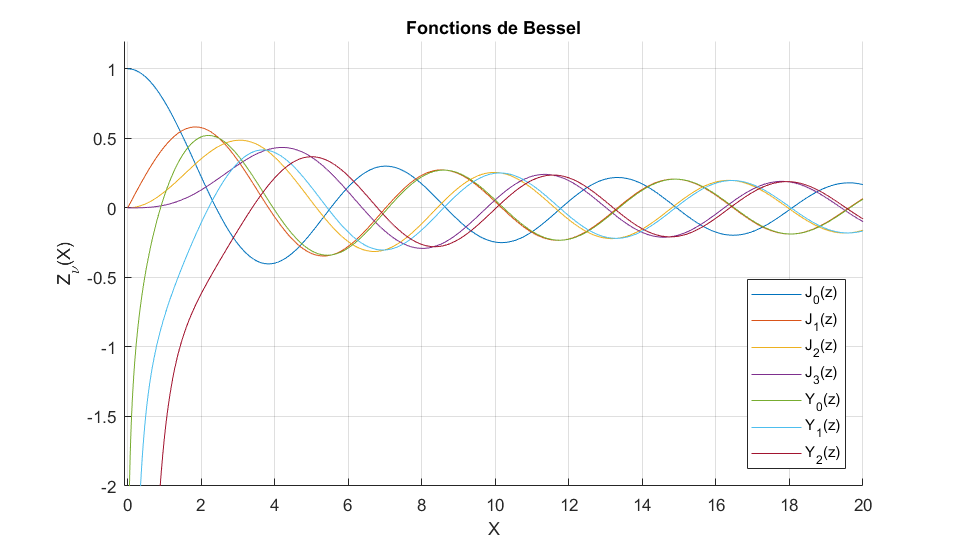
\includegraphics[width=\textwidth]{bessel_functions.png}
	\caption{Quelques fonctions de Bessel}
	\label{fig:wave_bessel_functions}
\end{figure}

En attendant de connaitre plus d'informations sur ces fonctions de Bessel, qui méritent toute une section, voyons déjà ce à quoi elles ressemblent. La figure~\ref{fig:wave_bessel_functions} présente les fonctions $J_0(z)$, $J_1(z)$ et $J_2(z)$, et $Y_0(z)$, $Y_1(z)$ et $Y_2(z)$. Les fonctions de Bessel du premier type sont toujours réguliers à l'origine pour des valeurs de $m$ entières positives ; $J_0(z)$ vaut $1$ à l'origine, tandis que les autres $J_m(z)$ y valent $0$. Les fonctions de Bessel du second type sont, à l'inverse, toujours singulières à l'origine : elles tendent vers $-\infty$ quand $z \Rightarrow 0^+$. On constate également que les fonctions de Bessel ressemblent à des (co)sinusoïdes amorties, avec des oscillations à intervalles réguliers et tendant vers $0$ quand $z \Rightarrow \infty$ (avec l'exception des fonctions $Y_m(z)$ qui divergent à l'origine).

Maintenant que l'on en sait un peu plus sur les fonctions de Bessel, poursuivons notre résolution du problème de Helmholtz. Les solutions de l'équation de Bessel, que respecte notre fonction $R_m(r)$ pour $m$ entier, étant les deux types de fonctions de Bessel d'ordre $m$, on peut donc écrire
\[ R_m(r) = C_m J_m(kr) + D_m Y_m(kr) \]
Il reste à appliquer les conditions limites. Nous avons une seule condition limite, $R_m(a) = 0$. Il nous en manque donc une ; de la même manière qu'avec l'équation de Laplace, nous souhaitons avoir une solution qui soit régulière (finie) en $r=0$ (vu qu'on a une membrane circulaire). Comme $Y_m(kr)$ est singulier en $r=0$, il faut donc s'en débarrasser en imposant $D_m = 0$, ce qui nous donne
\[ R_m(r) = C_m J_m(kr) \]

Maintenant, on applique notre condition limite,
\[ R_m(a) = C_m J_m(k a) = 0 \]
Comme on souhaite avoir une solution non triviale, il faut que $J_m(k a) = 0$, ce qui signifie qu'il nous faut les zéros des fonctions de Bessel. Malheureusement, ces zéros ne peuvent pas être calculés analytiquement, et il faut donc recourir à des méthodes numériques pour les trouver. Le n\ieme{} zéro de la fonction $J_m(z)$ est noté $j_{m, n}$
\footnote{En accord avec \href{http://mathworld.wolfram.com/BesselFunctionZeros.html}{Wolfram MathWorld} ; le cours utilise la notation $z_{m, n}$.} ;
le zéro d'indice $0$, $j_{m, 0}$, est généralement considéré comme l'origine (sauf pour $J_0(z)$, qui n'a pas de zéro $j_{0, 0}$). Les tables~\ref{tab:bessel_first_kind_zeros} et~\ref{tab:bessel_second_kind_zeros} donnent quelques-uns des zéros des fonctions de Bessel. A noter que pour $i \neq j$, les fonctions de Bessel $J_i(z)$ et $J_j(z)$ n'ont aucun zéro en commun, à l'exception de celui à l'origine (c'est l'\emph{hypothèse de Bourget}).

\begin{table}[t]
	\caption{Table des zéros des fonctions de Bessel du premier type}
	\label{tab:bessel_first_kind_zeros}
	\centering
	\begin{tabular}{ccccc}
	\toprule
	$k$ & $J_0(z)$ & $J_1(z)$ & $J_2(z)$ & $J_3(z)$ \\
	\midrule
	$1$ & $2.404826$ & $3.831706$ & $5.135622$ & $6.380162$ \\
	$2$ & $5.520078$ & $7.015587$ & $8.417244$ & $9.761023$ \\
	$3$ & $8.653728$ & $10.173468$ & $11.619841$ & $13.015201$ \\
	$4$ & $11.791534$ & $13.323692$ & $14.795952$ & $16.223466$ \\
	$5$ & $14.930918$ & $16.470630$ & $17.959819$ & $19.409415$ \\
	$\dots$ & $\dots$ & $\dots$ & $\dots$ & $\dots$ \\
	\bottomrule
	\end{tabular}
\end{table}

\begin{table}[t]
	\caption{Table des zéros des fonctions de Bessel du second type}
	\label{tab:bessel_second_kind_zeros}
	\centering
	\begin{tabular}{ccccc}
		\toprule
		$k$ & $Y_0(z)$ & $Y_1(z)$ & $Y_2(z)$ & $Y_3(z)$ \\
		\midrule
		$1$ & $3.957678$ & $2.197141$ & $3.384242$ & $4.527025$ \\
		$2$ & $7.086051$ & $5.429681$ & $6.793898$ & $8.097554$ \\
		$3$ & $10.222345$ & $8.596006$ & $10.023478$ & $11.396467$ \\
		$4$ & $13.361097$ & $11.749155$ & $13.209987$ & $14.623078$ \\
		$5$ & $16.500922$ & $14.897442$ & $16.378967$ & $17.818455$ \\
		$\dots$ & $\dots$ & $\dots$ & $\dots$ & $\dots$ \\
		\bottomrule
	\end{tabular}
\end{table}

\begin{table}[t]
	\caption{Table des zéros des dérivées des fonctions de Bessel du second type}
	\label{tab:bessel_derivative_first_kind_zeros}
	\centering
	\begin{tabular}{ccccc}
		\toprule
		$k$ & $J'_0(z)$ & $J'_1(z)$ & $J'_2(z)$ & $J'_3(z)$ \\
		\midrule
		$1$ & $0$ & $1.841184$ & $3.054237$ & $4.201189$ \\
		$2$ & $3.831706$ & $5.331443$ & $6.706133$ & $8.015237$ \\
		$3$ & $7.015587$ & $8.536316$ & $9.969468$ & $11.345924$ \\
		$4$ & $10.173468$ & $11.706005$ & $13.170371$ & $14.585848$ \\
		$5$ & $13.323620$ & $14.863589$ & $16.347522$ & $17.788748$ \\
		$\dots$ & $\dots$ & $\dots$ & $\dots$ & $\dots$ \\
		\bottomrule
	\end{tabular}
\end{table}

Bref, en notant $j_{m, n}$ le n\ieme{} zéro de la fonction de Bessel d'ordre $m$ $J_m(z)$, on doit donc avoir que $k\cdot a$ doit être l'un de ces zéros ; on peut donc écrire
\[ k a = j_{m, n} \]
soit, en supposant que $a \neq 0$, et en souhaitant $k \neq 0$
\begin{equation}
k_{m, n} = \frac{j_{m, n}}{a} \quad n=1, 2, \dots
\label{eq:wave_circular_kmn}
\end{equation}
et la constante $k$ dépend donc de nouveau de deux paramètres, $m = 0, 1, \dots$ qui décrit le nombre de périodes qu'accomplit $\Theta_m(\theta)$ lorsque $\theta$ varie de $0$ à $2\pi$ sur tout le cercle, et $n = 1, 2, \dots$, l'indice du n\ieme{} zéro de la fonction de Bessel $J_m(z)$, qui dépend elle-même du paramètre $m$.

La solution pour $R_{m, n}$ est donc
\[ R_{m, n} = C_{m, n} J_m(k_{m, n} r) = C_{m, n} J_m(z_{m, n} \frac{r}{a}) \]
et la solution pour $\phi = \phi_{m, n}(r, \theta)$ est donc
\begin{equation}
\begin{split}
\phi_{m, n} (r, \theta) = {} & C_{m, n} J_m(k_{m, n} r) \left( A_m \cos(m\theta) + B_m \sin(m \theta) \right) \\
= {} & A_{m, n}^* \cos(m\theta) J_{m}\left( j_{m, n} \frac{r}{a} \right) \\*
&+ B_{m, n}^* \sin(m\theta) J_{m}\left( j_{m, n} \frac{r}{a} \right)
\end{split}
\label{eq:wave_circular_phi_mn}
\end{equation}
avec $A_{m, n}^*=A_{m}C_{m, n}$ et $B_{m, n}^*=B_{m}C_{m, n}$. Les deux fonctions qui apparaissent (sans les constantes $A$ et $B$) sont dénommées \emph{modes propres de vibration d'une membrane circulaire}. Elles ont la propriété d'être orthogonales entre elles (problème de Helmholtz oblige).

Notre constante $k_{m, n}$ étant déterminée, on peut maintenant enfin résoudre la deuxième équation de notre première séparation de variables, celle du temps :
\[ \frac{1}{c^2} \frac{T''(t)}{T(t)} = -k_{m, n}^2 \]
dont la solution générale est bien entendu
\[ T_{m, n}(t) = C_{m, n}^* \cos(k_{m, n} c t) + D_{m, n}^* \sin(k_{m, n} c t) \]

Enfin, la solution générale de notre problème de vibration, sur un disque de rayon $a$, est
\begin{align}
u(r, \theta, t) &= \sum_{m=0}^{\infty} \sum_{n=1}^{\infty} u_{m,n} (r, \theta, t) \nonumber \\
&= \sum_{m=0}^{\infty} \sum_{n=1}^{\infty} \left( T_{m, n}(t) R_{m, n} (r) \Theta_m(\theta) \right) \\
&= \sum_{m=0}^{\infty} \sum_{n=1}^{\infty}
	\left( C_{m, n}^* \cos(k_{m, n} c t) + D_{m, n}^* \sin(k_{m, n} c t) \right)
	J_{m}\left( j_{m, n} \frac{r}{a} \right)
	\left( A_{m, n}^* \cos(m\theta) + B_{m, n}^* \sin(m \theta) \right) \label{eq:wave_circular_gensolution}
\end{align}

Et nous avons donc quatre familles de constantes à déterminer : $A_{m, n}^*$, $B_{m, n}^*$, $C_{m, n}^*$ et $D_{m, n}^*$, à partir de nos conditions initiales $u_0(r, \theta, 0)$ et $\dot{u}_0(r, \theta, 0)$.

Une remarque qui en vaut la peine : pour $m = 0$, nous trouvons le mode zéro en $\theta$, à qui correspond la fonction de Bessel $J_0(k_{0, n})$. On constate assez facilement que dans ce cas, le terme $\tilde{B}_{0, n} \sin(0 \cdot \theta)$ s'annule à cause du sinus, et donc le coefficient $\tilde{B}_{0, n}$ n'a aucune importance dans la solution, et on peut donc l'annuler. Quant à l'autre terme de la partie angulaire, il se simplifie en $\tilde{A}_{0, n}$, donnant une solution ne dépendant pas de l'angle $\theta$. Du coup, la solution peut en fait s'écrire de manière équivalente en
\begin{equation*}
\begin{split}
u(r, \theta, t) &= \sum_{n=1}^{\infty} \left( (A_{0, n}^* C_{0, n}^*) \cos(k_{0, n} c t) + (A_{0, n}^* D_{0, n}^*) \sin(k_{0, n} c t) \right)
	J_{0}\left( j_{0, n} \frac{r}{a} \right) \\
	&+ \sum_{m=1}^{\infty} \sum_{n=1}^{\infty}
	\left( C_{m, n}^* \cos(k_{m, n} c t) + D_{m, n}^* \sin(k_{m, n} c t) \right)
	J_{m}\left( j_{m, n} \frac{r}{a} \right)
	\left( A_{m, n}^* \cos(m\theta) + B_{m, n}^* \sin(m \theta) \right)
\end{split}
\end{equation*}

Exprimons les conditions :
\begin{align*}
u_0(r, \theta) = u(r, \theta, 0) = {} & \sum_{m=0}^{\infty} \sum_{n=1}^{\infty} C_{m, n}^* J_{m} \left( j_{m, n} \frac{r}{a} \right)
	\left( A_{m, n}^* \cos(m\theta) + B_{m, n}^* \sin(m \theta) \right)
\end{align*}
et
\begin{align*}
\dot{u}_0(r, \theta) &= \fpart{u}{t}(r, \theta, 0) \\
&= \sum_{m=0}^{\infty} \sum_{n=1}^{\infty} \Big( - C_{m, n}^* k_{m, n} c \sin(k_{m, n} c\cdot 0) + D_{m, n}^* k_{m, n} c \cos(k_{m, n} c\cdot 0) \Big) \\*
&\quad \cdot J_{m}\left( \frac{j_{m, n} r}{a} \right) \left( A_{m, n}^* \cos(m\theta) + B_{m, n}^* \sin(m \theta) \right) \\ \displaybreak[2]
&= \sum_{m=0}^{\infty} \sum_{n=1}^{\infty} D_{m, n}^* k_{m, n} c J_{m}\left( j_{m, n} \frac{r}{a} \right)
	\left( A_{m, n}^* \cos(m\theta) + B_{m, n}^* \sin(m \theta) \right)
\end{align*}
En supposant que $\dot{u}_0(r, \theta) = 0$ (vitesse initiale de la membrane nulle), nous devons avoir $D_{m, n}^* = 0$ pour avoir une solution non nulle. Si on avait $U_0(r, \theta) = 0$ à la place, c'était $C_{m, n}^* = 0$.

Avec une constante de moins\footnote{On aurait pu garder cette constante et faire le développement en toute généralité ; ça prend juste beaucoup de temps},
on peut à présent écrire notre solution sous la forme
\begin{align}
u(r, \theta, t) &= \sum_{m=0}^{\infty} \sum_{n=1}^{\infty} C_{m, n}^* \cos(k_{m, n} c t)
	J_{m}\left( j_{m, n} \frac{r}{a} \right)
	\left( A_{m, n}^* \cos(m\theta) + B_{m, n}^* \sin(m \theta) \right) \label{eq:wave_circular_nullspeed_pre_solution} \\
&= \sum_{m=0}^{\infty} \sum_{n=1}^{\infty} \cos(k_{m, n} c t) J_{m}\left( j_{m, n} \frac{r}{a} \right)
	\left( \tilde{A}_{m, n} \cos(m\theta) + \tilde{B}_{m, n} \sin(m \theta) \right) \label{eq:wave_circular_nullspeed_solution}
\end{align}
et notre condition initiale devient (ou plutôt, reste)
\begin{align}
u_0(r, \theta) = u(r, \theta, 0) &= \sum_{n=1}^{\infty}
	\underbrace{A_{0, n}^* C_{0, n}^*}_{=\tilde{A}_{0, n}}
	J_{0}\left( j_{0, n} \frac{r}{a} \right) + \sum_{m=1}^{\infty} \sum_{n=1}^{\infty} J_{m}\left( j_{m, n} \frac{r}{a} \right)
	\left( \tilde{A}_{m, n} \cos(m\theta) + \tilde{B}_{m, n} \sin(m \theta) \right) \label{eq:wave_circular_nullspeed_initial}
\end{align}

Cette simplification faite, comment peut-on déterminer les coefficients $\tilde{A}_{0, n}$, $\tilde{A}_{m, n}$ et $\tilde{B}_{m, n}$ ? Il va falloir faire preuve d'imagination ou plutôt, d'astuce. L'idée va être d'utiliser les propriétés d'orthogonalité des fonctions propres afin d'éliminer une partie des coefficients, et en même temps d'éliminer les coefficients qui ne nous intéressent pas.

Nous savons que\footnote{Rappelons que $\dif{S} = r \dif{r} \dif{\theta}$ et $\delta_{np}=0$ si $n\neq p$, $1$ sinon.}
\begin{gather}
\int \phi_1(r, \theta) \phi_2(r, \theta) = \int_{0}^{a} \dif{r} \int_{0}^{2\pi} \dif{\theta} \; r \phi_1(r, \theta) \phi_2(r, \theta) = 0 \label{eq:wave_circular_ortho_proper_functions} \\
\shortintertext{par orthogonalité des fonctions propres,}
\int_{0}^{2\pi} \sin (m\theta) \sin(n\theta) \dif{\theta} = \pi \delta_{mn} \label{eq:wave_circular_orthogonal_sinus} \\
\int_{0}^{2\pi} \cos(m\theta) \cos(n\theta) \dif{\theta} = \pi \delta_{mn} \label{eq:wave_circular_orthogonal_cos} \\
\int_{0}^{2\pi} \sin(m\theta) \cos(n\theta) \dif{\theta} = 0 \label{eq:wave_circular_orthogonal_sincos} \\
\shortintertext{et}
\int_{0}^{a} J_m\left(\frac{j_{m, n} r}{a}\right) J_m\left(\frac{j_{m, p} r}{a}\right) r \dif{r} = \frac{a^2}{2} J_{m+1} (j_{m, n})^2 \delta_{np} \label{eq:wave_circular_orthogonal_bessel}
\end{gather}
par orthogonalité des fonctions de Bessel. Cette dernière relation sera démontrée dans la section suivante.

Commençons par calculer les $\tilde{A}_{0, p}$. Pour cela, on multiplie~\eqref{eq:wave_circular_nullspeed_initial} par $r J_0(k_{0, p}r)$, et on intègre sur tout le cercle :
\begin{align*}
u_0(r, \theta) r J_0\left(\frac{j_{0, p} r}{a}\right) &= \sum_{n=1}^{\infty} \tilde{A}_{0, n} r J_0\left(\frac{j_{0, n} r}{a}\right) J_0\left(\frac{j_{0, p} r}{a}\right) \\*
	&\quad + \sum_{m=1}^{\infty} \sum_{n=1}^{\infty} r J_m\left(\frac{j_{m, n} r}{a}\right) J_0\left(\frac{j_{0, p} r}{a}\right) \left(\tilde{A}_{m, n}\cos m \theta + \tilde{B}_{m, n} \sin m \theta\right)
\end{align*}
\begin{align*}
I_{0, p} &= \int_{0}^{2\pi} \dif{\theta} \int_{0}^{a} \dif{r} \; u_0(r, \theta) r J_0\left(\frac{j_{0, p} r}{a}\right) \\ \displaybreak[2]
&= \sum_{n=1}^{\infty} \tilde{A}_{0, n} \underbrace{\int_{0}^{2\pi} \dif{\theta}}_{=2\pi}
	\int_{0}^{a} \dif{r} \; r J_0\left(\frac{j_{0, n} r}{a}\right) J_0\left(\frac{j_{0, p} r}{a}\right) \\ \displaybreak[1]
	&\quad + \sum_{m=1}^{\infty} \sum_{n=1}^{\infty} \Bigg(
	\underbrace{\int_{0}^{2\pi} \left(\tilde{A}_{m, n}\cos m \theta + \tilde{B}_{m, n} \sin m \theta\right)\dif{\theta} }_{ = 0 \text{ car tour complet des (co)sinus}} \cdot \int_{0}^{a} r J_m\left(\frac{j_{m, n} r}{a}\right) J_0\left(\frac{j_{0, p} r}{a}\right) \dif{r} \Bigg) \\ \displaybreak[2]
&= \sum_{n=1}^{\infty} \tilde{A}_{0, n} 2\pi \underbrace{\int_{0}^{a} r J_0\left(\frac{j_{0, n} r}{a}\right) J_0\left(\frac{j_{0, p} r}{a}\right) \dif{r}}_{= 0 \text{ si } p\neq n} \\
&= \tilde{A}_{0, p} 2\pi \int_{0}^{a} r J_0\left(\frac{j_{0, p} r}{a}\right)^2 \dif{r} \\
&= \tilde{A}_{0, p} \pi a^2 J_1(j_{0, p})^2
\end{align*}
soit
\begin{equation}
\tilde{A}_{0, p} = \frac{1}{\pi a^2 J_1(j_{0, p})^2} \int_{0}^{2\pi} \dif{\theta} \int_{0}^{a} \dif{r} \; u_0(r, \theta) r J_0\left(\frac{j_{0, p} r}{a}\right)
\label{eq:wave_circular_nullspeed_Atilde0p}
\end{equation}

Pour déterminer les $\tilde{A}_{p, q}$, $p, q > 0$, on multiplie cette fois par $J_p(k_{p, q}) \cos p\theta$, et on intègre :
\begin{align*}
u_0(r, \theta) r J_p\left(\frac{j_{p, q} r}{a}\right) \cos p \theta &=
	\sum_{n=1}^{\infty} \tilde{A}_{0, n} r J_0\left(\frac{j_{0, n} r}{a}\right) J_p\left(\frac{j_{p, q} r}{a}\right) \cos p \theta \\*
	&\quad + \sum_{m=1}^{\infty} \sum_{n=1}^{\infty} r J_m\left(\frac{j_{m, n} r}{a}\right) J_p\left(\frac{j_{p, q} r}{a}\right) \cos p \theta \left( \tilde{A}_{m, n}\cos m \theta + \tilde{B}_{m, n} \sin m \theta \right)
\end{align*}
\begin{align*}
I_{p, q} &= \int_{0}^{2\pi} \dif{\theta} \int_{0}^{a} \dif{r} \; u_0(r, \theta) r J_p\left(\frac{j_{p, q} r}{a}\right) \cos p\theta \\
&= \sum_{n=1}^{\infty} \tilde{A}_{0, n} \underbrace{\int_{0}^{2\pi} \cos p\theta \dif{\theta}}_{=0 \text{ car tour complet}}
	\int_{0}^{a} r J_0\left(\frac{j_{0, n} r}{a}\right) J_p\left(\frac{j_{p, q} r}{a}\right) \dif{r} \\ \displaybreak[1]
	&\quad + \sum_{m=1}^{\infty} \sum_{n=1}^{\infty} \Bigg(
	\int_{0}^{2\pi} \left(\tilde{A}_{m, n}\cos m \theta \cos p\theta + \tilde{B}_{m, n} \sin m \theta \cos p\theta \right)\dif{\theta} \cdot \int_{0}^{a} r J_m\left(\frac{j_{m, n} r}{a}\right) J_p\left(\frac{j_{p, q} r}{a}\right) \dif{r} \Bigg) \\ \displaybreak[2]
&= \sum_{m=1}^{\infty} \sum_{n=1}^{\infty} \Bigg(
	\underbrace{\int_{0}^{2\pi} \tilde{A}_{m, n} \cos m\theta \cos p\theta \dif{\theta}}_{=0 \text{ si } m\neq p}
	+ \underbrace{\int_{0}^{2\pi} \tilde{B}_{m, n} \sin m\theta \cos p\theta \dif{\theta}}_{=0} \Bigg) \cdot \qquad // \\%*
	% &\quad \cdot \int_{0}^{a} J_m\left(\frac{j_{m, n} r}{a}\right) J_p\left(\frac{j_{p, q} r}{a}\right) r \dif{r} \\
	\displaybreak[2]
&= \sum_{n=1}^{\infty} A_{p, n} \pi
	\underbrace{\int_{0}^{a} J_p\left(\frac{j_{p, n}r}{a}\right) J_p\left(\frac{j_{p, q}r}{a}\right) r \dif{r}}_{=0 \text{ si } n \neq q} \\
&= A_{p, q} \pi \int_{0}^{a} J_p\left(\frac{j_{p, q}r}{a}\right)^2 r \dif{r} \\
&= A_{p, q} \pi \frac{a^2}{2} J_{p+1}(j_{p, q})^2
\end{align*}
soit
\begin{equation}
\tilde{A}_{p, q} = \frac{1}{\pi \frac{a^2}{2} J_{p+1}(j_{p, q})^2} \int_{0}^{2\pi} \dif{\theta} \int_{0}^{a} \dif{r} \; u_0(r, \theta) r J_p\left(\frac{j_{p, q}r}{a}\right) \cos p\theta
\label{eq:wave_circular_nullspeed_Atildepq}
\end{equation}

Pour déterminer $\tilde{B}_{p, q}$, on multiplie cette fois par $J_p(k_{p, q}r) \sin p\theta$, et après un raisonnement similaire, on obtient
\begin{equation}
\tilde{B}_{p, q} = \frac{1}{\pi \frac{a^2}{2} J_{p+1}(j_{p, q})^2} \int_{0}^{2\pi} \dif{\theta} \dif{r} \int_{0}^{a} u_0(r, \theta) r J_p\left(\frac{j_{p, q}r}{a}\right) \sin p\theta
\label{eq:wave_circular_nullspeed_Btildepq}
\end{equation}

Comme on le voit, les expressions définissant les coefficients ne sont pas très gentils : ils requièrent de calculer l'intégrale du produit entre une fonction sur laquelle nous avons le contrôle (ou pas), $u_0(r, \theta)$, et une fonction de Bessel. En général, ces intégrales sont impossibles à calculer analytiquement. Mais il existe des cas particuliers, notamment les intégrales suivantes
\begin{gather*}
\int x^m J_0(x) \dif{x} = x^m J_1(x) + (m-1) x^{m-1} J_0(x) - (m-1)^2 \int x^{m-2} J_0(x) \dif{x} \\
\int x J_0(x) \dif{x} = x J_1(x) \\
\int x^2 J_0(x) \dif{x} = x^2 J_1(x) + x J_0(x) - \int J_0(x) \dif{x} \\
\int x^3 J_0(x) \dif{x} = x^3 J_1(x) + 2 x^2 J_0(x) - 4 x J_1(x)
\end{gather*}

Ces intégrales sont particulièrement utile dans le cas particulier où $u_0(r, \theta)$ ne dépend pas de $\theta$ (problème axisymétrique). A titre d'exemple, supposons que $u_0(r, \theta) = f(r)$, et voyons ce qu'il devient de nos intégrales :
\begin{align*}
\tilde{A}_{p, q} &= \frac{1}{\pi \frac{a^2}{2} J_{p+1}(j_{p, q})^2} \underbrace{\int_{0}^{2\pi} \cos p\theta \dif{\theta}}_{=0} \int_{0}^{a} f(r) r J_p\left(\frac{j_{p, q}r}{a}\right) \dif{r} \\
&= 0
\end{align*}
et pareillement pour $\tilde{B}_{p, q}$. Quand à $\tilde{A}_{0, p}$ :
\begin{align*}
\tilde{A}_{0, p} &= \frac{1}{\pi a^2 J_1(j_{0, p})^2} \int_{0}^{2\pi} \dif{\theta} \int_{0}^{a} f(r) r J_0\left(\frac{j_{0, p} r}{a}\right) \dif{r} \\
&= \frac{\int_{0}^{a} f(r) J_0\left(\frac{j_{0, p}r}{a}\right) \dif{r}}{\frac{a^2}{2} J_1(j_{0, p})^2}
\end{align*}
soit une expression un peu plus gentille. L'APE 7 utilise cette expression pour trouver les coefficients, vu que la fonction est connue.

\subsection{Conclusion et complications possibles}

Nous avons donc pu résoudre l'équation d'onde, sur une membrane circulaire fixée sur son bord, avec une vitesse initiale nulle, et avec une symétrie axiale au niveau de la condition initiale, et donc une solution avec une symétrie axiale. Il s'agit de beaucoup de conditions supplémentaires ; voyons ce qu'il se passe quand on enlève une à une les conditions.

\subsubsection{Condition initiale non axisymétrique}

Dans ce cas, les coefficients $\tilde{A}_{p, q}$ et $\tilde{B}_{p, q}$ ne seront pas forcément nuls.

La condition axisymétrique imposait une symétrie axiale de la solution, similaire à la symétrie axiale de la situation initiale. Cela imposait que les termes de la solution~\ref{eq:wave_circular_nullspeed_solution} qui dépendaient de $\theta$ s'en aille, et c'est exactement ce qu'il s'est passé pour les $\tilde{A}_{p, q}$ et $\tilde{B}_{p, q}$ pour $p>0$ : ils se sont annulés.

Dans le cas un peu plus générale d'une condition initiale non symétrique, il faudra calculer ces coefficients, avec du coup une double intégrale compliquée. Si $u_0(r, \theta) = f(r)g(\theta)$, et que $f(r)$ est une fonction sympathique, il est possible de séparer la double intégrale en deux intégrales, et de calculer ces deux intégrales, de manière classique pour $\theta$, de manière plus douloureuse pour $r$ (à cause des fonctions de Bessel). Malheureusement, il y a peu de fonctions gentilles lorsqu'on les intègre avec les fonctions de Bessel d'ordre supérieur à 0\dots

\subsubsection{Vitesse initiale non nulle}

Si la vitesse initiale n'est pas nulle, le coefficient $D^*_{m, n}$ ne sera pas non plus nul, et il y aura donc un total de 4 coefficients à calculer : $A^*_{m, n}C^*_{m, n}=\tilde{A}_{m, n}$, $B^*_{m, n}C^*_{m, n}=\tilde{B}_{m, n}$, $A^*_{m, n}D^*_{m, n}=\tilde{C}_{m, n}$ et $B^*_{m, n}D^*_{m, n}=\tilde{D}_{m, n}$. Heureusement, de la même manière que la condition initiale $u_0$ n'a besoin que des coefficients $\tilde{A}_{m, n}$ et $\tilde{B}_{m, n}$, la condition de vitesse initiale n'aura besoin que de $\tilde{C}_{m, n}$ et $\tilde{D}_{m, n}$ : il n'y a, pour chaque condition initiale, que deux familles de constantes à calculer\footnote{Ainsi que le mode zéro, $\tilde{A}_{0, n}$ ou $\tilde{C}_{0, n}$, qui engendre quelques petites simplifications à prendre en compte, et qui justifie de le séparer lors du calcul.}
et donc, il y a largement moyen d'appliquer les mêmes méthodes que ci-dessus pour obtenir les coefficients.

\subsubsection{Condition limite de Neumann ou de Robin}

Lors de notre résolution, nous avons considéré que la membrane était fixé sur les bords, et donc qu'il y avait des conditions limites homogènes de Dirichlet sur les bords du domaine. Cela nous a permis d'exprimer la condition sur $R(a)$, qui a débouché sur la nécessité que $k_{m, n}=\frac{j_{m, n}}{a}$, et d'utiliser les zéros de $J_m$.

Il est possible de généraliser ce procédé pour des conditions limites homogènes de Neumann $\dot{u}(a, \theta, t) = 0$ et de Robin $\dot{u}(a, \theta, t) = \mathcal{C}\cdot u(a, \theta, t)$. Dans le premier cas, il faudra utiliser des zéros des dérivées des fonctions de Bessel, et dans le second cas, quelque chose de plus compliqué. %TODO

L'orthogonalité des fonctions de Bessel est toujours assuré pour ces zéros (démontré dans la section suivante), et on peut donc sereinement résoudre notre problème.

\subsubsection{Domaine en forme d'anneau}

Si notre domaine n'était pas un cercle mais un anneau, nous n'aurions pas pu éliminer $Y_m(z)$ de la solution car $r=0$ ne fait pas partie du domaine, et il aurait donc fallu tenir compte des deux fonctions de Bessel. Dans le cas de conditions aux limites de Dirichlet, il faut donc satisfaire une équation plus compliquée, qui malheureusement requiert des méthodes numériques. % TODO flemme de chercher, mais ça peut être utile de voir ce qu'il se passe sur un anneau

\section{Les fonctions de Bessel}

Dans cette section, les fonctions de Bessel jouent un rôle primordial. Il est donc intéressant d'en connaitre un peu plus sur ces fameuses fonctions.

Comme indiqué lors de leur présentation, ces fonctions ne peuvent pas être exprimées à partir des fonctions classiques (fonctions trigonométriques, hyperboliques, logarithmes, exponentielles\dots). Leur seule vraie définition est qu'elles respectent l'équation de Bessel, que les deux types de solutions sont linéairement indépendantes, et que le premier type n'a pas de singularité à l'origine pour des valeurs de $m$ entières ou positives, et diverge en $0$ pour des valeurs de $m$ négatives et non entières, tandis que le deuxième type est toujours singulier à l'origine et multiforme. Il existe néanmoins des expressions analytiques non finies pour ces fonctions. Par exemple, l'expansion de $J_m(z)$ en série de Taylor autour de $z=0$ est
\begin{equation}
J_m(z) = \sum_{n=0}^{\infty} \frac{(-1)^n}{n! \Gamma(n+m+1)} \left( \frac{x}{2} \right)^{2n + m}
\label{eq:wave_bessel_first_kind_series}
\end{equation}
où $\Gamma(x)$ désigne la fonction $\Gamma$, généralisation de la factorielle sur les complexes\footnote{La fonction n'a un comportement de factorielle que sur les réels positifs ; ailleurs ça devient n'importe quoi.}.

Le lecteur intéressé se demande peut-être comment cette expression a été trouvée. Même si ce n'est pas nécessaire pour comprendre le cours, la méthode de résolution de ce type d'équation, la méthode de Frobenius, nous apprend beaucoup de chose. Cette méthode permet de résoudre les équations de la forme
\[ z^2 u'' + p(z) u' + q(z) u = 0 \]
lorsque les fonctions $\frac{p(z)}{z}$ ou $\frac{q(z)}{z^2}$ ne sont pas analytiques (finies) en $z=0$ (ce qui empêche de résoudre l'équation en déterminant la série de Taylor), mais que $p(z)$ et $q(z)$ sont analytiques en $z=0$\footnote{En fait, il suffit que $p(z)$ et $q(z)$ soient analytiques partout ailleurs que $0$, et que leur limite en $z=0$ existe et est finie.}.

Pour cela, on suppose que notre solution a la forme
\begin{equation}
u(z) = \sum_{k=0}^{\infty} A_k z^{k + r}
\label{eq:wave_bessel_frobenius_solpattern}
\end{equation}
où $r$ est un nombre, pas forcément entier, que nous allons devoir déterminer, et qui va nous permettre de calculer notre série (qui n'est pas de Taylor, car les exposants peuvent ne pas être entiers).

Injectons donc dans notre équation de Bessel, pour un $m$ fixé (pas forcément entier) :
\begin{align*}
0 &= z^2 u''(z) + z u'(z) + (z^2 - m^2) u(z) \\
&= z^2 \left( \sum_{k=0}^{\infty} A_k z^{k + r} \right)'' + z \left( \sum_{k=0}^{\infty} A_k z^{k + r} \right)' + (z^2 - m^2) \sum_{k=0}^{\infty} A_k z^{k + r} \\
&= z^2 \left( \sum_{k=0}^{\infty} (k+r)(k+r-1) A_k z^{k + r - 2} \right) + z \left( \sum_{k=0}^{\infty} (k+r) A_k z^{k + r - 1} \right) + (z^2 - m^2) \sum_{k=0}^{\infty} A_k z^{k + r} \\
&= \left( \sum_{k=0}^{\infty} (k+r)(k+r-1) A_k z^{k + r - 2} z^2 \right) + \left( \sum_{k=0}^{\infty} (k+r) A_k z^{k + r - 1} z \right) + (z^2 - m^2) \sum_{k=0}^{\infty} A_k z^{k + r} \\
&= \sum_{k=0}^{\infty} (k+r)(k+r-1) A_k z^{k + r} + (k+r) A_k z^{k + r} + A_k z^{k + r + 2} - m^2 A_k z^{k+r} \\
&= \sum_{k=0}^{\infty} z^{k+r} \left( (k+r)(k+r-1) A_k + (k+r) A_k - m^2 A_k \right) + \sum_{k'=0}^{\infty} A_{k'} z^{k' + r + 2} \\
&= \sum_{k=0}^{\infty} z^{k+r} \left((k+r)^2 - m^2\right) A_k + \sum_{k=2}^{\infty} A_{k-2} z^{k + r} \\
0 &= z^r (r^2-m^2)A_0 + z^{r+1} ((r+1)^2-m^2) A_1 \sum_{k=2}^{\infty} z^{k+r} \left( ((k+r)^2 - m^2) A_k + A_{k-2} \right)
\end{align*}
Pour que les deux membres soient nuls, il faut que chaque coefficient devant les puissances de $z$ soit nul. Il faut donc que
\begin{gather}
(r^2-m^2) A_0 = 0 \\
((r+1)^2-m^2) A_1 = 0 \\
((k+r)^2-m^2) A_k + A_{k-2} = 0 \quad \forall k>2 \label{eq:wave_bessel_frobenius_recurse}
\end{gather}
On s'impose $A_0 \neq 0$ pour garantir une seule représentation de l'équation, ce qui impose $r = \pm m$.

Dans le cas où $r=m$, on a alors que $((r+1)^2-m^2)A_1 = (2m+1)A_1=0$, ce qui donne $A_1=0$, sauf si $m=\frac{-1}{2}$. Dans ce dernier cas, la relation~\ref{eq:wave_bessel_frobenius_recurse} devient
\[ ((k-\frac{1}{2})^2-\frac{1}{4})A_k + A_{k-2} = (k^2-k)A_k + A_{k-2} = 0 \]
soit la relation de récurrence
\[ A_k = \frac{-A_{k-2}}{k(k-1)} \]
qui donne, après un bref développement, les relations suivantes
\begin{align*}
A_{2l} &= \frac{(-1)^l}{(2l)!} A_0 \\
A_{2l+1} &= \frac{(-1)^l}{(2l+1)!} A_1
\end{align*}
En réinjectant ces expressions dans l'équation~\ref{eq:wave_bessel_frobenius_solpattern}, on obtient
\begin{align*}
u(z) &= z^\frac{-1}{2} \sum_{k=0}^{\infty} A_k z^k \\
&= z^\frac{-1}{2} \left( \sum_{l=0}^{\infty} A_{2l} z^{2l} + \sum_{l=0}^{\infty} A_{2l+1} z^{2l+1} \right) \\
&= z^\frac{-1}{2} \left( A_0 \sum_{l=0}^{\infty} \frac{(-1)^l}{(2l)!} z^{2l} + A_1 \sum_{l=0}^{\infty} \frac{(-1)^l}{(2l+1)!} z^{2l+1} \right) \\
&= z^\frac{-1}{2} (A_0 \cos(z) + A_1 \sin(z))
\end{align*}
ce qui donne une double famille de solution. Il se fait que si l'on avait regardé la solution pour $r=-m$, nous aurions eu exactement le même soucis avec $m=\frac{1}{2}$, et nous aurions obtenu, au signe près, la même expression. Pour des raisons de normalisation et de continuité de certaines fonctions, on définit les fonctions de Bessel associées à $\pm\frac{1}{2}$ comme
\begin{align}
J_{-1/2}(z) &= \sqrt{\frac{2}{\pi z}} \cos(z) \\
J_{1/2}(z) &= \sqrt{\frac{2}{\pi z}} \sin(z)
\end{align}
et il s'agit des deux solutions indépendantes pour l'équation de Bessel avec $m=\pm\frac{1}{2}$.

Dans le cas où $m\neq \pm\frac{1}{2}$ (mais on considère encore que $r=m$), on a nécessairement $A_1=0$, et comme l'équation~\ref{eq:wave_bessel_frobenius_recurse} est toujours valide, on a
\begin{align*}
0&= (k^2 + 2km) A_k + A_{k-2} \\
A_k &= \frac{-1}{k(k+2m)} A_{k-2} \\
\Rightarrow A_{2l+1} &= 0 \\
\Rightarrow A_{2l} &= \frac{(-1)^l}{(2l)\cdot(2l-2)\cdot\dots\cdot(2) \cdot (2l+2m)\cdot(2l-2+2m)\cdot\dots\cdot(2+2m)\cdot(2m)} A_0 \\
&= \frac{(-1)^l}{2^l \cdot l\cdot(l-1)\cdot\dots\cdot1 \cdot 2^l \cdot (m+1)\cdot(m+2)\cdot\dots\cdot(m+l-1)\cdot(m+l)} A_0 \\
&= \frac{(-1)^l m!}{2^{2l} l! (m+l)!} A_0
\end{align*}
où $m!=m\cdot(m-1)\cdot\dots$, avec une limite encore incertaine (et non nécessaire car les coefficients se simplifie). On définit alors la fonction $\Gamma(m) = (m-1)!$, qui généralise la factorielle pour des nombres non entiers, et même complexes. On obtient alors
\begin{align*}
u(z) &= z^m \sum_{k=0}^{\infty} A_k z^{k} \\
&= \sum_{l=0}^{\infty} \frac{(-1)^l \Gamma(m+1)}{2^{2l} l! \Gamma(m+l+1)} A_0 z^{2l+m}
\end{align*}
ce qui, pour des raisons évidentes de clarté, est multiplié par $\frac{1}{\Gamma(m+1) 2^{m} A_0}$, qui ne sont de toutes façons que des constantes, pour donner la définition générale des fonctions de Bessel du premier type
\begin{equation}
J_m(z) = \sum_{l=0}^{\infty} \frac{(-1)^l}{l! \Gamma(m+l+1)} \left(\frac{z}{2}\right)^{2l+m}
\end{equation}

Et que dire du cas où $r=-m$ ? Dans ce cas, on a plutôt
\begin{align*}
0&= (k^2 - 2km) A_k + A_{k-2} \\
A_k &= \frac{-1}{k(k-2m)} A_{k-2} \\
\Rightarrow A_{2l+1} &= 0 \\
\Rightarrow A_{2l} &= \frac{(-1)^l}{(2l)\cdot(2l-2)\cdot\dots\cdot(2) \cdot (2l-2m)\cdot(2l-2-2m)\cdot\dots\cdot(2-2m)\cdot(-2m)} A_0 \\
&= \frac{(-1)^l}{2^l \cdot l\cdot(l-1)\cdot\dots\cdot1 \cdot 2^l \cdot (-m+1)\cdot(-m+2)\cdot\dots\cdot(-m+l-1)\cdot(-m+l)} A_0 \\
&= \frac{(-1)^l (-m)!}{2^{2l} l! (-m+l)!} A_0
\end{align*}
soit la même forme de solution (malgré l'étrangeté de la factorielle). C'est normal : le signe de $m$ n'intervient pas dans l'équation de Bessel. Les fonctions $J_m(z)$ et $J_{-m}(z)$ sont donc toutes les deux des solutions valides, et différentes (à cause de la fonction $\Gamma$). On peut montrer que si $m$ n'est pas un entier, ces deux fonctions sont effectivement linéairement indépendantes, et donc sont les deux solutions de l'équation de Bessel. % TODO rechercher pourquoi

Quand $m$ est entier par contre, les choses se gâtent : en effet, la fonction $\Gamma$ diverge vers l'infini aux entiers négatifs ou nuls. Pour $m\ge 0$, cela ne pose pas de problème, l'argument de $\Gamma$ reste supérieur à $0$. Mais pour $m < 0$, certains termes sont nuls. Pour $m>0$, calculons $J_{-m}(z)$ :
\begin{align*}
J_{-m}(z) &= \sum_{l=0}^{\infty} \frac{(-1)^l}{l! \Gamma(l+1-m)} \left(\frac{z}{2}\right)^{2l-m} \\
&= \sum_{l'=-m}^{\infty} \frac{(-1)^{l'+m}}{(l'+m)!\Gamma(l'+1)} \left(\frac{z}{2}\right)^{2l'+m} \\
&= \sum_{l'=-m}^{-1} \frac{(-1)^{l'+m}}{(l'+m)!\underbrace{\Gamma(l'+1)}_{=\infty}} \left(\frac{z}{2}\right)^{2l'+m} + \sum_{l'=0}^{\infty} \frac{(-1)^{l'+m}}{(l'+m)!\Gamma(l'+1)} \left(\frac{z}{2}\right)^{2l'+m} \\
&= (-1)^m \sum_{l'=0}^{\infty} \frac{(-1)^{l'}}{(l'+m)!l'!} \left(\frac{z}{2}\right)^{2l'+m} \\
&= (-1)^m J_m(z)
\end{align*}
et donc, les deux solutions potentielles ne sont pas linéairement indépendantes : il en manque une !

Pour la trouver, on définit une combinaison linéaire bizarre de $J_m(z)$, la fonction de Bessel du second type $Y_m(z)$ :
\begin{equation}
Y_m(z) = \frac{J_m(z)\cos(m z) - J_{-m}}{\sin(m z)}
\label{eq:wave_bessel_second_kind_from_first_nonint}
\end{equation}
Pour $m$ non entier, tout va bien, il s'agit bien d'une combinaison linéaire de deux fonctions linéairement indépendantes. Pour $m$ entier en revanche, il faut prendre la limite :
\begin{equation}
Y_m(z) = \lim\limits_{\alpha \to m} Y_\alpha(z) \quad m \in \mathbb{Z}, \alpha\not\in\mathbb{Z}
\label{eq:wave_bessel_second_kind_from_first_intm}
\end{equation}
ce qui permet de définir par des séries la valeur de $Y_m(z)$, mais difficilement : toutes les fonctions de Bessel du deuxième type divergent en $0$.

À partir de ces expressions et de l'équation de Bessel, on peut montrer que pour des valeurs entières de $m$ (ce qui nous intéresse généralement), la fonction de Bessel du premier type est une \emph{fonction entière}\footnote{La partie sur les fonctions complexes définit les fonctions holomorphiques et les fonctions entières ; pour le moment, une approximation est qu'il s'agit d'une fonction qui est égale à sa série de Fourier en tout point du plan complexe.},
et que pour des valeurs de $m$ non entières, elle est multiforme\footnote{De nouveau, on verra dans la partie complexe ce que ça signifie.}.

Pour des valeurs entières de $m$\footnote{On peut même généraliser à des valeurs non entières, via
\begin{equation}
J_m(z) = \frac{1}{\pi} \int_{0}^{\pi} \cos(m\tau - z\sin\tau) \dif{\tau} - \frac{\sin(m\pi)}{\pi} \int_{0}^{\infty} e^{-z\sinh(\tau) - m\tau} \dif{\tau}
\label{eq:wave_bessel_first_kind_overintegral}
\end{equation}},
on a aussi
\begin{equation}
J_m(z) = \frac{1}{\pi} \int_{0}^{\pi} \cos(m \tau - z\sin(\tau)) \dif{\tau} = \frac{1}{2\pi} \int_{-\pi}^{\pi} e^{i(m\tau - z\sin(\tau))} \dif{\tau}
\label{eq:wave_bessel_first_kind_integral}
\end{equation}

A la différence de $J_m(z)$, qui est régulier (fini) en $z=0$ pour des valeurs entières de $m$, $Y_m(z)$ a une singularité en $z=0$ (elle diverge) et est multiforme\footnote{Promis, dans la deuxième partie du syllabus, vous comprendrez tout !}. À la ressemblance de $Y_m(z)$, pour $m$ entier, on a $Y_{-m}(z)=(-1)^m Y_m(z)$. $J_m(z)$ et $Y_m(z)$ ont également la propriété d'être holomorphiques sur tout le plan complexe à l'exception des réels négatifs.

Tout ceci est intéressant, mais en pratique, à quoi ressemblent ces fonctions ? La figure~\ref{fig:wave_bessel_functions} montre un graphique des fonctions de Bessel $J_0(z)$, $J_1(z)$, $J_2(z)$, $Y_0(z)$, $Y_1(z)$ et $Y_2(z)$. On peut constater les propriétés suivantes :
\begin{itemize}
	\item Les fonctions de Bessel ressemblent à des sinusoïdales, avec des oscillations à intervalles réguliers, amorties par un facteur, qui s'avère être égal à $1/\sqrt{z}$ (on peut l'obtenir à partir de la série).
	\item La fonction de Bessel $J_0(z)$ vaut $1$ à l'origine, tandis que les autres fonctions de Bessel $J_m(z)$ pour $m>0$ entier valent $0$ à l'origine.
	\item Toutes les fonctions de Bessel $Y_m(z)$ tendent vers $-\infty$ lorsque $x\Rightarrow 0^+$, et sont donc singulières à l'origine.
\end{itemize}

Il est aussi possible de définir un comportement asymptotique à nos fonctions de Bessel :
\begin{itemize}
	\item Pour $m$ naturel non nul et pour $0 < z \ll \sqrt{m+1}$, on a
	\begin{align}
	J_m(z) &\approx \frac{z^m}{m!2^m}
	\label{eq:wave_bessel_first_kind_asymp0_intm} \\
	Y_m(z) &\approx \frac{-2^m (m-1)!}{\pi} z^{-m} \quad m\in \mathbb{C} \text{ aussi}
	\label{eq:wave_bessel_second_kind_asymp0_intm}
	\end{align}
	\item Pour $m=0$ et $0 < z < 1$, on a
	\begin{align}
	J_0(z) &\approx 1 \label{eq:wave_bessel_first_kind_asymp0_0} \\
	Y_0(z) &\approx \frac{2}{\pi}\left(\ln\left(\frac{z}{2}\right) - \gamma\right)
	\label{eq:wave_bessel_second_kind_asymp0_0gamma}
	\end{align}
	\item Pour $m$ naturel non nul et pour $z \gg 0$, on a
	\begin{align}
	J_m(z) &\approx \sqrt{\frac{2}{\pi z}} \cos\left( z-\frac{m\pi}{2} - \frac{\pi}{4} \right) \quad z\gg \abs{m^2-\frac{1}{4}}
	Y_m(z) &\approx \sqrt{\frac{2}{\pi z}} \sin\left( z-\frac{m\pi}{2} - \frac{\pi}{4} \right)
	\end{align}
\end{itemize}
Quel est ce $\gamma$ ? Il s'agit de la constante d'Euler-Mascheroni\footnote{Les deux premiers mathématiciens à avoir explicitement écrit des expressions utilisant cette constante sont Leonhard Euler et Lorenzo Mascheroni, et la première personne à avoir écrit cette constante sous le nom de $\gamma$ est Carl Anton Bretschneider. Parfois, les mathématiques pourraient être plus simples.}, qui est définie par
\[ \gamma = \lim\limits_{n\to\infty} \left( -\ln(n) +\sum_{k=0}^{n} \frac{1}{k} \right) = \int_{0}^{\infty} \frac{1}{\lfloor x \rfloor} - \frac{1}{x} \dif{x} \]
En pratique, on peut encore écrire
\begin{equation}
Y_0(z) \approx \frac{2}{\pi} \ln(z) \label{eq:wave_bessel_second_kind_asymp0_0nogamma}
\end{equation}

Une autre propriété sympathique des fonctions de Bessel sont les relations de récurrence
\begin{align}
\frac{2m}{z} Z_m(z) &= Z_{m-1}(z) + Z_{m+1}(z)
\label{eq:wave_bessel_recursive_normal} \\
2 \fdif{Z_m}{z}(z) &= Z_{m-1}(z) - Z_{m+1}(z)
\label{eq:wave_bessel_recursive_derivative}
\end{align}
où $Z_m$ désigne $Y_m$ ou $J_m$.

Ou encore, des relations d'intégration et de dérivation :
\begin{gather}
\fdif{}{z} (z^m J_m(z)) = z^m J_{m-1}(z) \\
\int_{0}^{a} z J_0(z) \dif{z} = z J_1(z)
\end{gather}

Notons enfin qu'il existe une \emph{équation modifiée de Bessel},
\[ z^2 R_m''(z) + z R_m'(z) - (z^2 + m^2) R(z) = 0 \]
dont les solutions sont les \emph{fonctions modifiées de Bessel},
\begin{align*}
I_m(z) &= i^{-m} J_m(i z) \\
K_m(z) &= \lim\limits_{\alpha \Rightarrow m} \frac{\pi}{2} \frac{I_{-\alpha}(z) - I_\alpha(z)}{\sin(\alpha z)}
\end{align*}
et qui ont la propriété de croitre et de décroitre de manière exponentielle ; c'est une des raisons pour lesquelles nous ne pouvions pas choisir une valeur négative pour $\lambda$.%En fait, I_m(0)=0 sauf I_0(0)=1, exponentiel, et K_m(0) se comporte comme -ln(z)

\subsection{Orthogonalité des fonctions de Bessel}

A la section précédente, nous avons utilisé, sans le prouver formellement, que les fonctions de Bessel d'ordre $m$ associées à des valeurs propres différentes sont orthogonales. Il est temps de combler ce manque.\footnote{Cette section s'inspire fortement de~\cite{lambers}}

Rappelons l'équation de Bessel, ou plutôt une de ses variantes,
\[ r^2\ffdif{J_m}{r}(kr) + r\fdif{J_m}{r}(kr) + (k^2r^2-m^2)J_m(kr) \]
$k^2$ étant sensé être une valeur propre, on réarrange les termes pour faire apparaitre la notation $A(x)=\lambda x$ :
\[ \left( -\ffdif{}{r} - \frac{1}{r} \fdif{}{r} + \frac{m^2}{r^2} \right)(J_m(kr)) = k^2 J_m(kr) \]
ce qui signifie que $k^2$ sera une valeur propre de l'opérateur
\[ \mathcal{L} = \left( -\ffdif{}{r} - \frac{1}{r} \fdif{}{r} + \frac{m^2}{r^2} \right) \]
avec comme fonction propre associée $J_m(kr)$.

Si notre problème de Helmholtz était bien auto-adjoint par rapport au produit scalaire habituel (l'intégrale du produit de deux fonctions), cet opérateur ne l'est pas ; en effet, $p_0(r) = -1$ et $p_1(r)=-\frac{1}{r}$. Néanmoins, on peut sauver la mise en utilisant un produit scalaire différent,
\[ \langle f_1, f_2 \rangle = \int_{0}^{a} w(r) f_1(r) F_2(r) \dif{r} \]
où $w(r)$ est une fonction de pondération de l'intégrale. Cette fonction se trouve en calculant
\[ \frac{1}{p_0(r)} e^{\int \frac{p_1(r)}{p_0(r)}\dif{r}} = -e^{\int \frac{1}{r} \dif{r}} = -e^{\ln(r) + k} = -e^k r \]
soit $w(r)=r$, pour simplifier les notations.

On calcule alors le produit scalaire de deux fonctions propres $J_m(kr)$ et $J_m(k'r)$, pour $k\neq k'$ :
\begin{align*}
\langle J_m(kr), J_m(k'r) \rangle &= \int_{0}^{a} w(r) J_m(kr) J_m(k'r) \dif{r} \\
&= \frac{1}{k^2 - k'^2} \left[ w(r) p_0(r) \Big(J_m(kr) J'_m(k'r) k' - J'_m(kr) k J_m(k'r)\Big) \right]_0^a \\
&= \frac{-a}{k^2 - k'^2} \Big(k' J_m(ka) J'_m(k'a) - k J'_m(ka) J_m(k'a)\Big)
\end{align*}
et donc, pour avoir l'orthogonalité, il faut que $k' J_m(ka) J'_m(k'a) = k J_m(k'a) J'_m(ka)$. Cela arrive dans les cas suivants :
\begin{itemize}
	\item $ka$ et $k'a$ sont des zéros de $J_m(z)$. C'est le cas que l'on utilise quand on résout le problème de Helmholtz sur une membrane circulaire fixée sur les bords, avec une condition de Dirichlet.
	\item $ka$ et $k'a$ sont des zéros de la dérivée, $J'_m(z)$. C'est le cas que l'on utiliserait si la membrane n'était pas fixée sur les bords, mais que l'on imposait une membrane horizontale au niveau des bords, avec des conditions de Neumann.
	\item $ka$ est un zéro de $J_m(z)$, et $k'a$ est un zéro de $J'_m(z)$ (ou inversement). Ce cas est rarement utilisé. % Vraiment ?
	\item On a juste $\frac{J_m(ka)}{k J'_m(ka)} = \frac{J_m(k'a)}{k' J'_m(k'a)} = C$. C'est le cas que l'on utiliserait si on avait une condition de Robin sur les bords, avec une relation de proportionnalité entre la pente de la fonction et sa hauteur sur le bord.
\end{itemize}

Dans ces 4 cas, on a bien orthogonalité des fonctions propres (fonctions de Bessel du même ordre mais reliées à des zéros différents), ce qui nous permet d'utiliser l'orthogonalité dans~\eqref{eq:wave_circular_orthogonal_bessel}.

% Wolfram est plus précis :
% int_0^a x J_n\left(\frac{j_{n, k}x}{a}\right)^2 \dif{x} =
% $\frac{a^2}{2} \left( J_n(j_{n, k})^2 - \frac{2 n J_{n+1}(j_{n, k}) J_n(j_{n, k})}{j_{n, k}} + J_{n+1}(j_{n, k})^2\right)$

Il est important de remarquer que la relation d'orthogonalité obtenue ici est légèrement différente des relations habituelles d'orthogonalité : ici, l'intégrale utilisée pour le produit scalaire requiert une fonction de pondération. En pratique, comme l'équation de Bessel apparait plutôt dans des problèmes à géométrie circulaire, et que la fonction de pondération est exactement le jacobien du changement de variable de rectangulaire à polaire\footnote{Voir annexe. TODO},%TODO
on utilise toujours cette expression du produit scalaire quand on doit utiliser l'orthogonalité des fonctions de Bessel.

Maintenant que l'on a démontré que les fonctions de Bessel $J_m(kr)$ et $J'_m(k'r)$, avec des $k$ et $k'$ associés à des zéros différents, déterminons la valeur du produit scalaire d'une fonction de Bessel avec elle-même.
\begin{align*}
\langle J_m(kr), J_m(kr) \rangle &= \int_{0}^{a} J_m(kr)^2 r \dif{r} \\
&= \lim\limits_{k' \to k} \frac{a\left(k' J_m(ka) J'_m(k'a) - k J_m(k'a) J'_m(ka) \right)}{k^2-k'^2} \\
\shortintertext{Le numérateur et le dénominateur s'annulent ; utilisons la règle de l'Hospital-Bernoulli :}
&= \lim\limits_{k' \to k} \frac{a\left(k' J_m(ka) J'_m(k'a) - k J_m(k'a) J'_m(ka) \right)'}{-2k'} \\
\shortintertext{En faisant l'hypothèse que $J_m(ka)=0$ (ce qui est le cas dans nos exemples),}
&= \lim\limits_{k' \to k} \frac{- a k (J_m(k'a) J'_m(ka))'}{-2k'} \\
&= \lim\limits_{k' \to k} \frac{- a k J'_m(k'a) a J'_m(ka)}{-2k'} \\
&= \frac{a^2 (J'_m(ka))^2}{2} = \frac{a^2}{2} (J'_m(ka))^2 \addtocounter{equation}{1} \tag{\theequation} \label{eq:wave_bessel_orthogonal_norm_1}
\end{align*}
ce que l'on peut encore simplifier en utilisant l'équation~\ref{eq:wave_bessel_recursive_derivative} :
\begin{align}
\int_{0}^{a} J_m(kr)^2 r \dif{r} &= \frac{a^2}{2} (J'_m(ka))^2 \nonumber \\
&= \frac{a^2}{2} \left( \frac{m}{z}J_m(ka) - J_{m+1} (ka) \right) \nonumber \\
&= \frac{a^2}{2} (J_{m+1}(ka))^2 \label{eq:wave_bessel_orthogonal_norm_2}
\end{align}

% TODO fonctions de Bessel sphériques ?
% TODO on retrouve les fonctions de Bessel avec Laplace dans un cylindre : on nomme d'ailleurs les fonctions de Bessel les fonctions cylindriques ou les harmoniques cylindriques.


%\addbibresource{biblio.bib}
\biblio

%\printbibliography

\end{document}
